
\newpage

\begin{flushright}
  \vspace{10cm}
  \rule{18cm}{5pt}
  \rule{18cm}{2pt}\vskip1cm
  \begin{center}
    \begin{bfseries}
      \Huge{\textbf{Build, deploy, and run a Containerized Application using GCP}}\\
    \end{bfseries}
  \end{center}
  \vspace{1cm}
  \rule{18cm}{2pt}
  \rule{18cm}{5pt}
\end{flushright}
\newpage

\chapter{Procedure followed for the given experiment}
    \section{Flowchart}

\begin{figure}[htp]
    \centering
    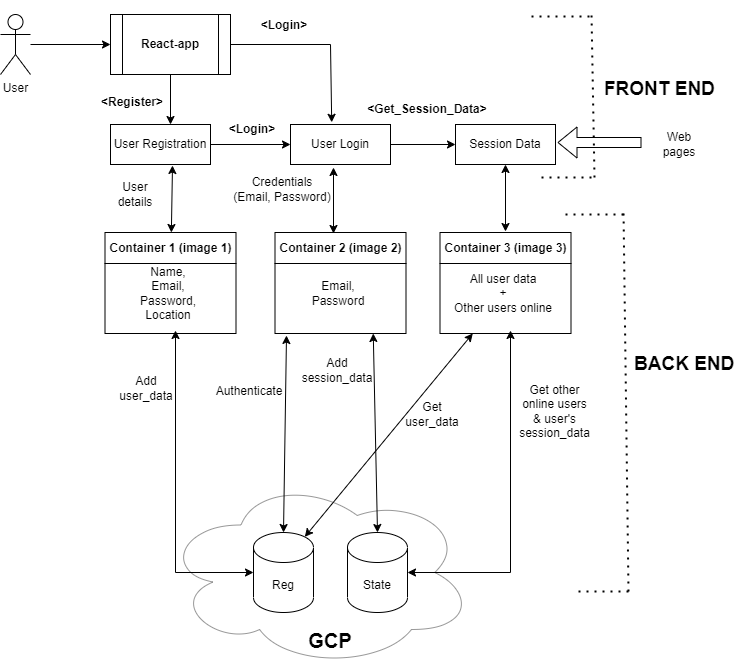
\includegraphics[scale=1, width=12cm,height=12cm]{PROBLEM 2/Flowchart.png}
    \caption{\textbf{\textit{Flowchart describing the operations that I	have performed.}}}
    \label{fig:flowchart}
\end{figure}

\section{Steps}
\subsection{Configure environment}
% \begin{enumerate}
%     \item 
% \end{enumerate}

\begin{enumerate}
    \item Create images for all the given code and front-end (i have created the front-end in React)
    \newline
    \textbf{Note}: Download the service account key from GCP IAM. In the docker file, copy the file to the container, and set it as an Environment variable as follows
    
\definecolor{backcolour}{RGB}{242, 242, 242}

\lstset{
    backgroundcolor=\color{backcolour},
    basicstyle=\small\ttfamily,
    breaklines=true,
    captionpos=b,
    frame=single,
    keywordstyle=\color{blue},
    language=,
    numbers=left,
    numbersep=5pt,
    numberstyle=\tiny\color{gray},
    showspaces=false,
    showstringspaces=false,
    showtabs=false,
    stringstyle=\color{red},
    tabsize=2
}


\begin{lstlisting}[caption={Dockerfile Code snippet}]
COPY assignment-2-390620-60700558380c.json /app/assignment-2-390620-60700558380c.json

ENV GOOGLE_APPLICATION_CREDENTIALS /app/assignment-2-390620-60700558380c.json
\end{lstlisting}
    This will allow the containers to access the collection in Firestore.
    \item Create separate repositories for all containers (3 containers: back-end; 1 container: front-end) in \textbf{Artifact Registry}.
    \item Push the images to the respective repositories
    \item Using the images, create services for all the containers, in \textbf{Cloud run} (with proper \textbf{PORT} and other configuration)
\end{enumerate}
\subsection{Control and data flow of the deployments}
\begin{enumerate}
    \item User performs registration
    \item Send a POST request to Container-1 (API: /A2/register), with all \textit{user\_data}.
    \item Registration by \textbf{Container-1}:
    \begin{enumerate}
        \item Create record in collection \textbf{"Reg"} with \textit{user\_data} (shown below)
        \lstdefinestyle{mystyle}{
    backgroundcolor=\color{backcolour},
    commentstyle=\color{codegreen},
    keywordstyle=\color{magenta},
    numberstyle=\tiny\color{codegray},
    stringstyle=\color{codepurple},
    basicstyle=\ttfamily\footnotesize,
    breakatwhitespace=false,
    breaklines=true,
    captionpos=b,
    keepspaces=true,
    numbers=left,
    numbersep=5pt,
    showspaces=false,
    showstringspaces=false,
    showtabs=false,
    tabsize=2
}

\lstset{style=mystyle}

\begin{lstlisting}[language=Python]
{
    'Name': <name>,
    'Password': <password>,
    'Email': <email>,
    'Location': <location>
}

\end{lstlisting}
        \item Return response (success/failure).
    \end{enumerate}
    \item Front-end: re-direct to \textbf{login page} after successful registration (API: /A2/login).
    \item User enters credentials.
    \item Authentication by \textbf{Container-2}
    \begin{enumerate}
        \item Fetch the respective document from the collection "Reg"  
        \item Validate credentials
        \item Return Success/Failure
    \end{enumerate}
    \item After successful authentication, 
    \begin{enumerate}
        \item If the user is logging in for the 1st time, create a \textit{session\_data} document(shown below) in the collection "state", with the user\_email as the document id.
        \lstdefinestyle{mystyle}{
    backgroundcolor=\color{backcolour},
    commentstyle=\color{codegreen},
    keywordstyle=\color{magenta},
    numberstyle=\tiny\color{codegray},
    stringstyle=\color{codepurple},
    basicstyle=\ttfamily\footnotesize,
    breakatwhitespace=false,
    breaklines=true,
    captionpos=b,
    keepspaces=true,
    numbers=left,
    numbersep=5pt,
    showspaces=false,
    showstringspaces=false,
    showtabs=false,
    tabsize=2
}

\lstset{style=mystyle}

\begin{lstlisting}[language=Python]
{
    'Online': True,
    'Offline': False,
    'Timestamp': <current_system_time>
}
\end{lstlisting}
    \item Else, just update the fields (toggle Online \& Offline, update the current timestamp of system) 
    \end{enumerate}
    \item Redirect to \textbf{session\_data page} (API: /A2/sessionData/\textless email\textgreater)
    \item Session data from \textbf{Container-3}
    \begin{enumerate}
        \item Fetch \textit{user\_data} from the collection "Reg", \textit{session\_data} from the collection "state", by matching with the \textless email\textgreater
        \item Display all the user details
        % \item Fetch all user emails from the collection "Reg"
        \item To display the other users, who are online, filter out all documents in the collection "state" where the key \textbf{"Online" is True}. (API: /A2/sessionData/usersOnline/\textless email \textgreater)
        \item Display the filtered document ids (except the current user who has logged in).
    \end{enumerate}
    \item Logout by Container-3:
    \begin{enumerate}
        \item On clicking logout, \textbf{end the current session}. (API: /A2/sessionData/\textless email \textgreater/logout)
        \item Update the \textit{session\_data} in the collection "state" (toggle Online \& Offline fields)
        \item Re-direct to the Login page.
    \end{enumerate}


\end{enumerate}

\newpage
\chapter{Screenshots}
\section{Environment setup}
% \newpage
% \subsection{Images build and push}
% \newpage
% \begin{figure}[htp]
%     \centering
%     \fbox{\includegraphics[scale=1, width=15cm,height=7.5cm]{PROBLEM 2/Screenshots/1. Setup/}}
%     \caption{\textbf{\textit{  }}}
%     \label{fig:}
% \end{figure}

\begin{figure}[htp]
    \centering
    \fbox{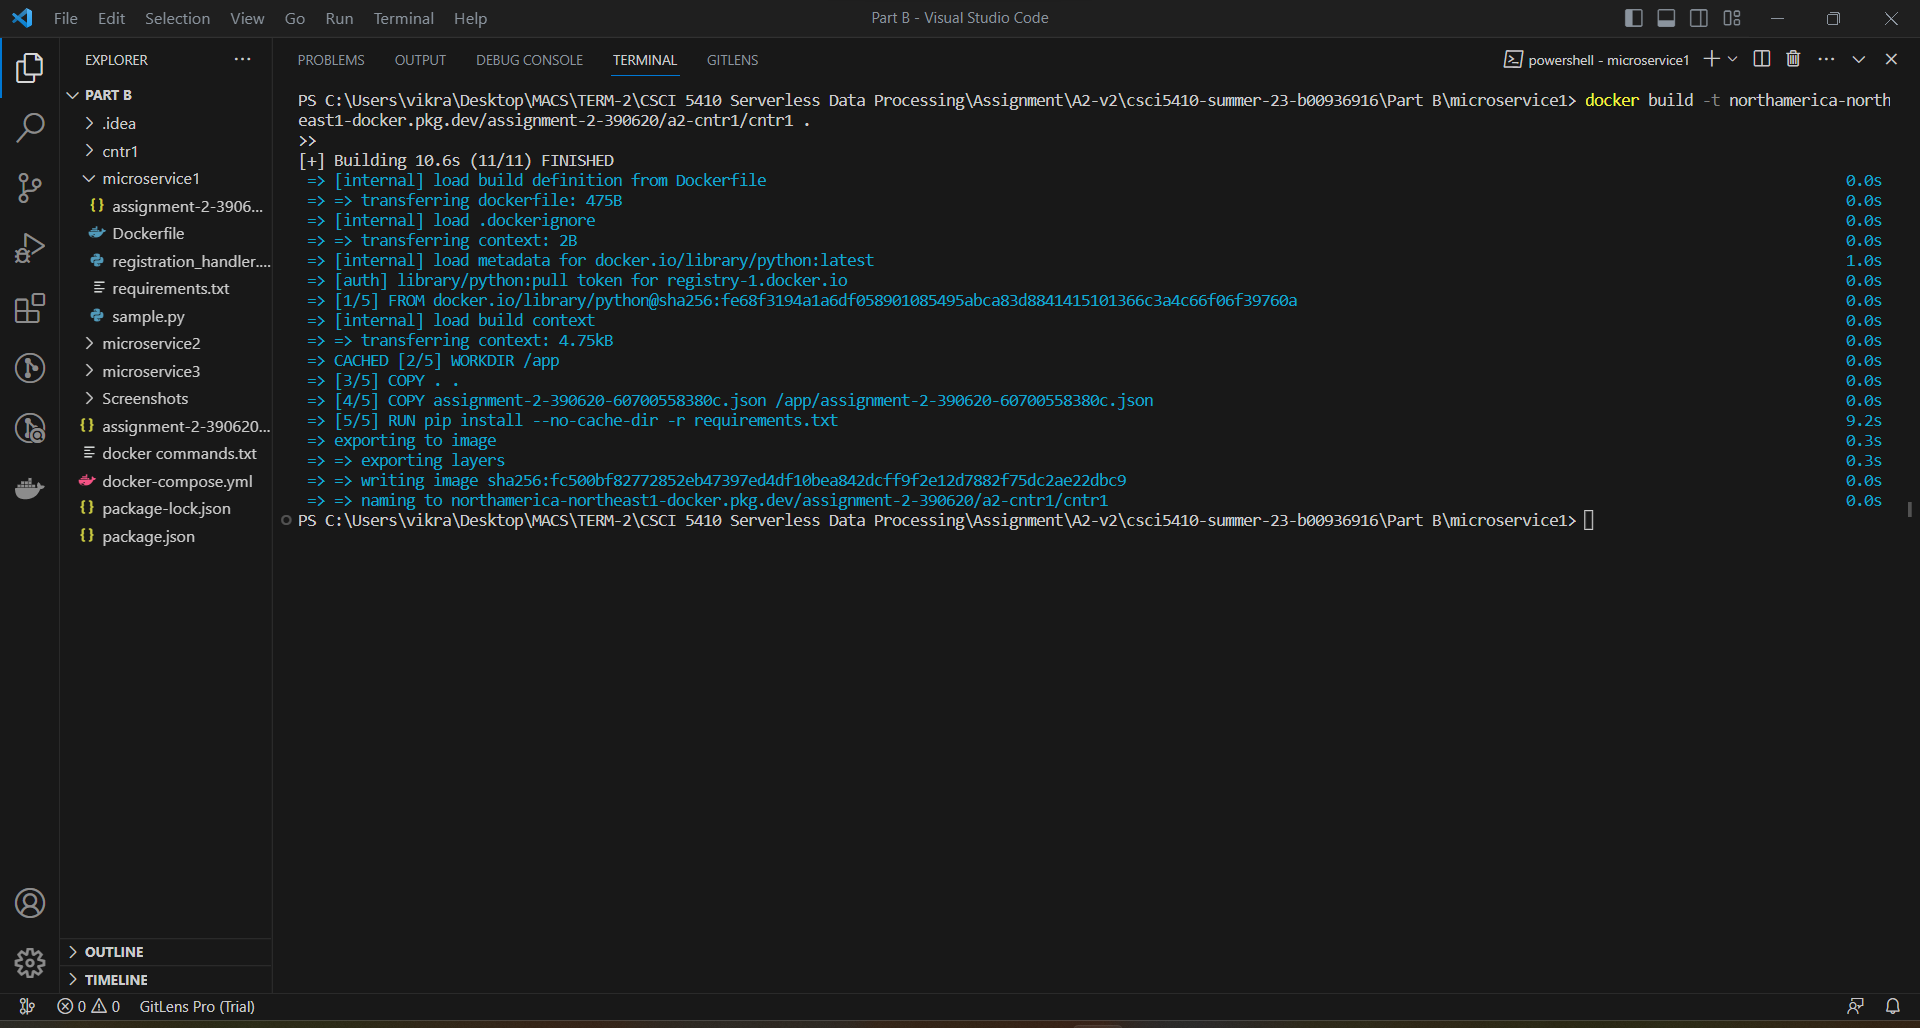
\includegraphics[scale=1, width=15cm,height=7.5cm]{PROBLEM 2/Screenshots/1. Setup/1. Image build/1.1 build cntr1.png}}
    \caption{\textbf{\textit{ Build container 1 }}}
    \label{fig:}
\end{figure}
\begin{figure}[htp]
    \centering
    \fbox{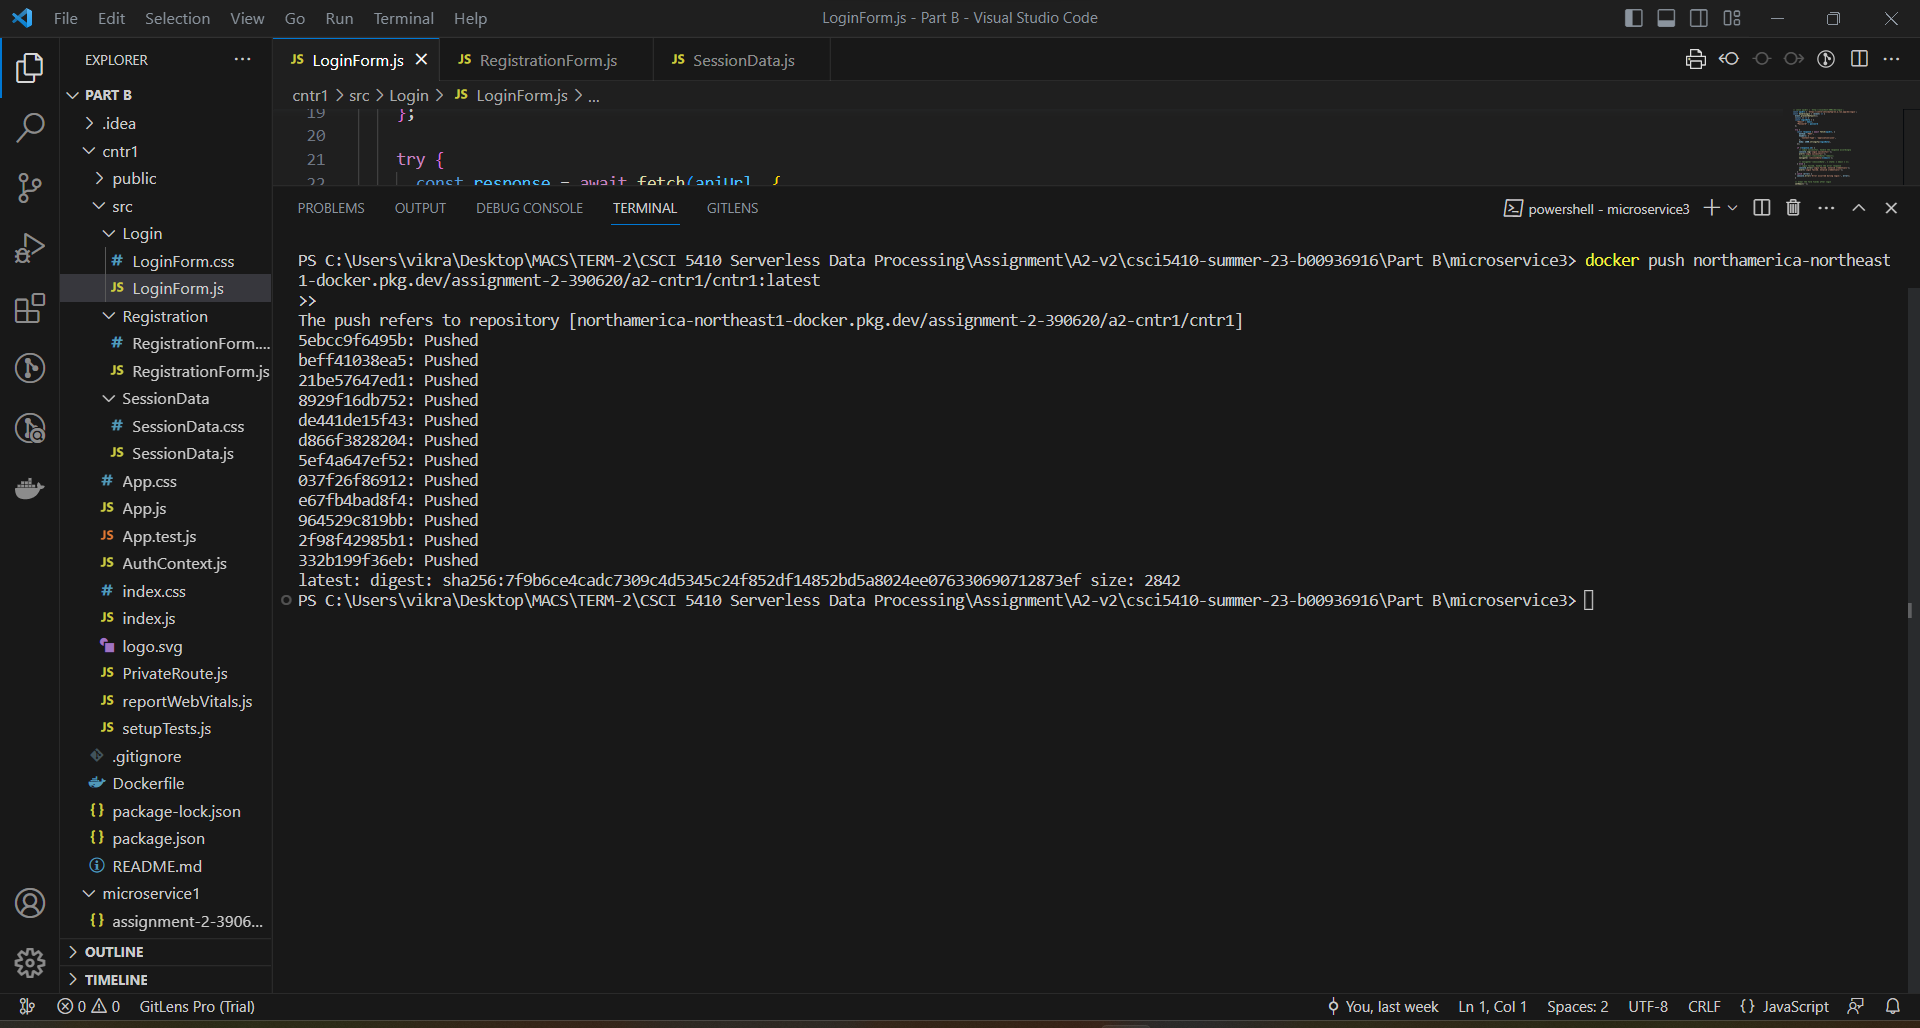
\includegraphics[scale=1, width=15cm,height=7.5cm]{PROBLEM 2/Screenshots/1. Setup/1. Image build/1.2 push cntr1.png}}
    \caption{\textbf{\textit{ Push container 1 }}}
    \label{fig:push-container-1}
\end{figure}


\begin{figure}[htp]
    \centering
    \fbox{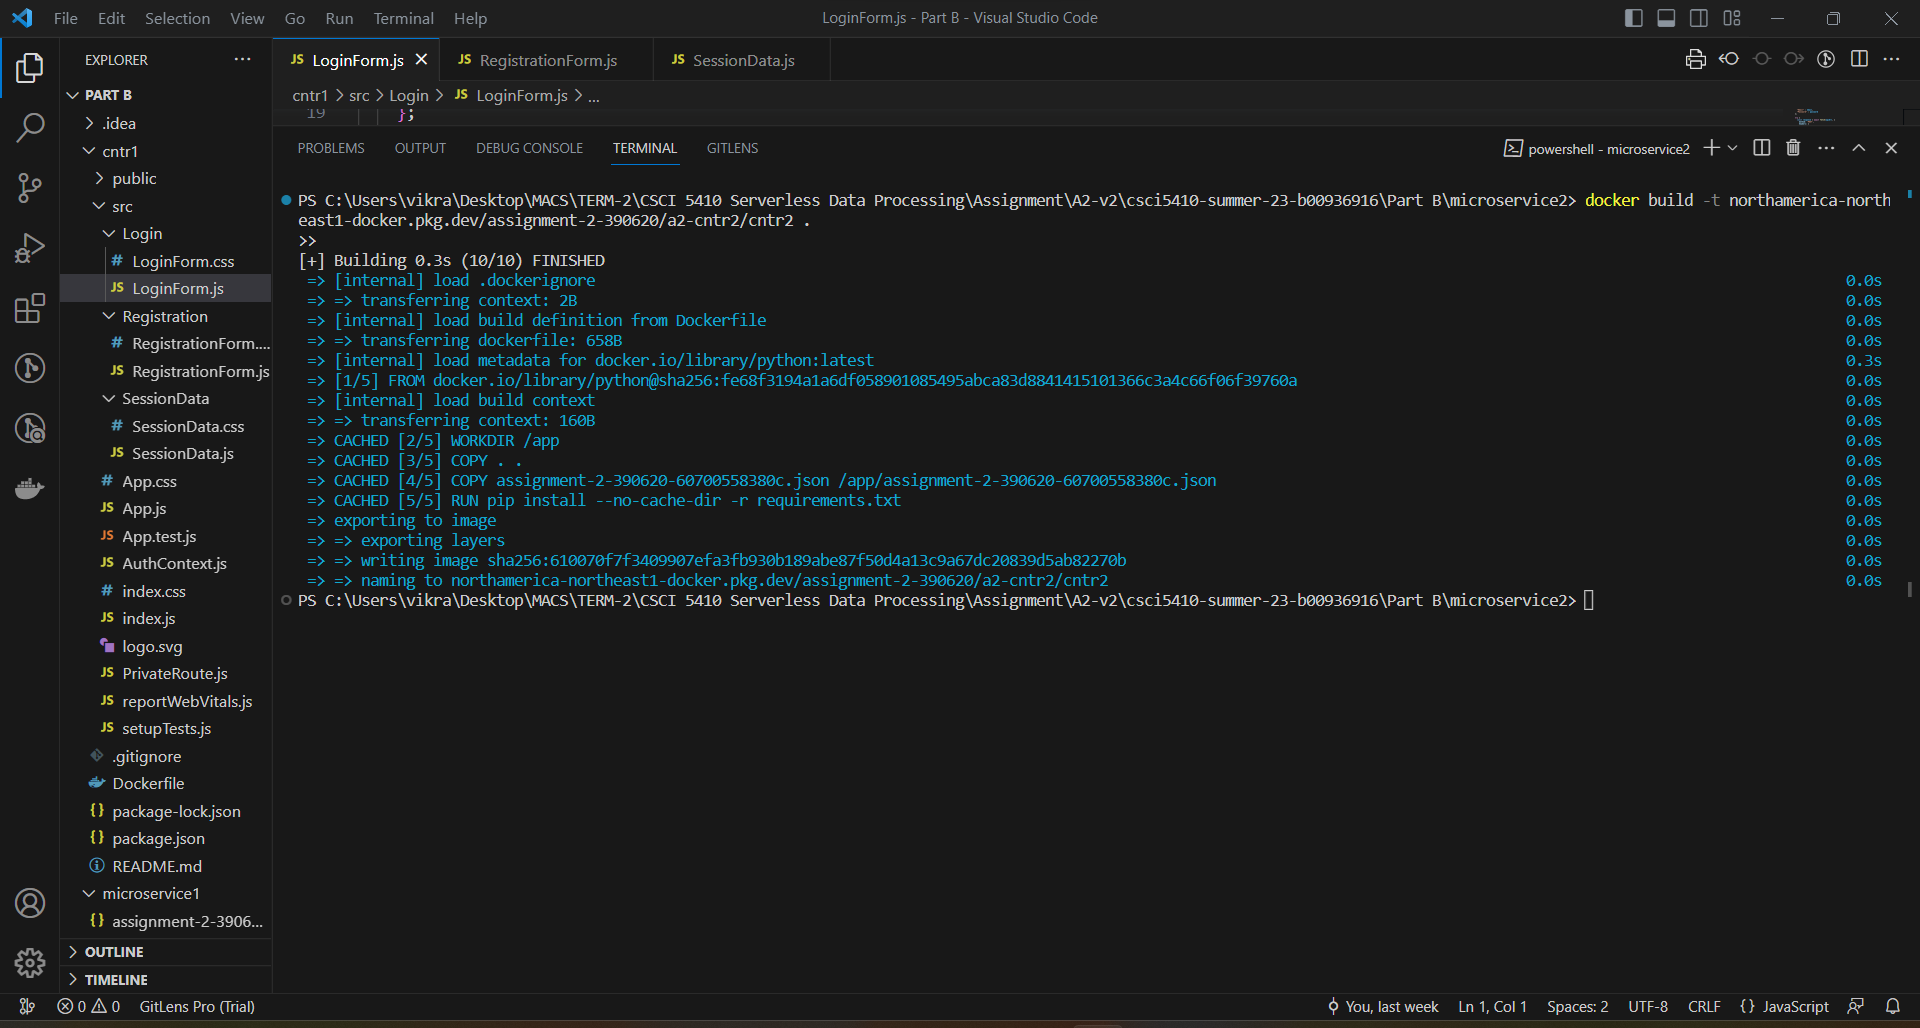
\includegraphics[scale=1, width=15cm,height=7.5cm]{PROBLEM 2/Screenshots/1. Setup/1. Image build/2.1 build cntr2.png}}
    \caption{\textbf{\textit{ Build container 2 }}}
    \label{fig:}
\end{figure}
\begin{figure}[htp]
    \centering
    \fbox{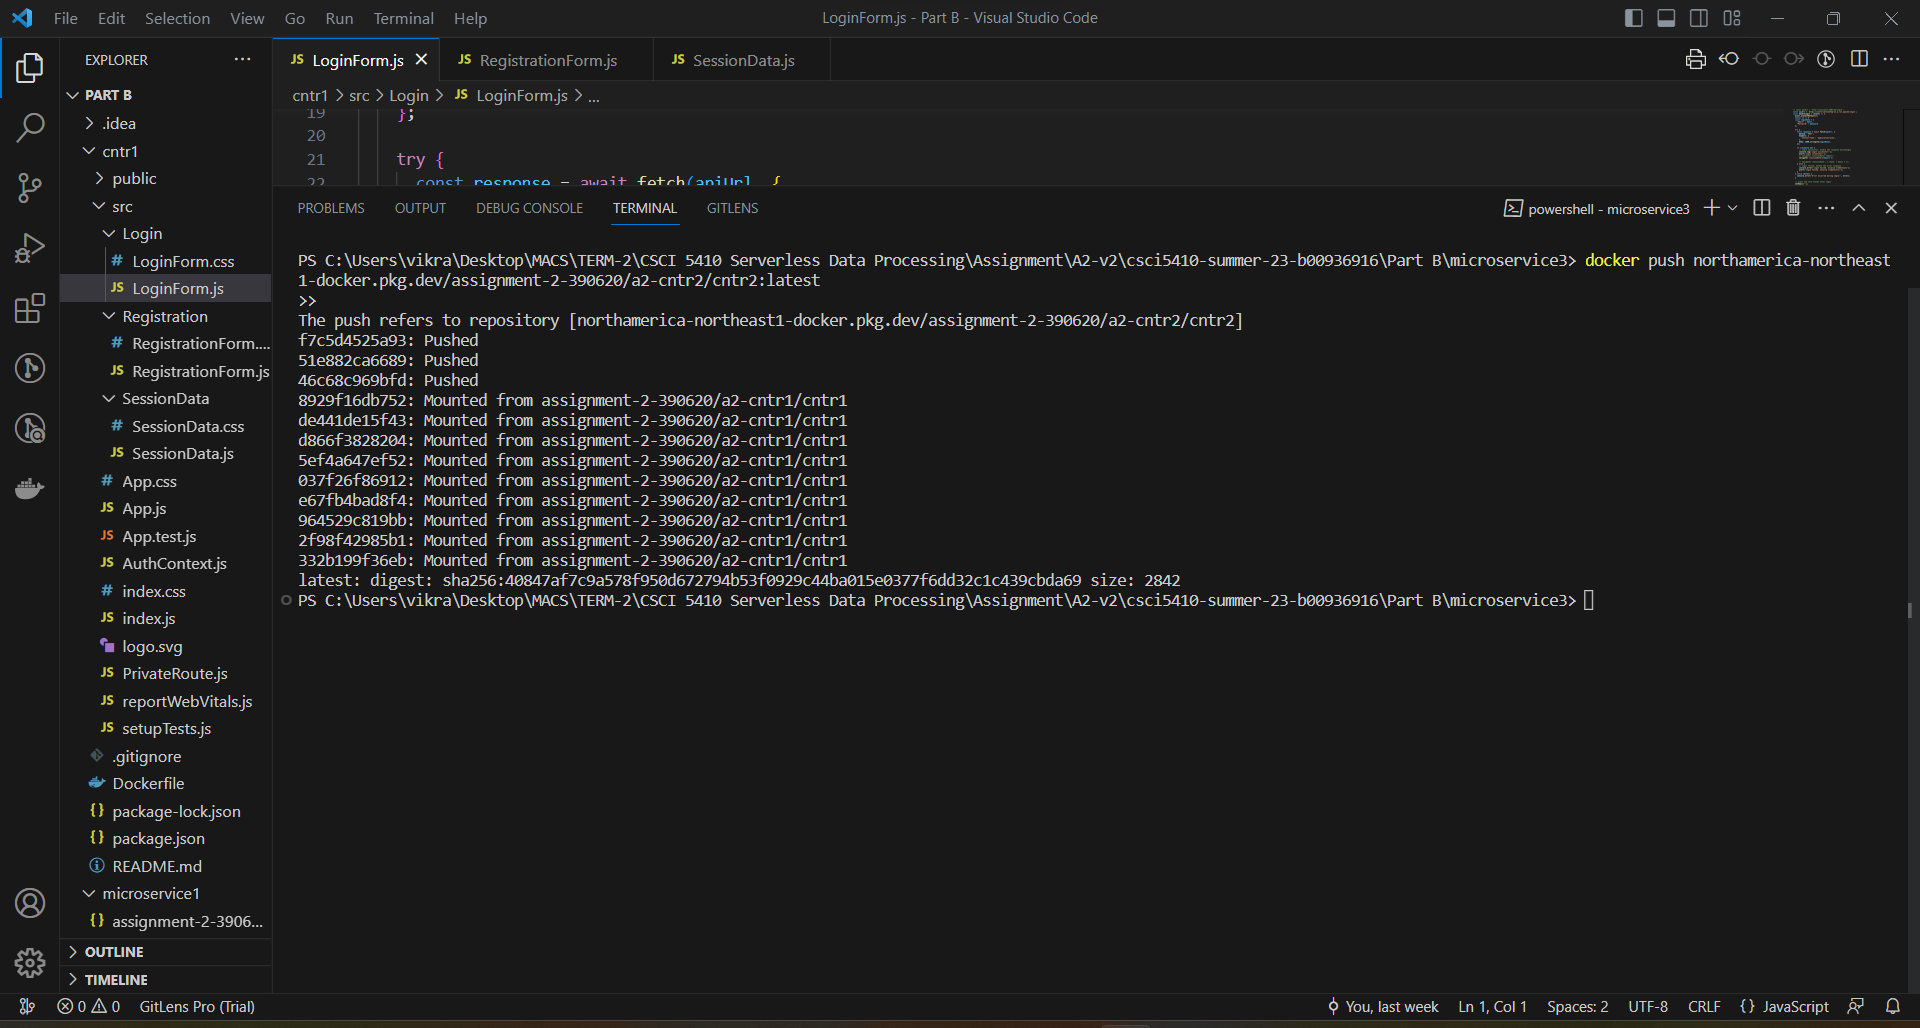
\includegraphics[scale=1, width=15cm,height=7.5cm]{PROBLEM 2/Screenshots/1. Setup/1. Image build/2.2 push cntr2.png}}
    \caption{\textbf{\textit{ Push container 2 }}}
    \label{fig:push-container-2}
\end{figure}


\begin{figure}[htp]
    \centering
    \fbox{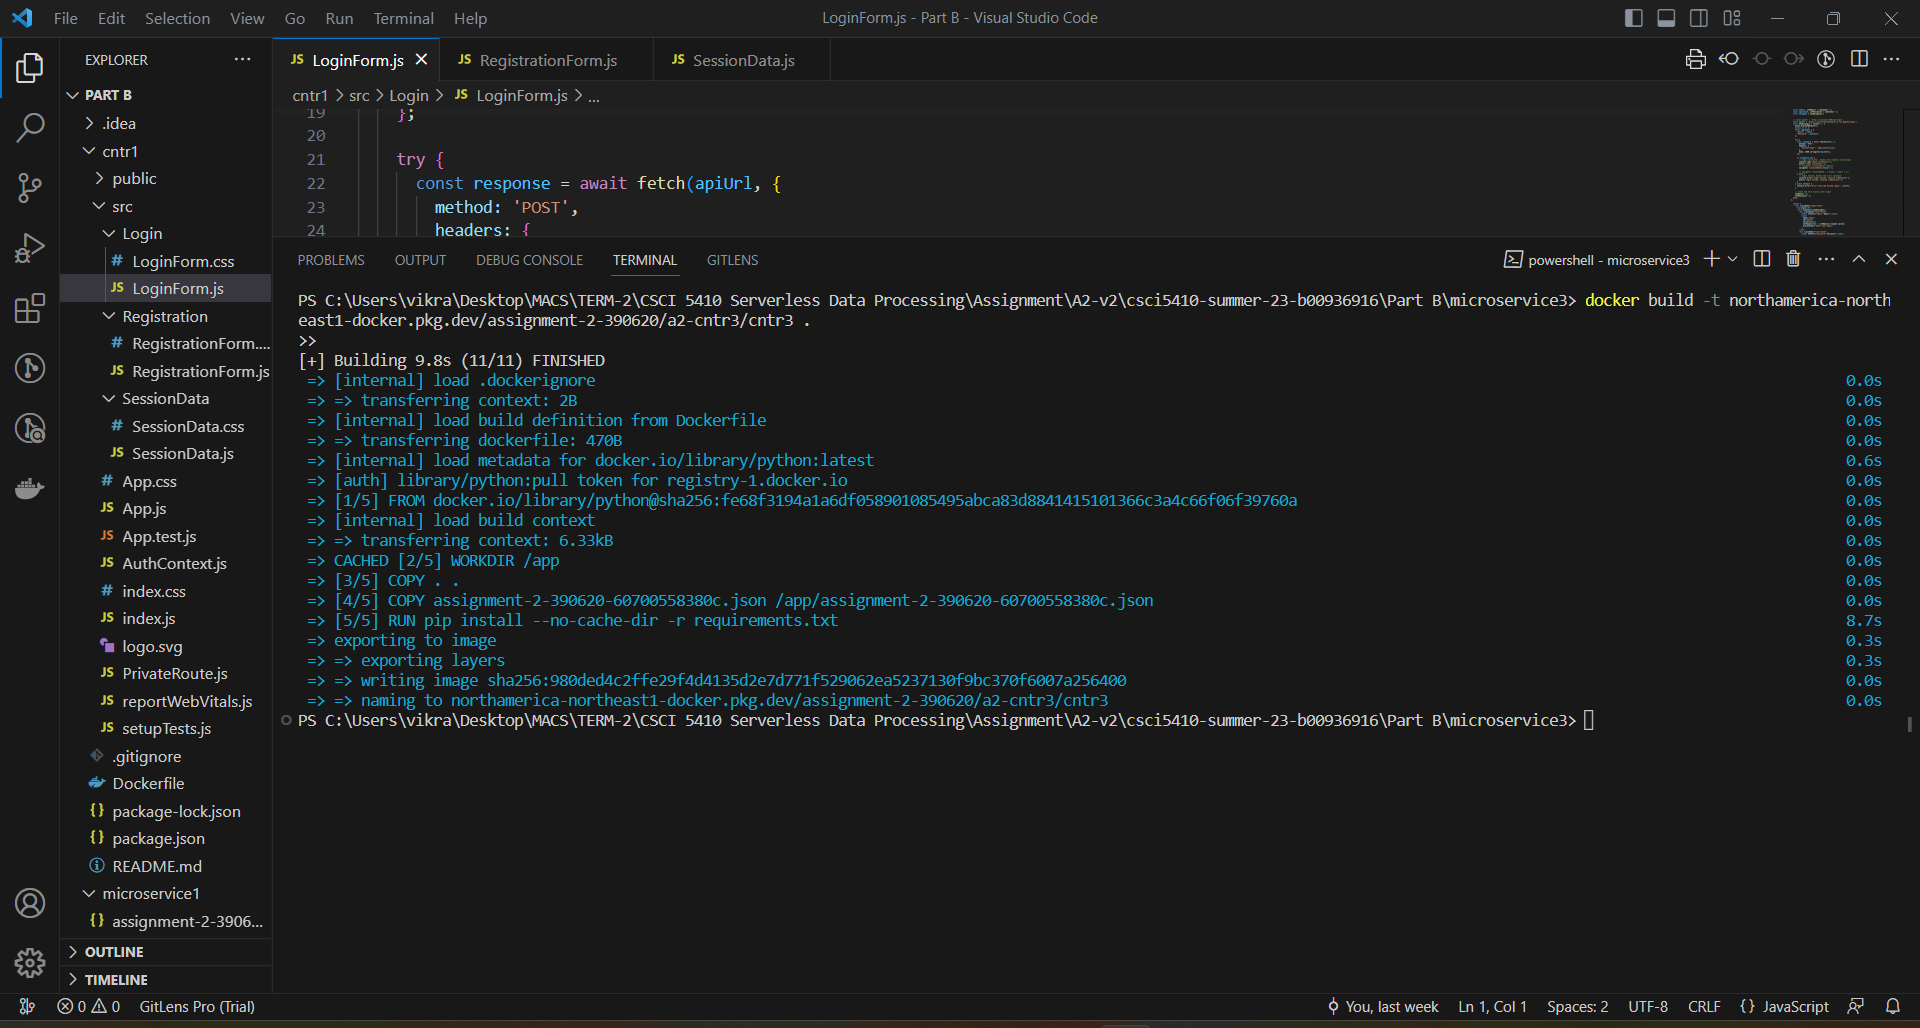
\includegraphics[scale=1, width=15cm,height=7.5cm]{PROBLEM 2/Screenshots/1. Setup/1. Image build/3.1 build cntr3.png}}
    \caption{\textbf{\textit{ Build container 3 }}}
    \label{fig:}
\end{figure}
\begin{figure}[htp]
    \centering
    \fbox{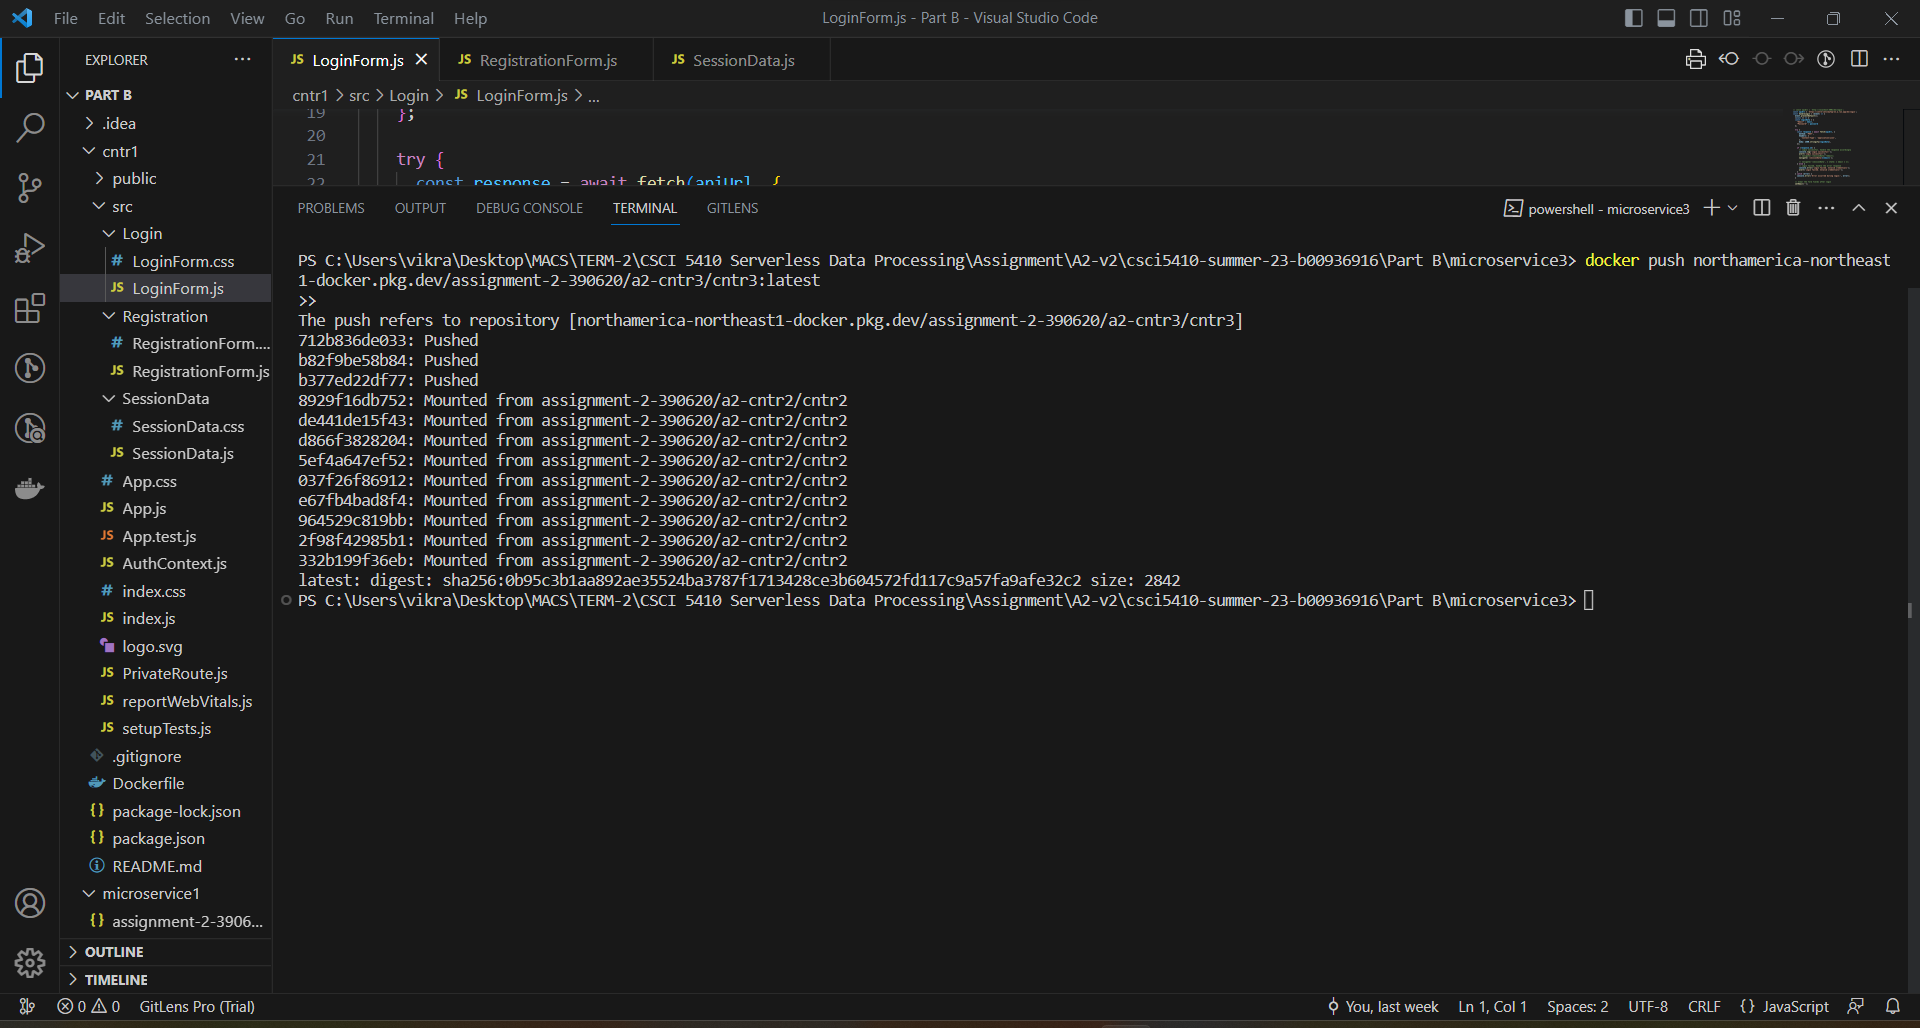
\includegraphics[scale=1, width=15cm,height=7.5cm]{PROBLEM 2/Screenshots/1. Setup/1. Image build/3.2 push cntr3.png}}
    \caption{\textbf{\textit{ Push container 3 }}}
    \label{fig:push-container-3}
\end{figure}
\begin{figure}[htp]
    \centering
    \fbox{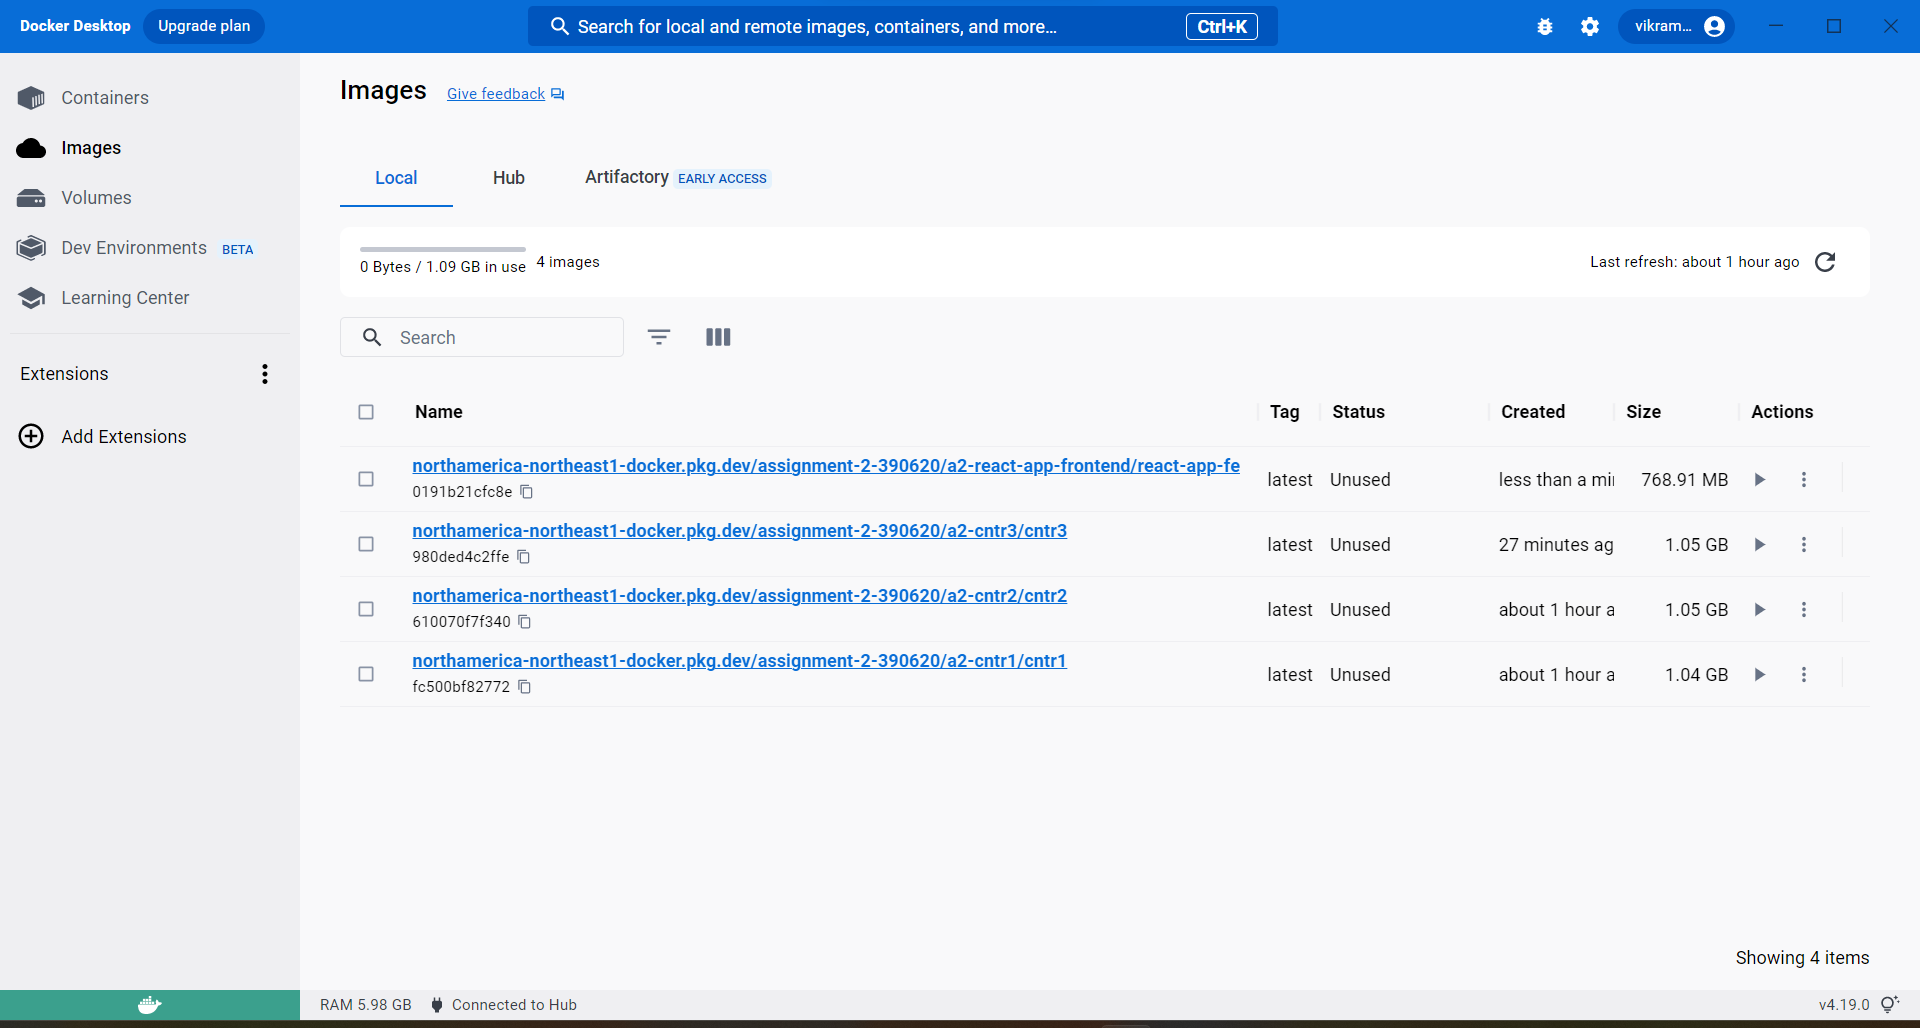
\includegraphics[scale=1, width=15cm,height=7.5cm]{PROBLEM 2/Screenshots/1. Setup/1. Image build/0. images in docker.png}}
    \caption{\textbf{\textit{ Built images listed in Docker Desktop }}}
    \label{fig:}
\end{figure}

\newpage
\subsection{Collections \& Repositories}
% \newpage
\begin{figure}[htp]
    \centering
    \fbox{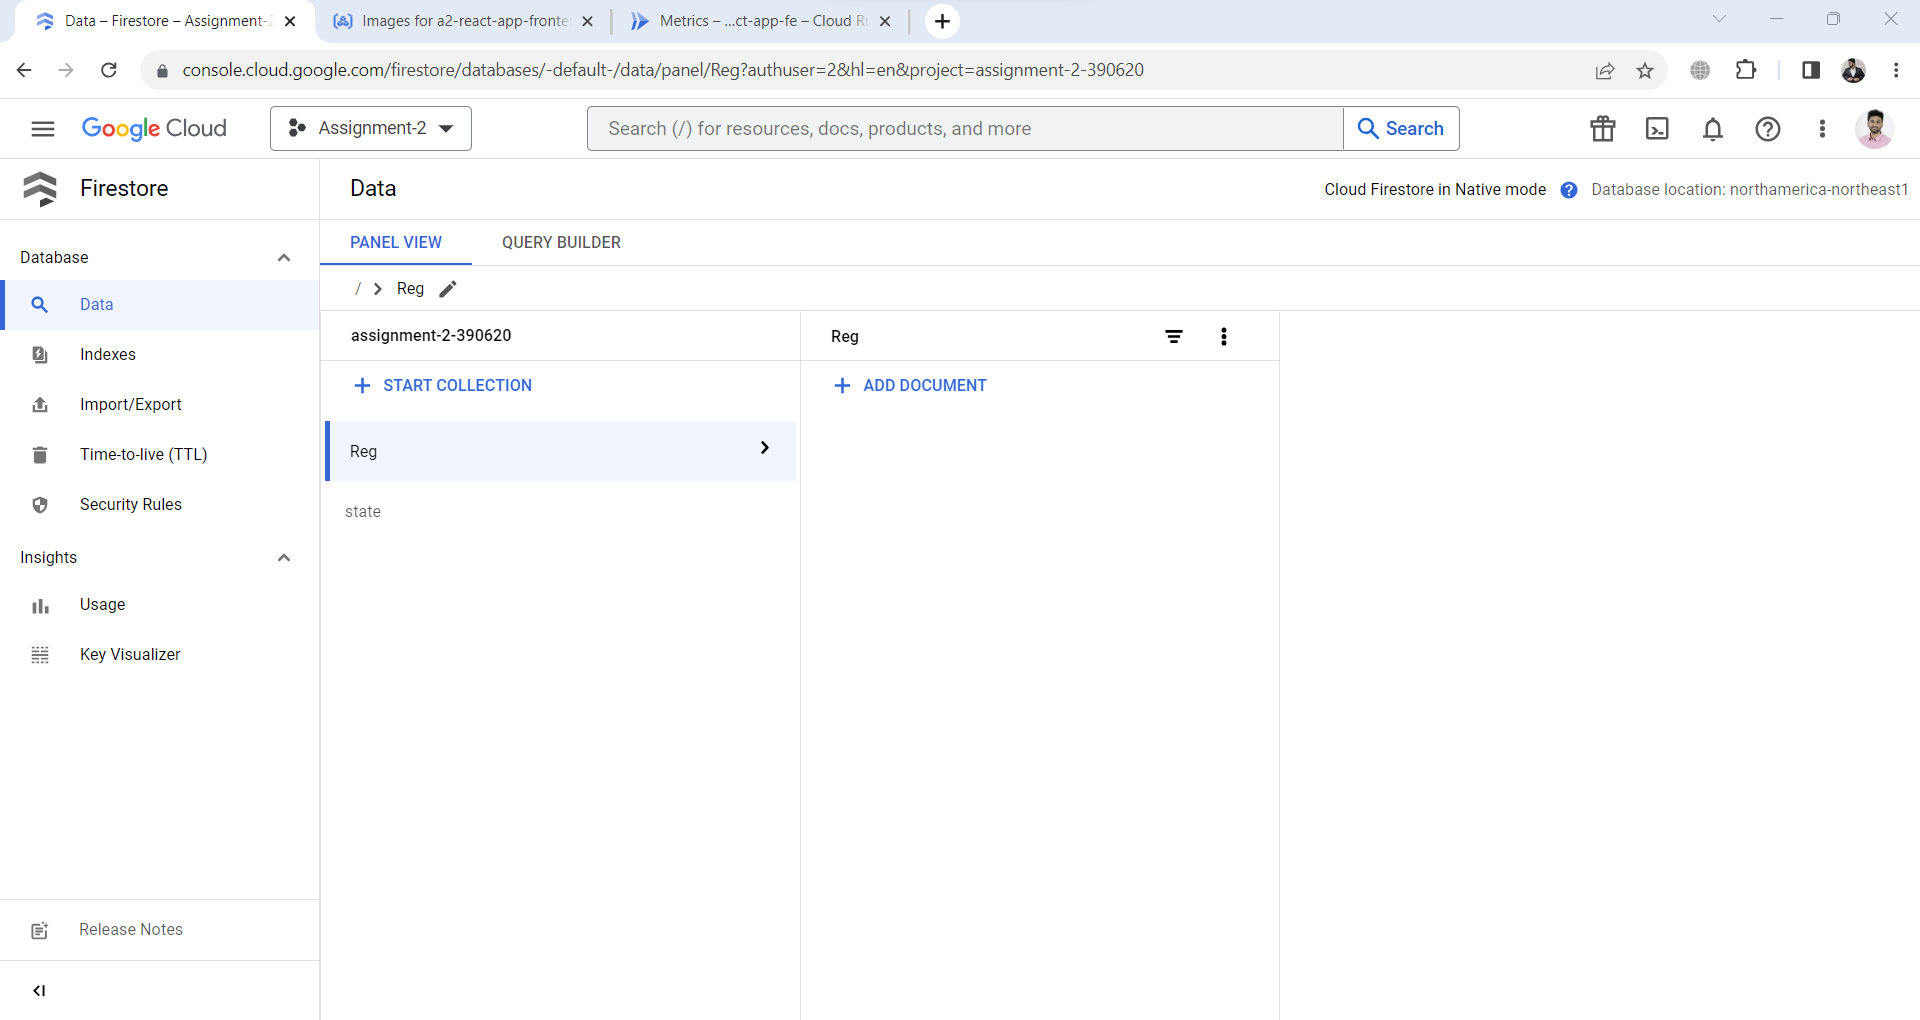
\includegraphics[scale=1, width=15cm,height=7.5cm]{PROBLEM 2/Screenshots/1. Setup/1. Empty Reg.png}}
    \caption{\textbf{\textit{ Empty collection "Reg" }}}
    \label{fig:empty-reg}
\end{figure}

\begin{figure}[htp]
    \centering
    \fbox{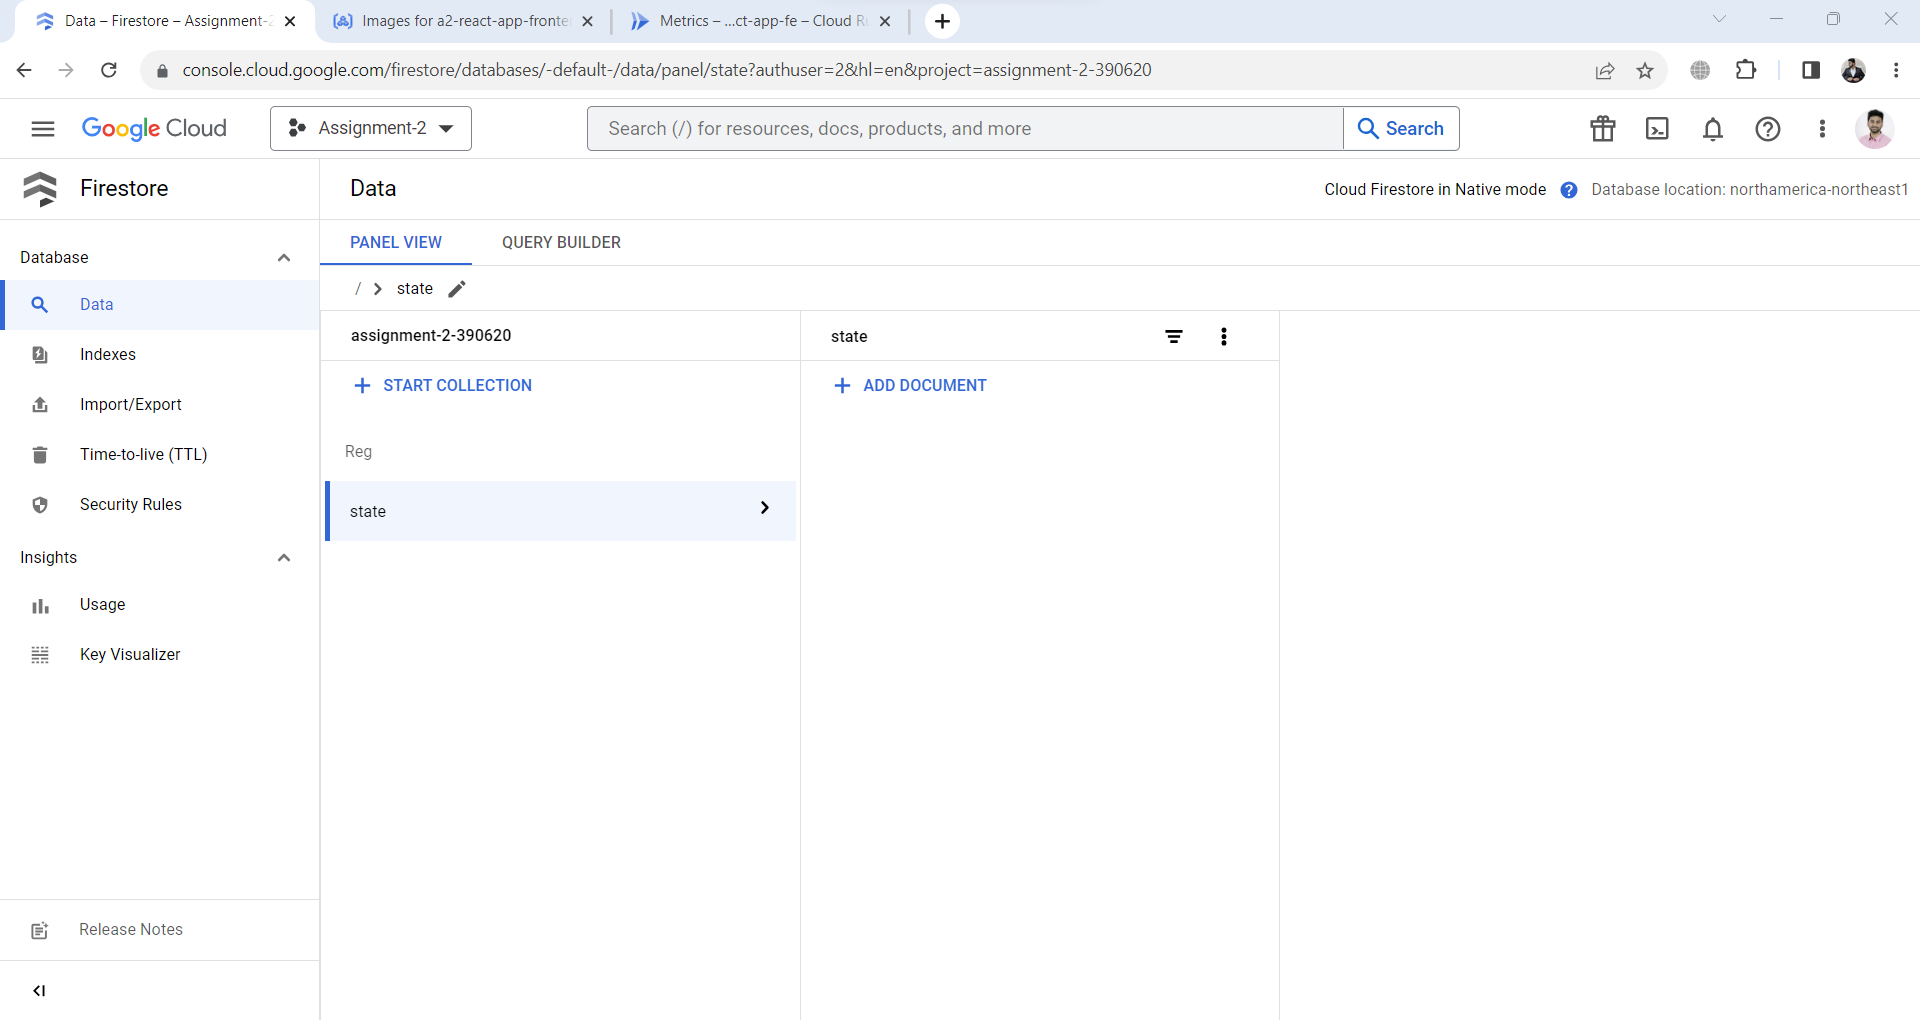
\includegraphics[scale=1, width=15cm,height=7.5cm]{PROBLEM 2/Screenshots/1. Setup/2. Empty state.png}}
    \caption{\textbf{\textit{ Empty collection "state" }}}
    \label{fig:empty-state}
\end{figure}

\begin{figure}[htp]
    \centering
    \fbox{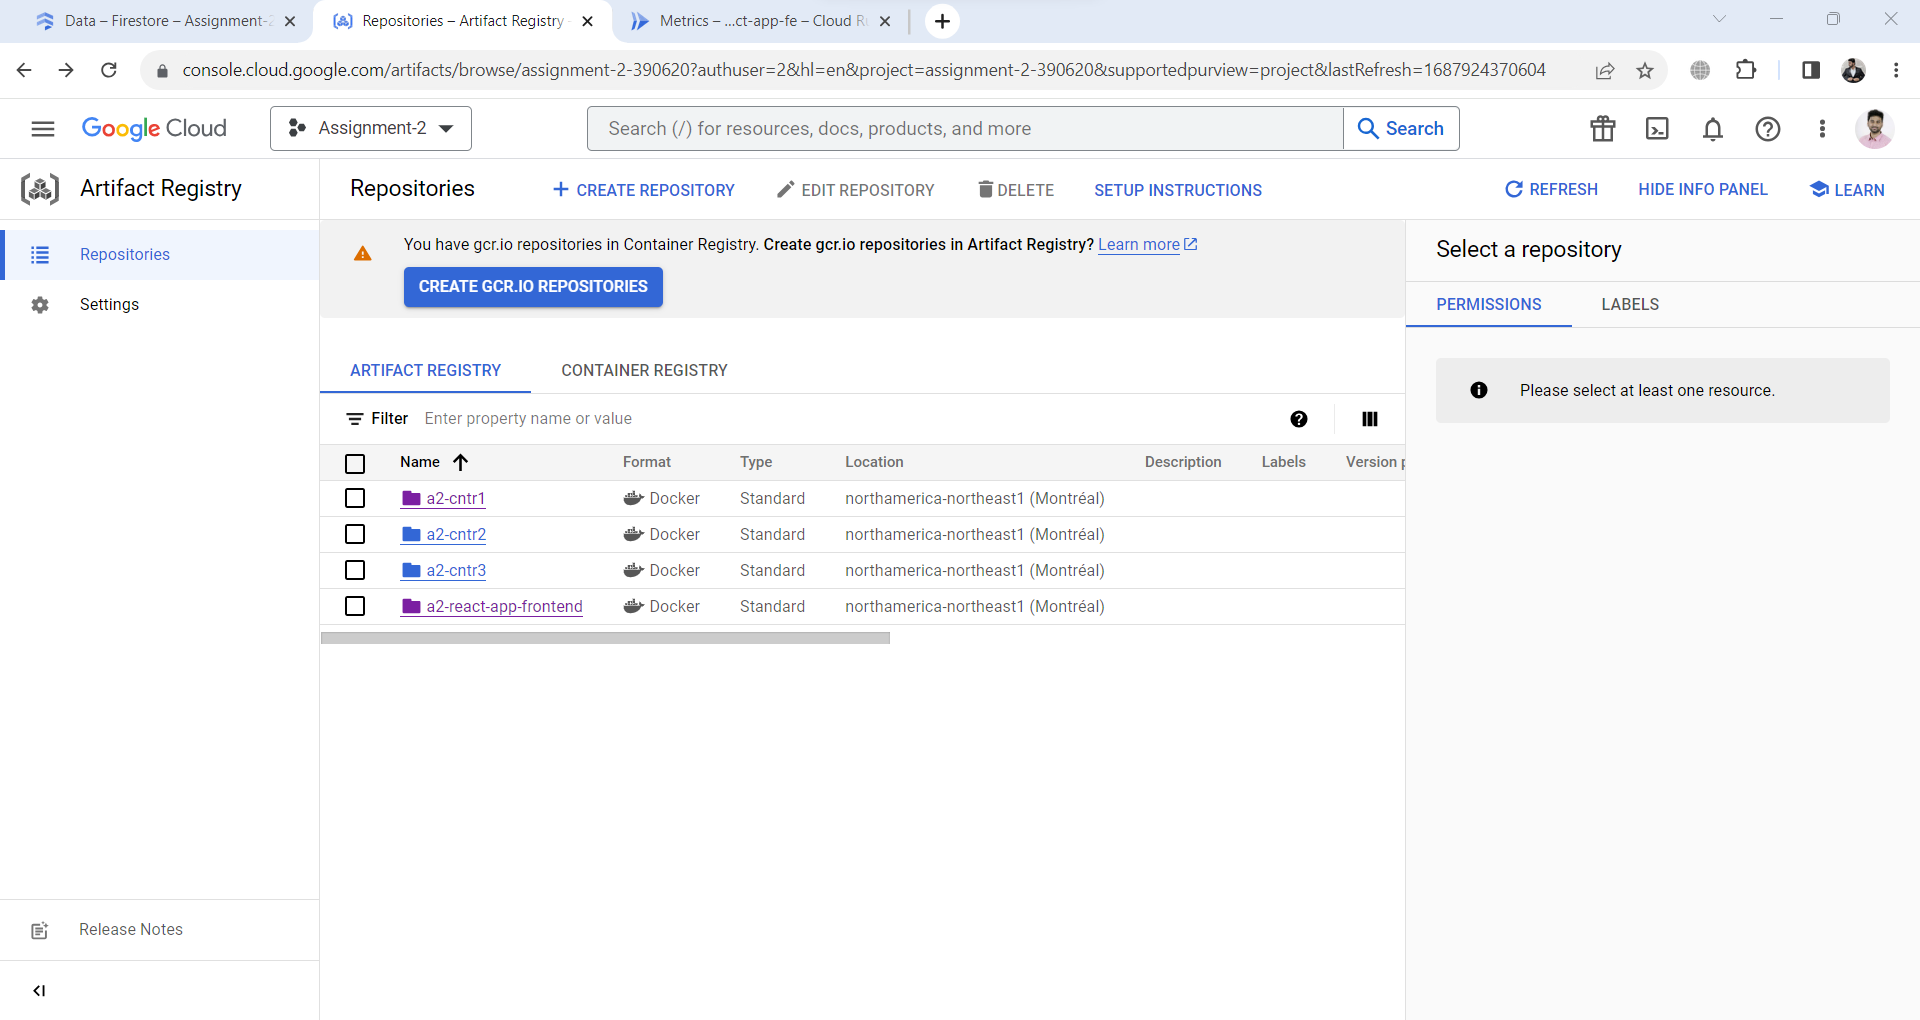
\includegraphics[scale=1, width=15cm,height=7.5cm]{PROBLEM 2/Screenshots/1. Setup/3. Artifact registry repos.png}}
    \caption{\textbf{\textit{ Artifact registry repositories }}}
    \label{fig:Artifact-registry-repo}
\end{figure}

\begin{figure}[htp]
    \centering
    \fbox{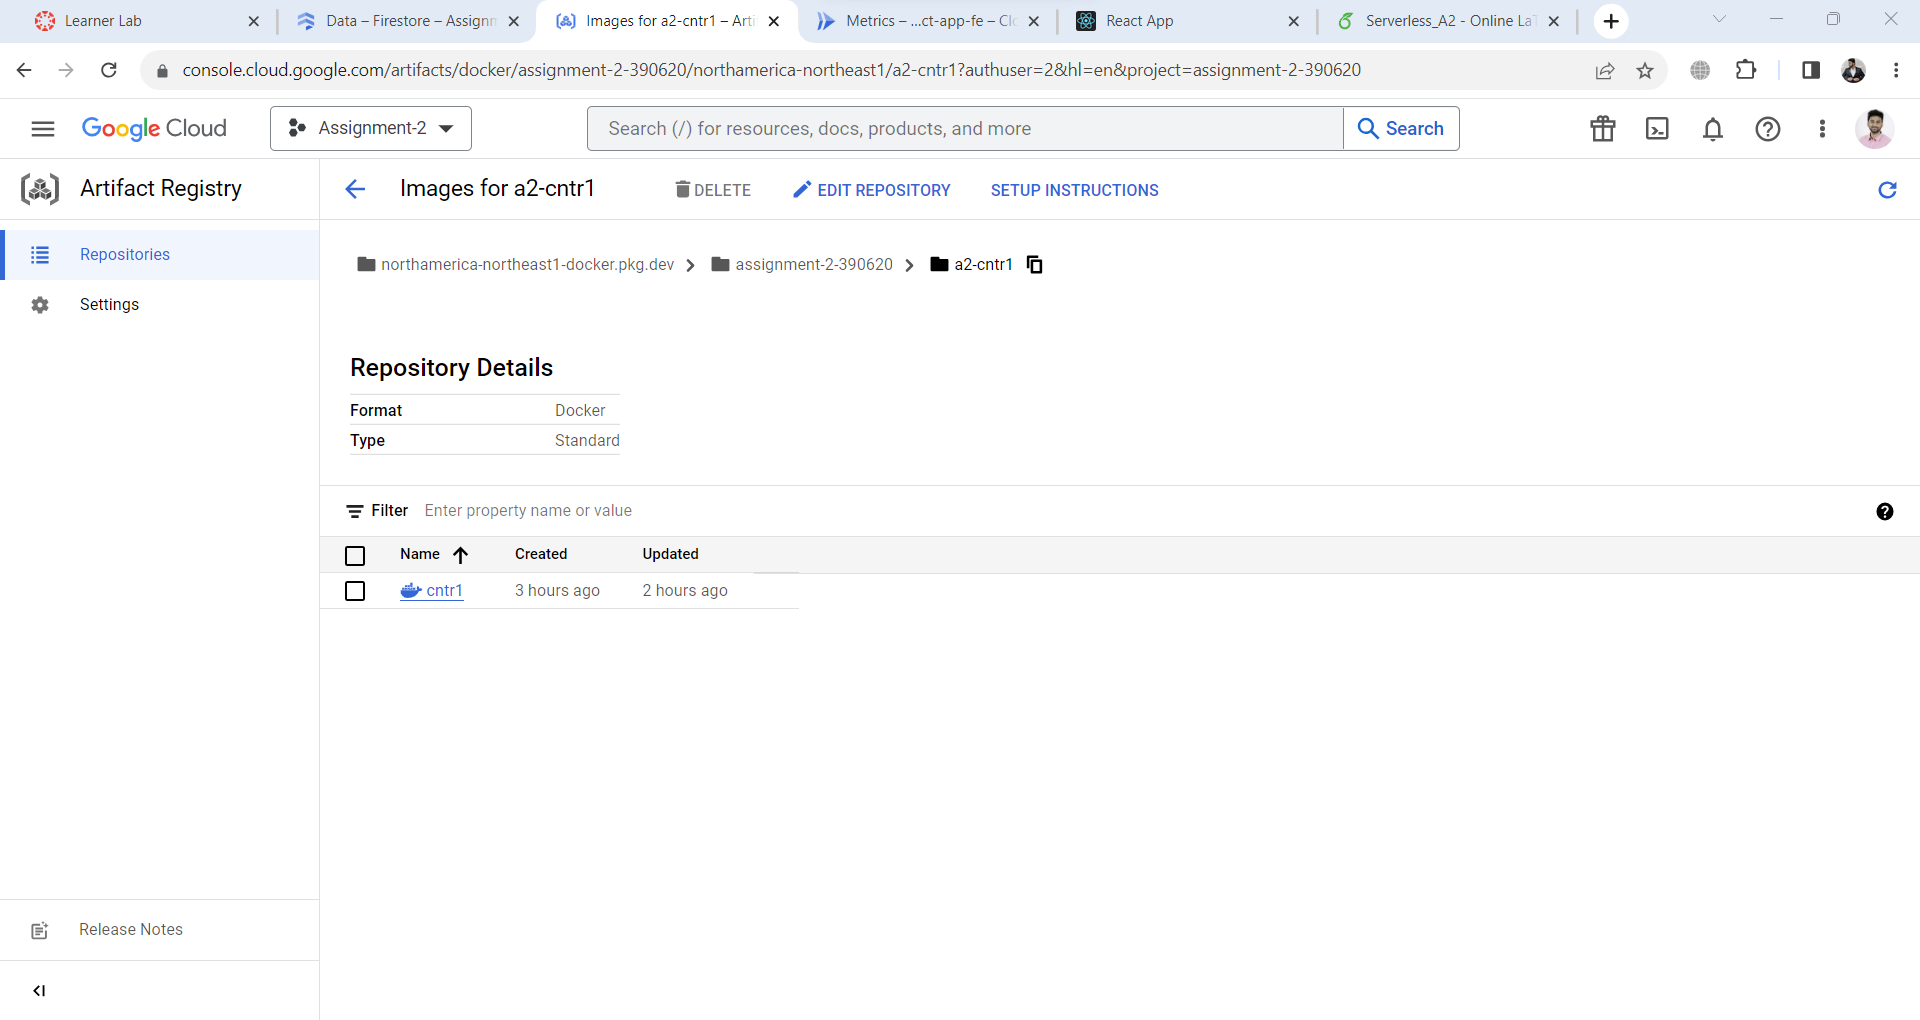
\includegraphics[scale=1, width=15cm,height=7.5cm]{PROBLEM 2/Screenshots/1. Setup/2. artifact reg repos/1. cntr1 image.png}}
    \caption{\textbf{\textit{ Artifact registry repository - container 1 }}}
    \label{fig:Artifact-registry-repo-cntr1}
\end{figure}

\begin{figure}[htp]
    \centering
    \fbox{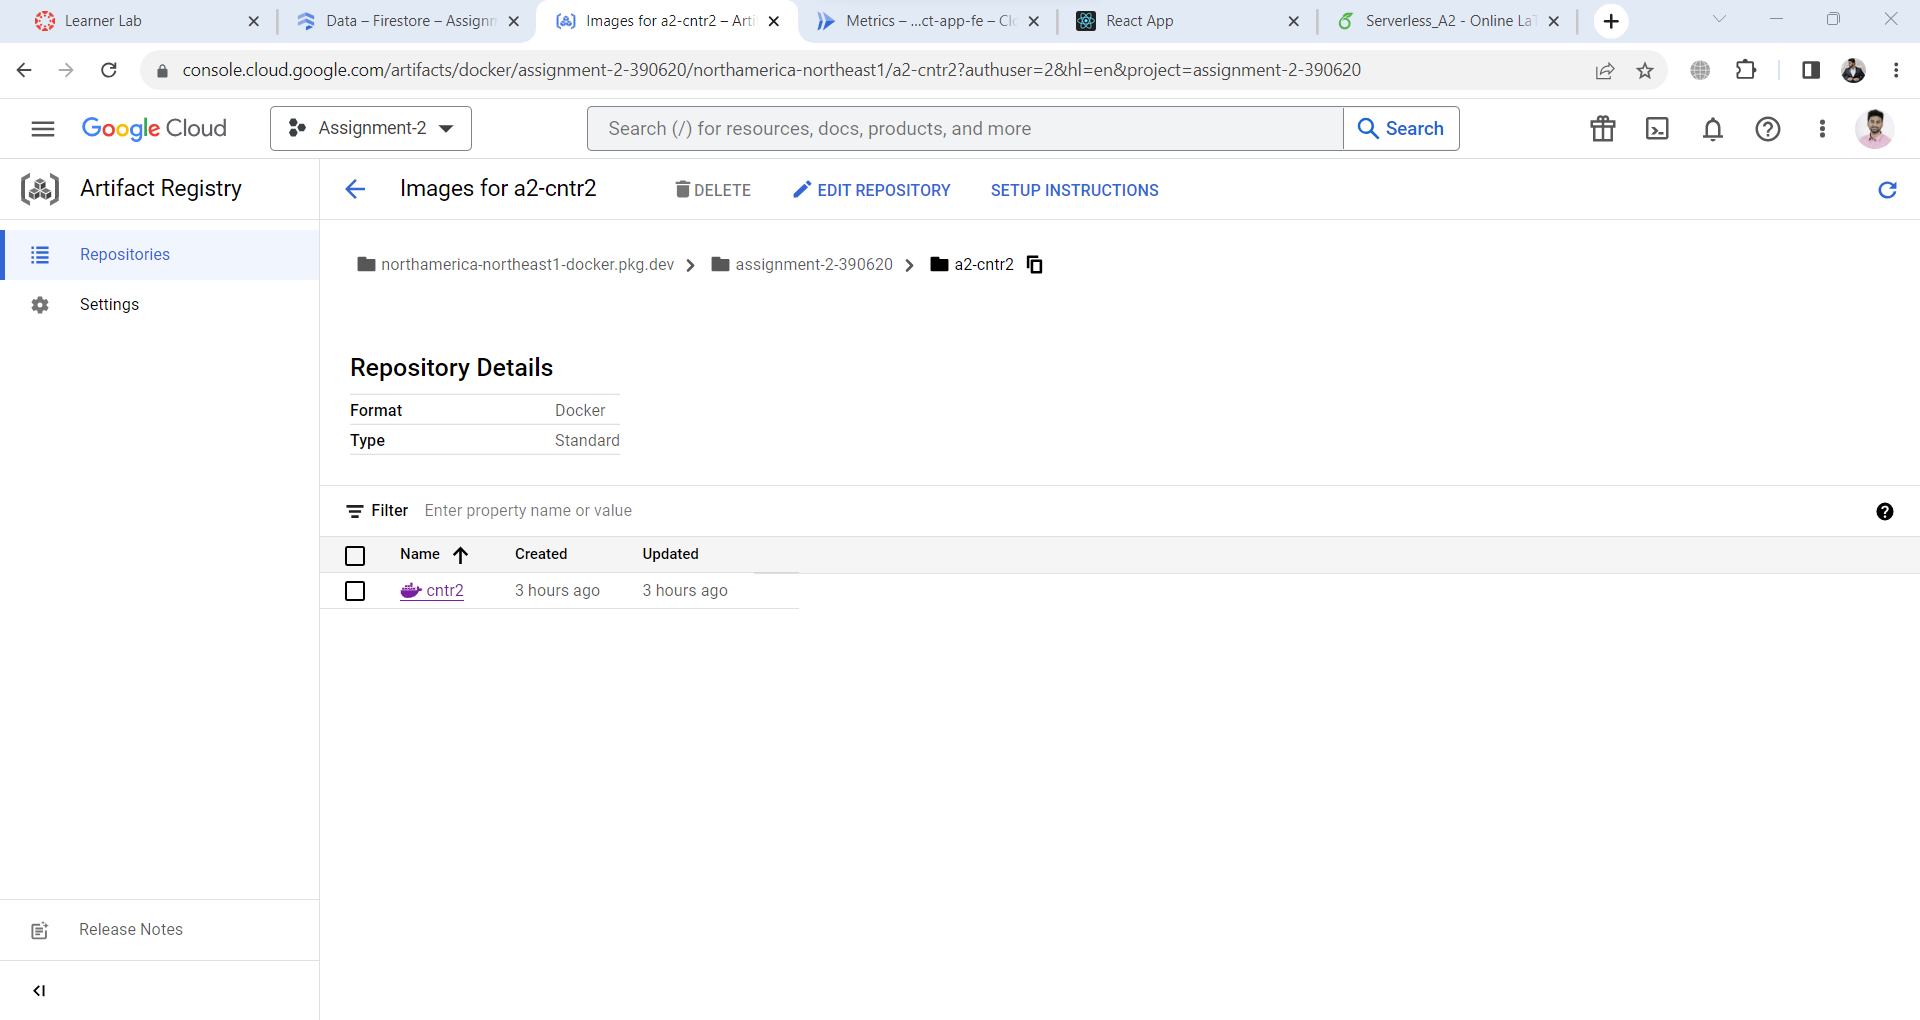
\includegraphics[scale=1, width=15cm,height=7.5cm]{PROBLEM 2/Screenshots/1. Setup/2. artifact reg repos/2. cntr2 image.png}}
    \caption{\textbf{\textit{ Artifact registry repository - container 2 }}}
    \label{fig:Artifact-registry-repo-cntr2}
\end{figure}

\begin{figure}[htp]
    \centering
    \fbox{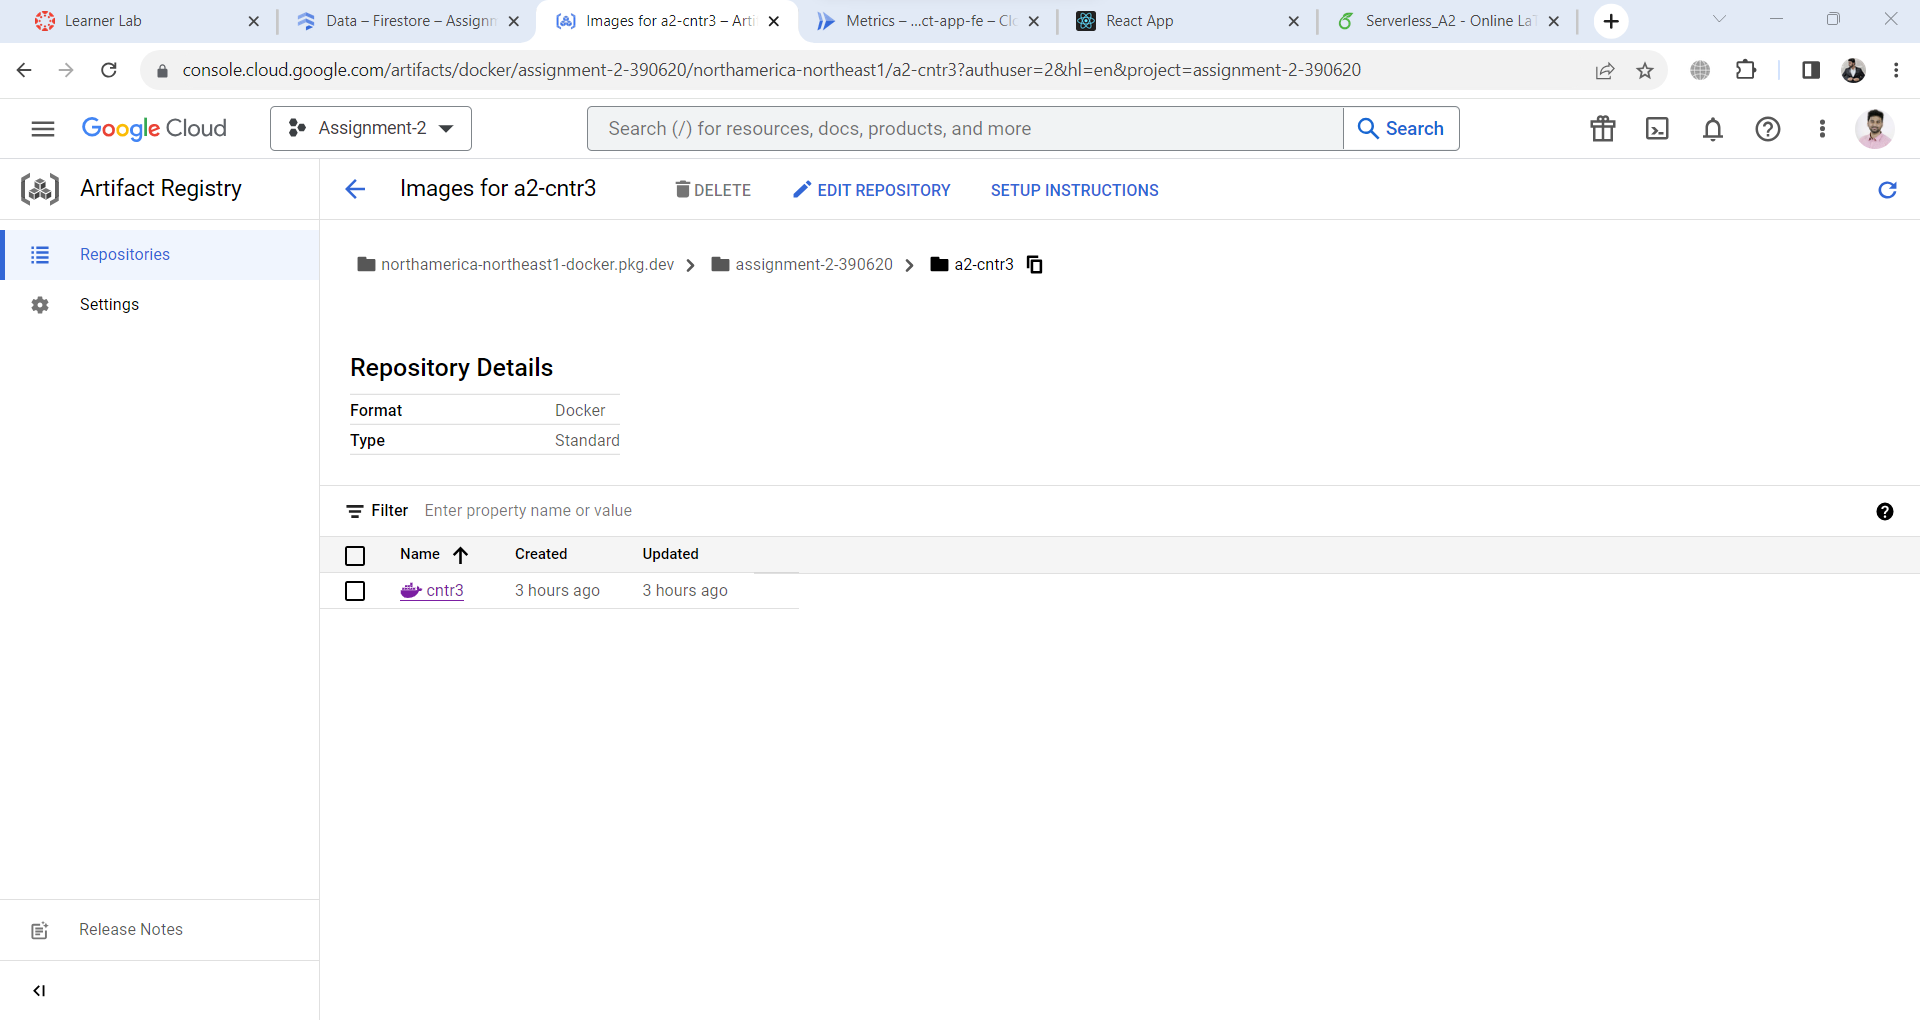
\includegraphics[scale=1, width=15cm,height=7.5cm]{PROBLEM 2/Screenshots/1. Setup/2. artifact reg repos/3. cntr3 image.png}}
    \caption{\textbf{\textit{ Artifact registry repository - container 3 }}}
    \label{fig:Artifact-registry-repo-cntr3}
\end{figure}

\begin{figure}[htp]
    \centering
    \fbox{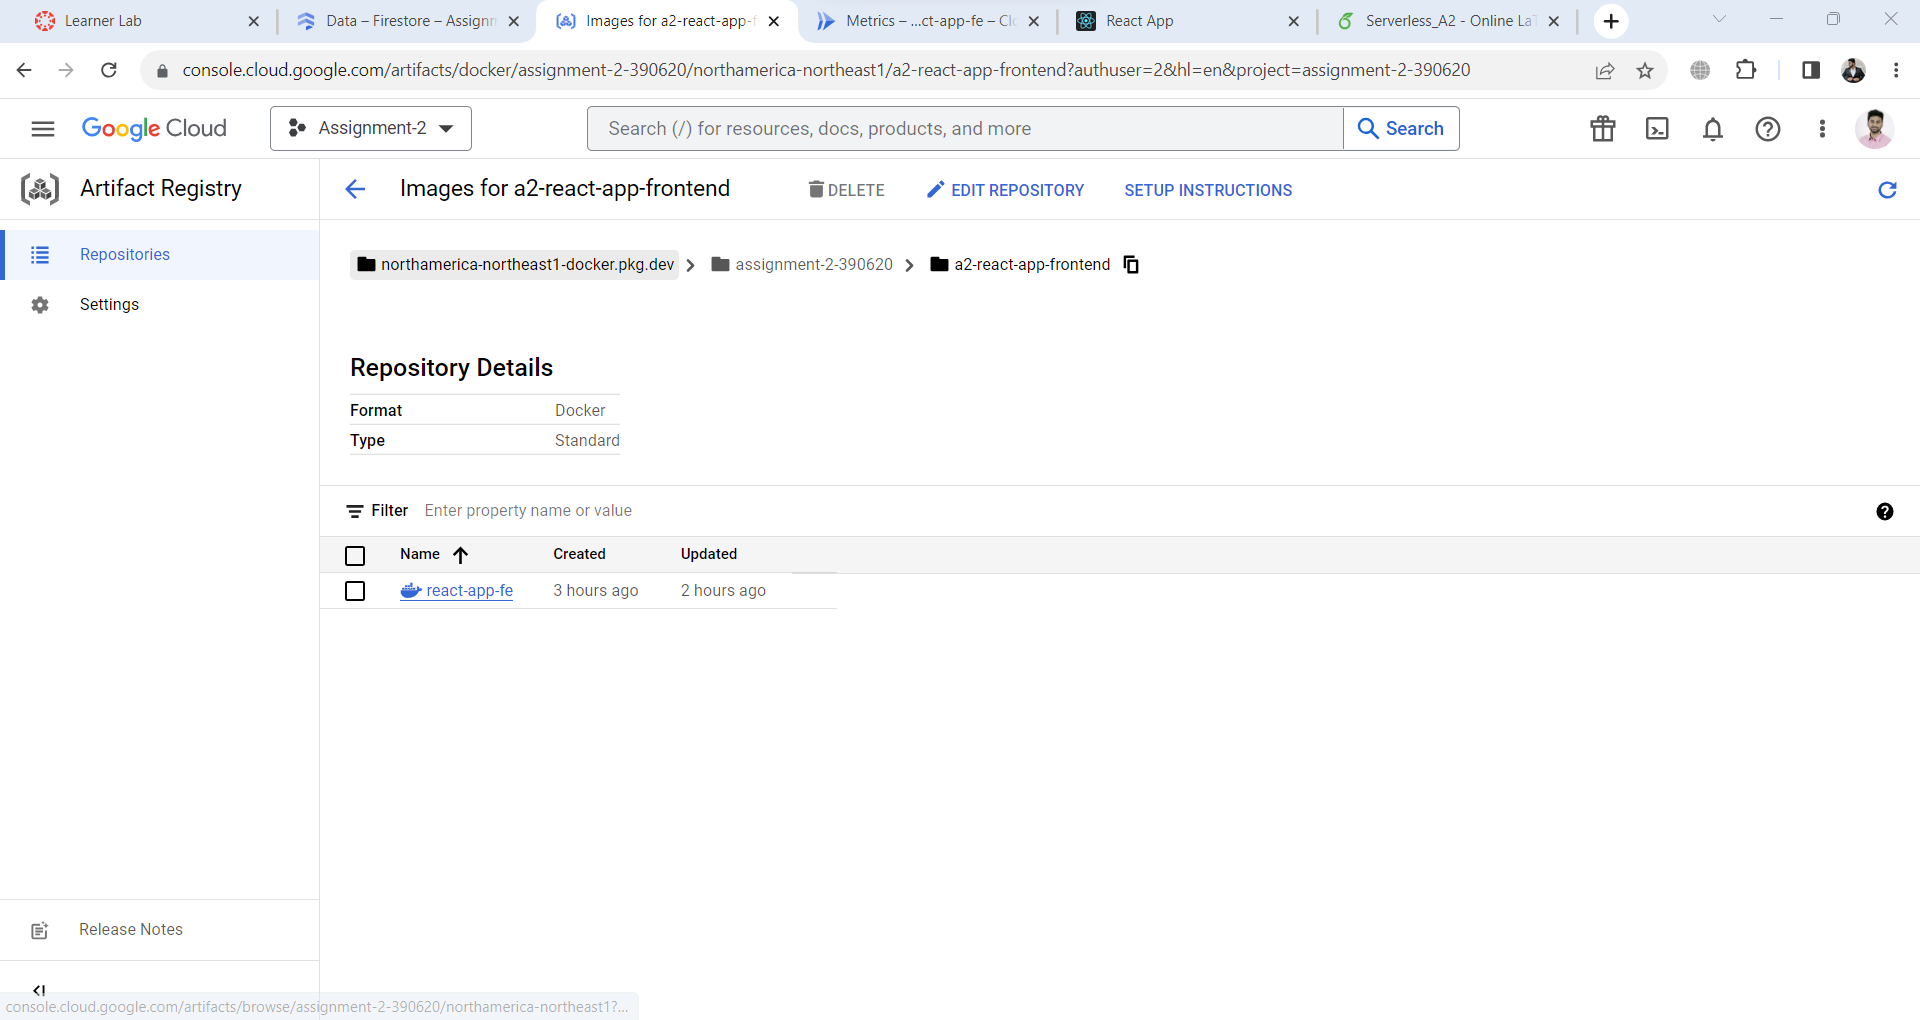
\includegraphics[scale=1, width=15cm,height=7.5cm]{PROBLEM 2/Screenshots/1. Setup/2. artifact reg repos/4. react-fe image.png}}
    \caption{\textbf{\textit{ Artifact registry repository - react-app frontend container }}}
    \label{fig:Artifact-registry-repo-cntr-fe}
\end{figure}

\begin{figure}[htp]
    \centering
    \fbox{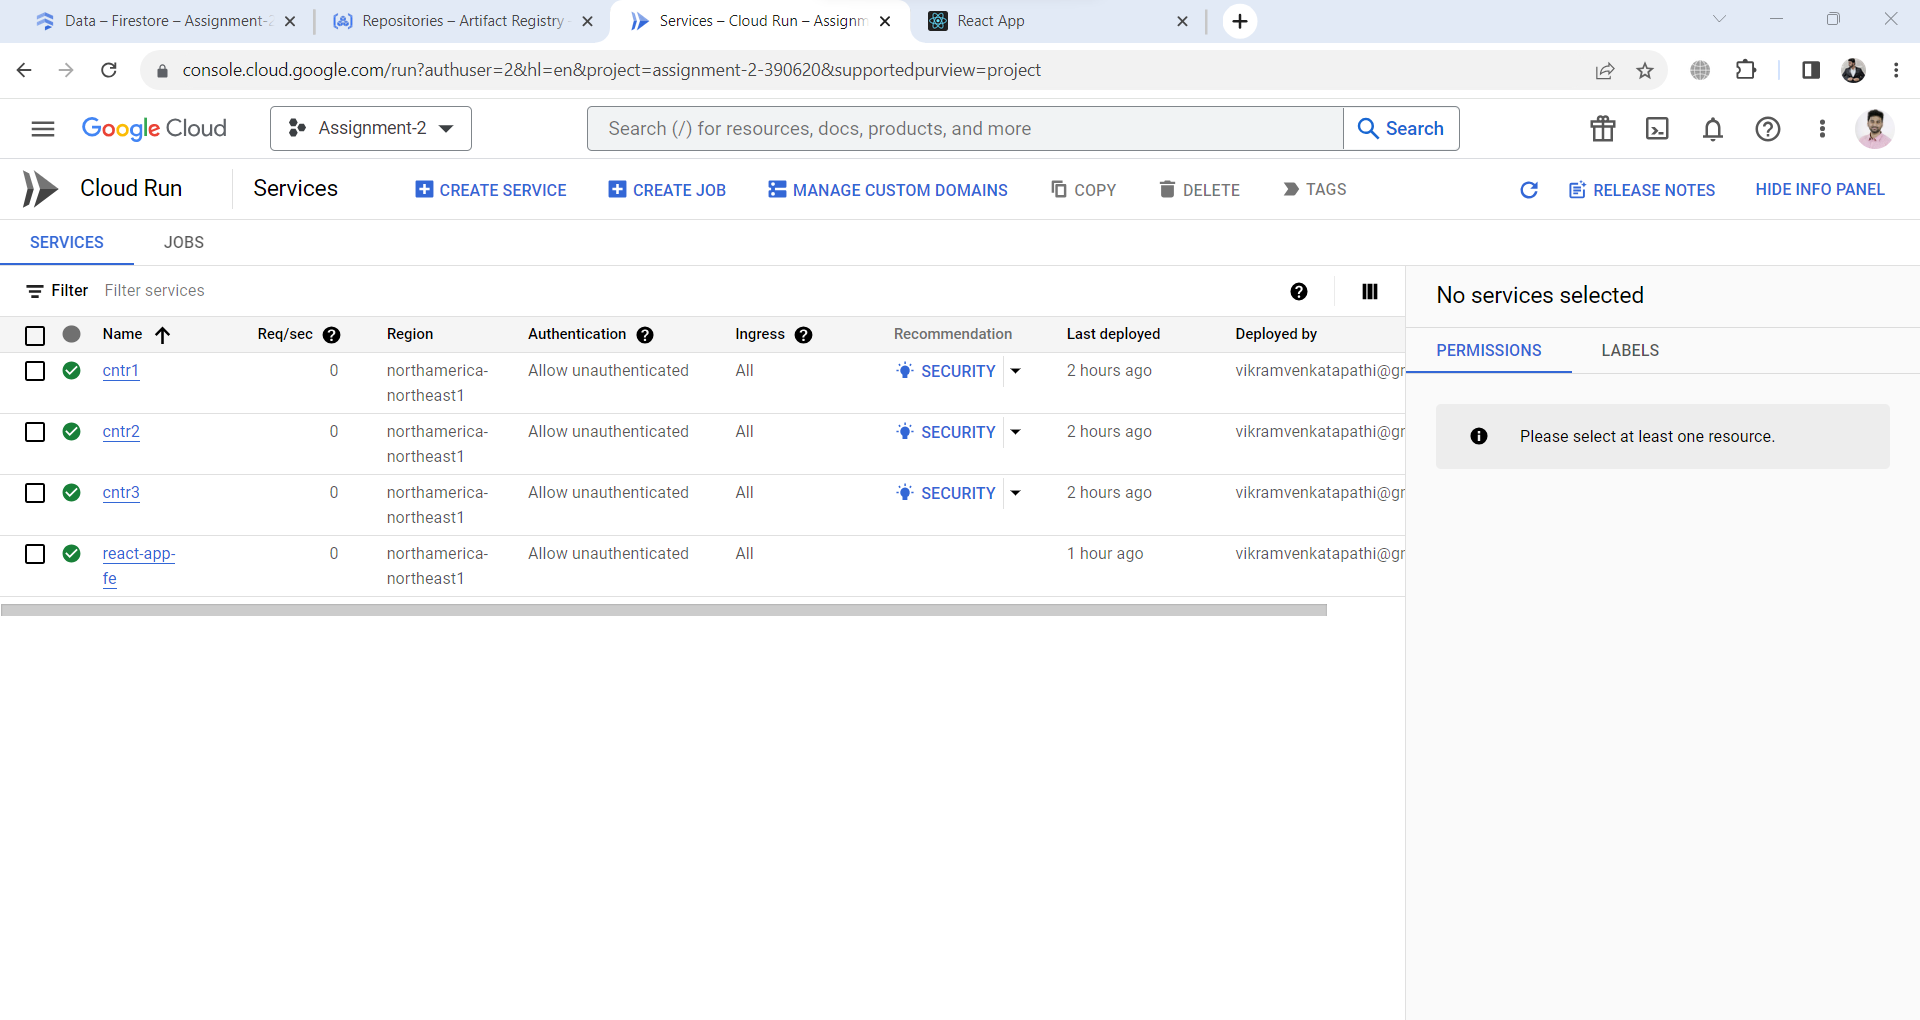
\includegraphics[scale=1, width=15cm,height=7.5cm]{PROBLEM 2/Screenshots/1. Setup/4. Cloud run - services.png}}
    \caption{\textbf{\textit{ Services created in Cloud Run }}}
    \label{fig:Cloud-Run-services}
\end{figure}

\newpage
\section{Demo}
\textbf{NOTE:}
In some of the screenshots, the URLs displayed on the front end may vary due to the process of deleting and recreating services on Cloud Run. These changes were made during the documentation process, which resulted in different URLs being assigned to the deployed containers. Please note that despite the variations in the URLs shown in the screenshots, the overall functionality and deployment process remains consistent.
\begin{figure}[htp]
    \centering
    \fbox{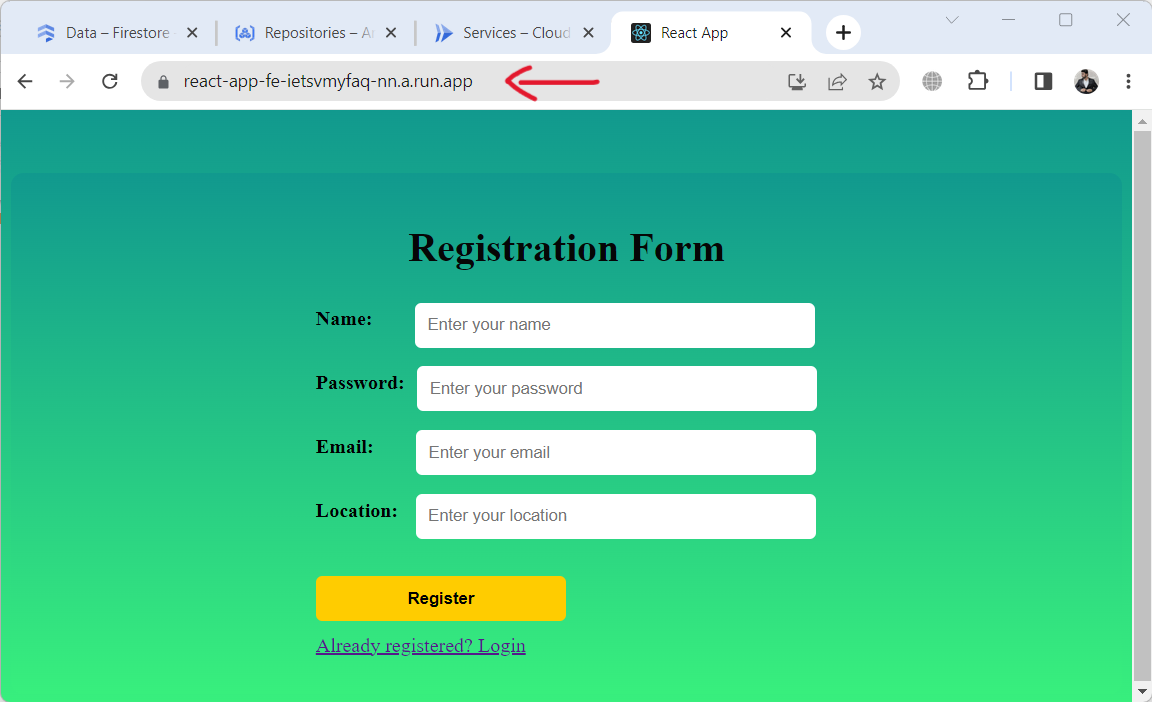
\includegraphics[scale=1, width=15cm,height=7.5cm]{PROBLEM 2/Screenshots/2. Demo/1. Reg. page.png}}
    \caption{\textbf{\textit{ Registration page }}}
    \label{fig:reg-page}
\end{figure}

\begin{figure}[htp]
    \centering
    \fbox{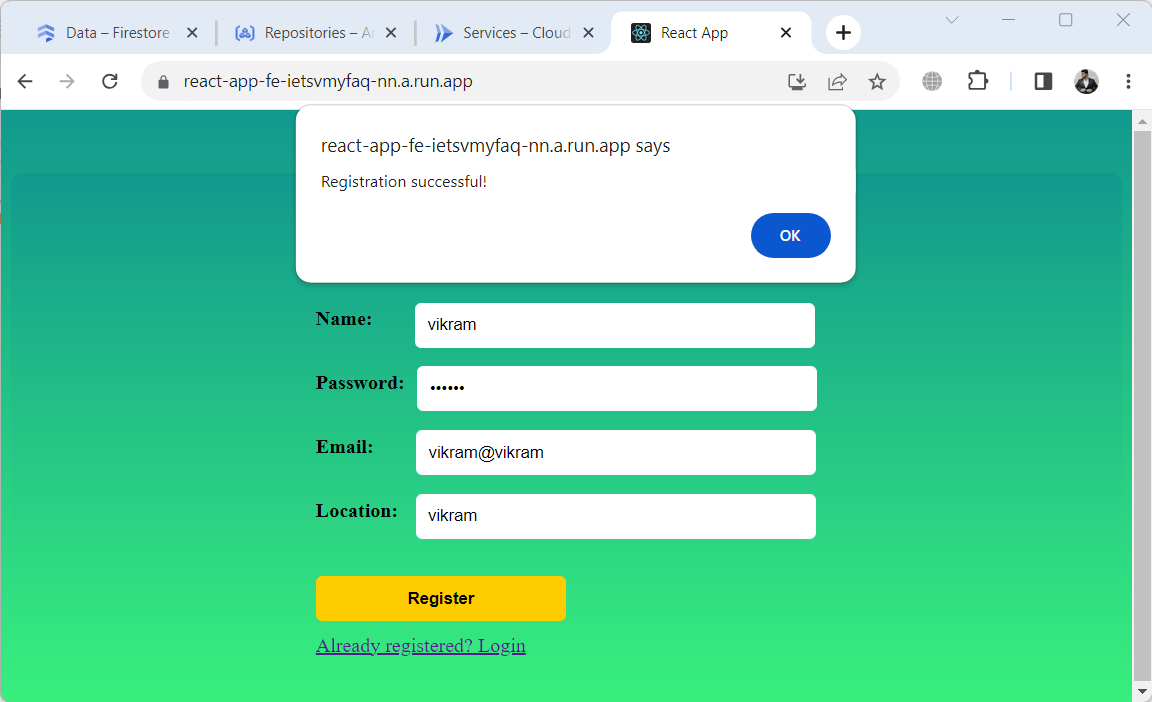
\includegraphics[scale=1, width=15cm,height=7.5cm]{PROBLEM 2/Screenshots/2. Demo/1.1 Reg success.png}}
    \caption{\textbf{\textit{ User - Vikram: Registration success }}}
    \label{fig:vikram-reg-success}
\end{figure}

\begin{figure}[htp]
    \centering
    \fbox{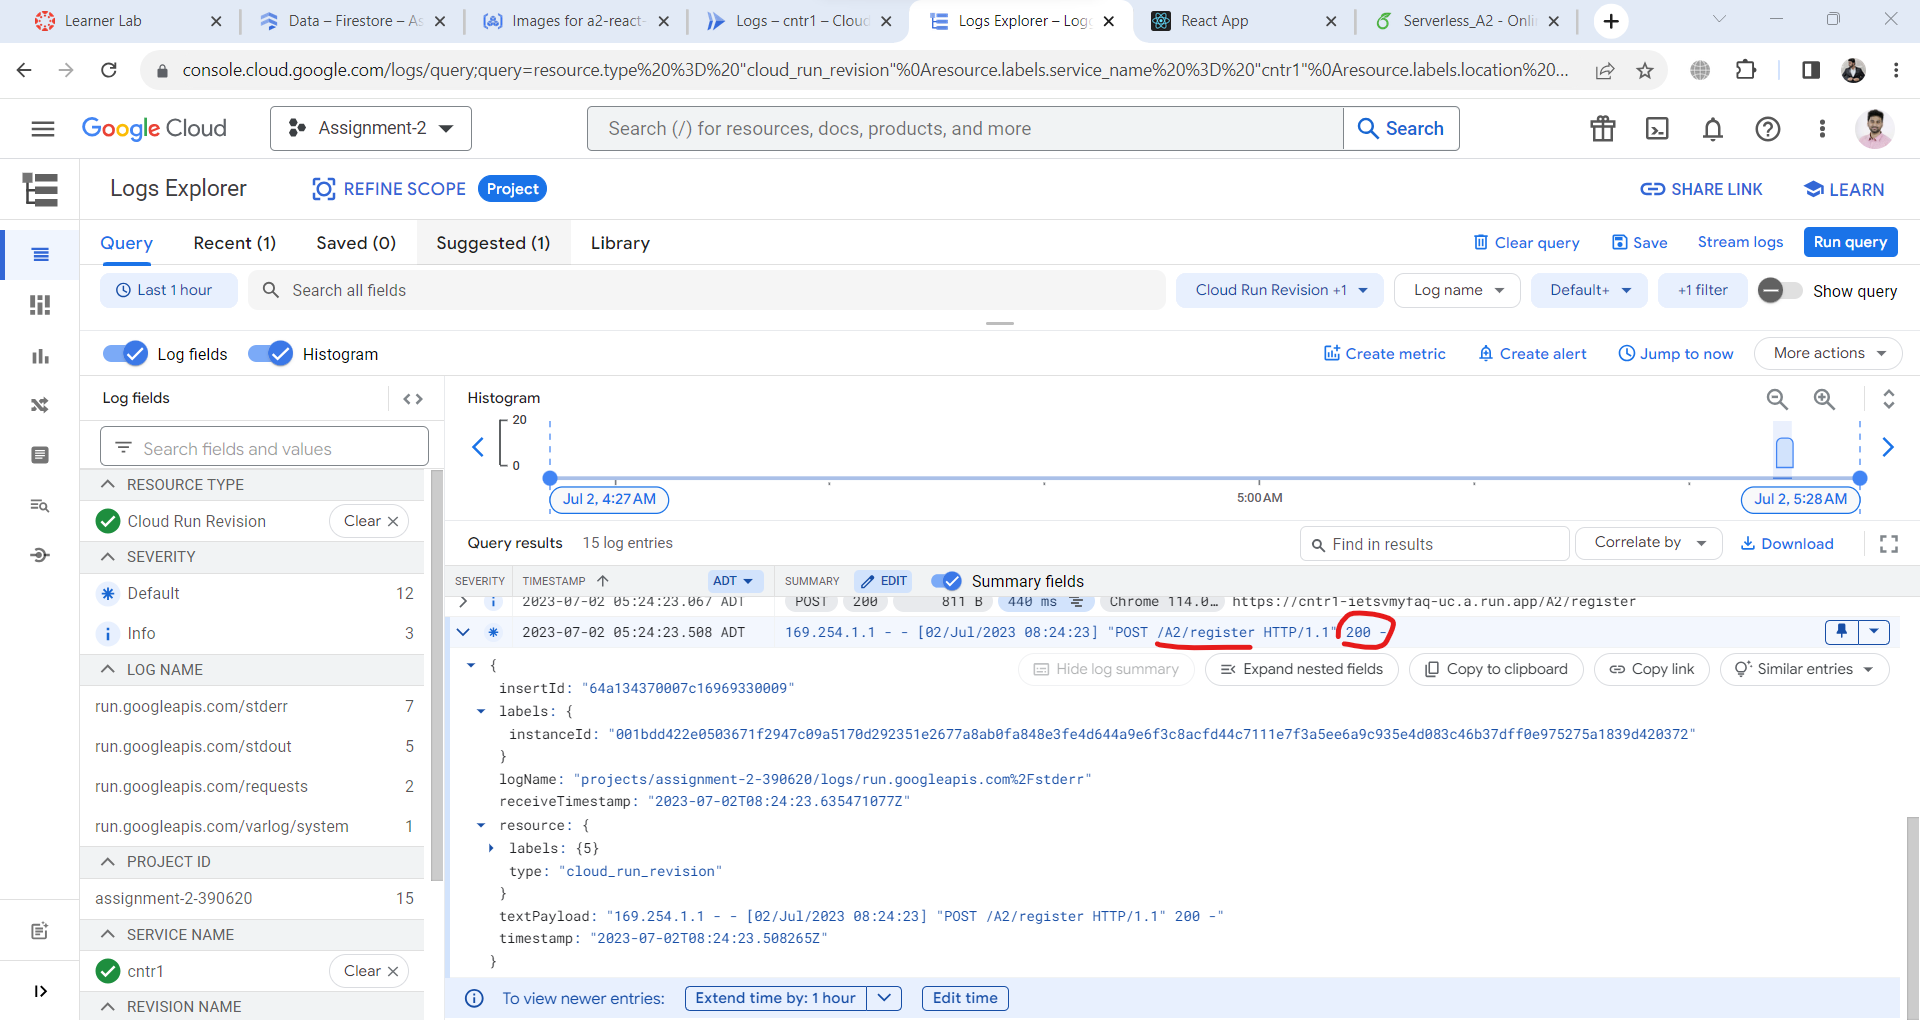
\includegraphics[scale=1, width=15cm,height=7.5cm]{PROBLEM 2/Screenshots/2. Demo/1. Logs/1. reg succes 200.png}}
    \caption{\textbf{\textit{ User - Vikram: Registration Logs}}}
    \label{fig:vikram-record-created}
\end{figure}

\begin{figure}[htp]
    \centering
    \fbox{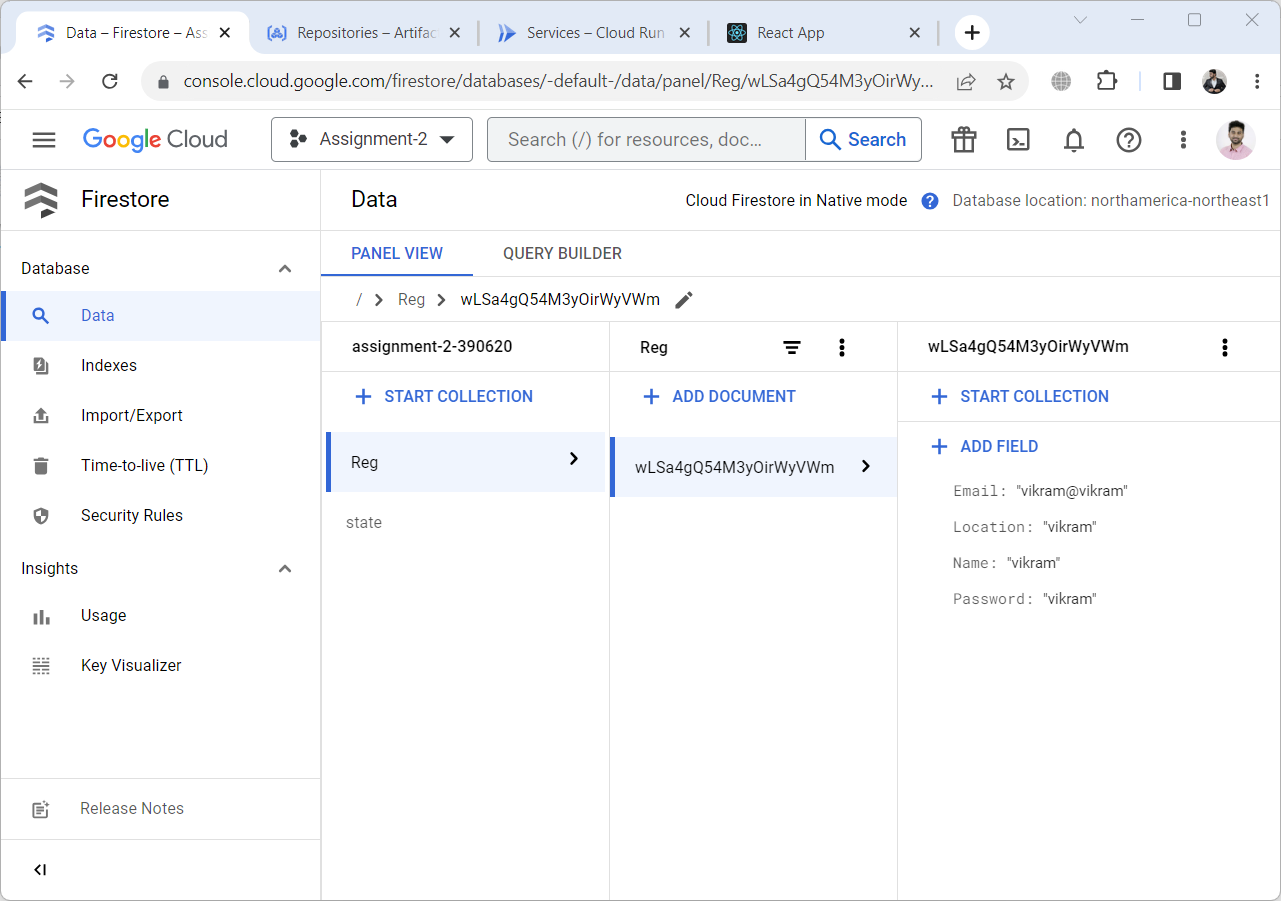
\includegraphics[scale=1, width=15cm,height=7.5cm]{PROBLEM 2/Screenshots/2. Demo/1.3 Vikram-record created.png}}
    \caption{\textbf{\textit{ User - Vikram: Document created in "Reg" }}}
    \label{fig:vikram-record-created}
\end{figure}


\begin{figure}[htp]
    \centering
    \fbox{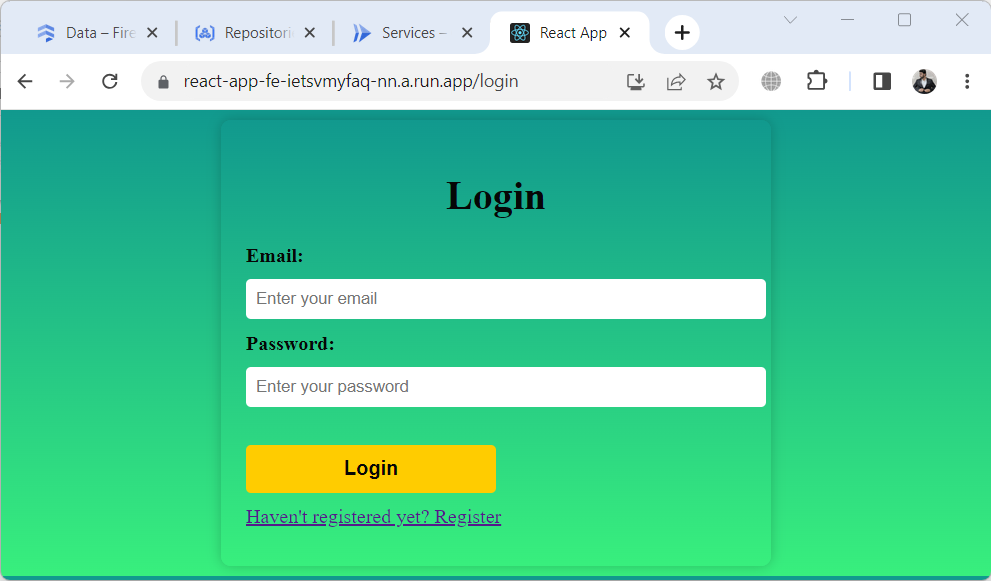
\includegraphics[scale=1, width=15cm,height=7.5cm]{PROBLEM 2/Screenshots/2. Demo/2. Login page.png}}
    \caption{\textbf{\textit{ Login page }}}
    \label{fig:login-page}
\end{figure}

\begin{figure}[htp]
    \centering
    \fbox{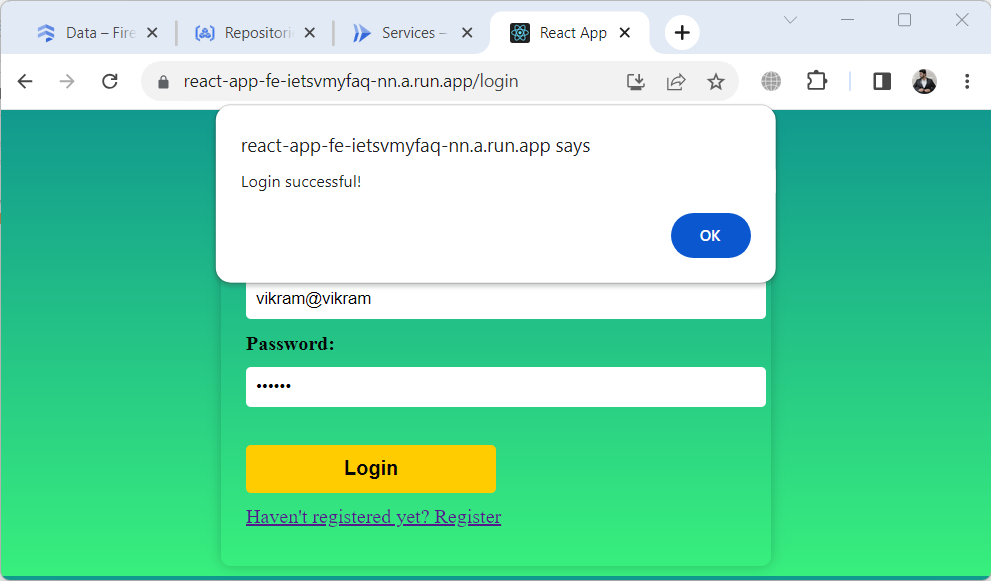
\includegraphics[scale=1, width=15cm,height=7.5cm]{PROBLEM 2/Screenshots/2. Demo/2.1 Login success.png}}
    \caption{\textbf{\textit{ User - Vikram: Login Success }}}
    \label{fig:vikram-login-success}
\end{figure}

\begin{figure}[htp]
    \centering
    \fbox{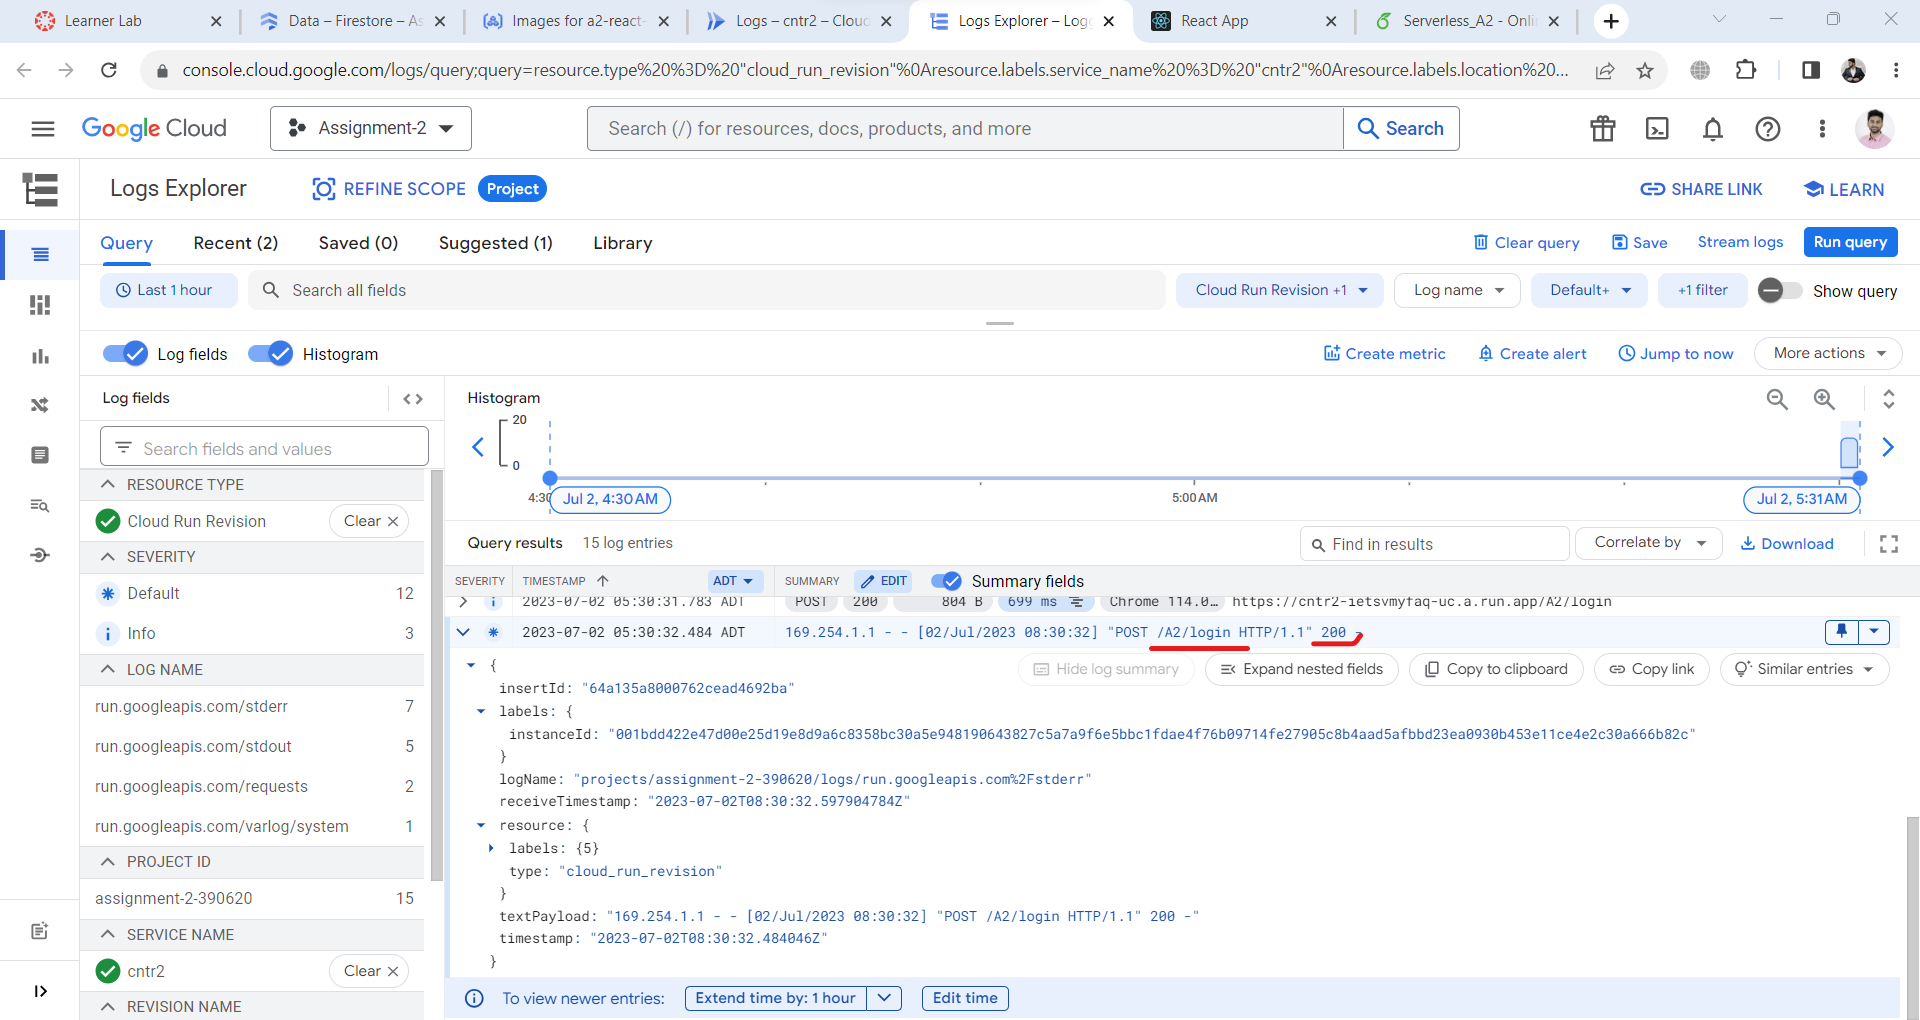
\includegraphics[scale=1, width=15cm,height=7.5cm]{PROBLEM 2/Screenshots/2. Demo/1. Logs/2. login success 200.png}}
    \caption{\textbf{\textit{ User - Vikram: Login logs }}}
    \label{fig:vikram-session-data-page}
\end{figure}

\begin{figure}[htp]
    \centering
    \fbox{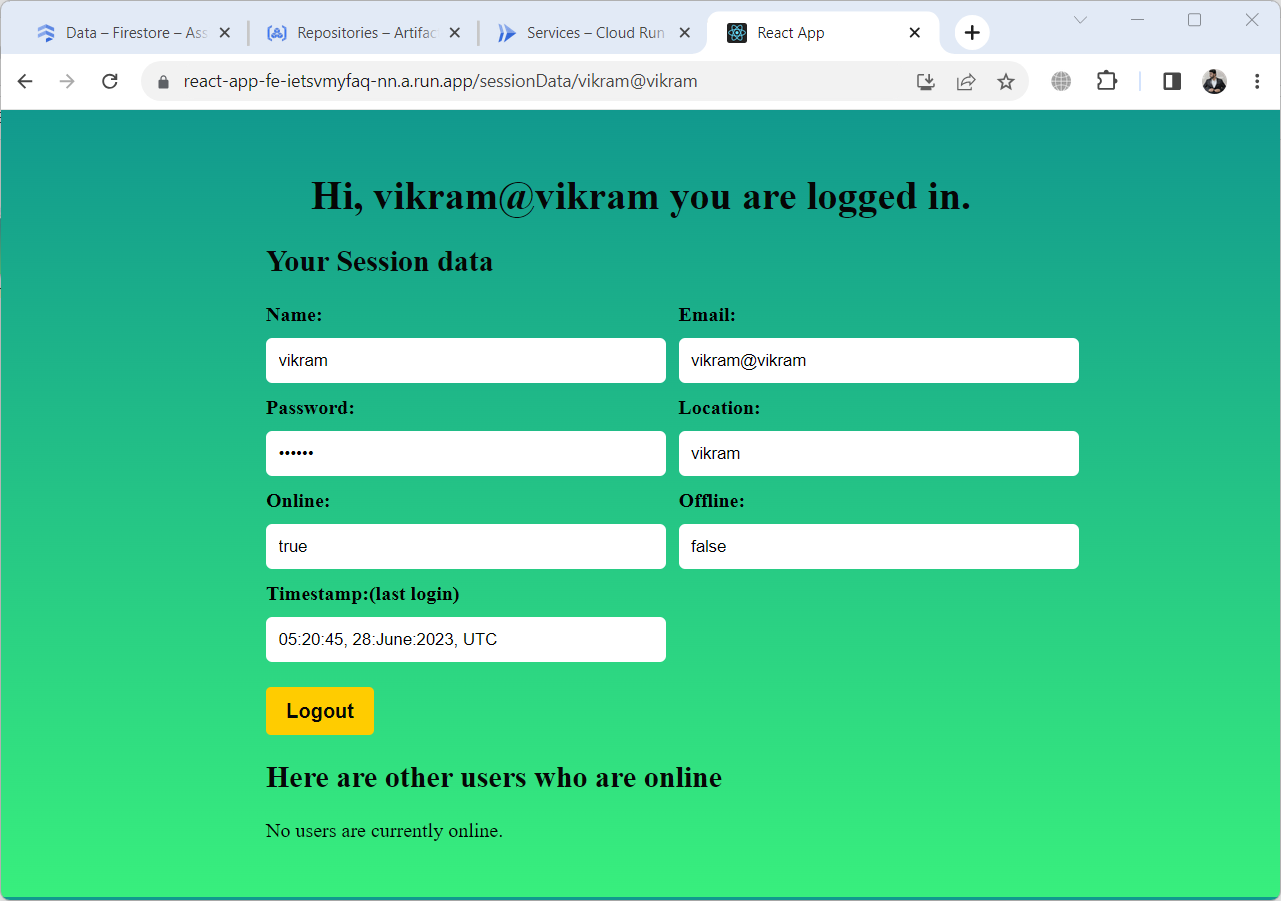
\includegraphics[scale=1, width=15cm,height=7.5cm]{PROBLEM 2/Screenshots/2. Demo/3.1 Session data for vikram.png}}
    \caption{\textbf{\textit{ User - Vikram: Session data page (no other users online) }}}
    \label{fig:vikram-session-data-page}
\end{figure}

\begin{figure}[htp]
    \centering
    \fbox{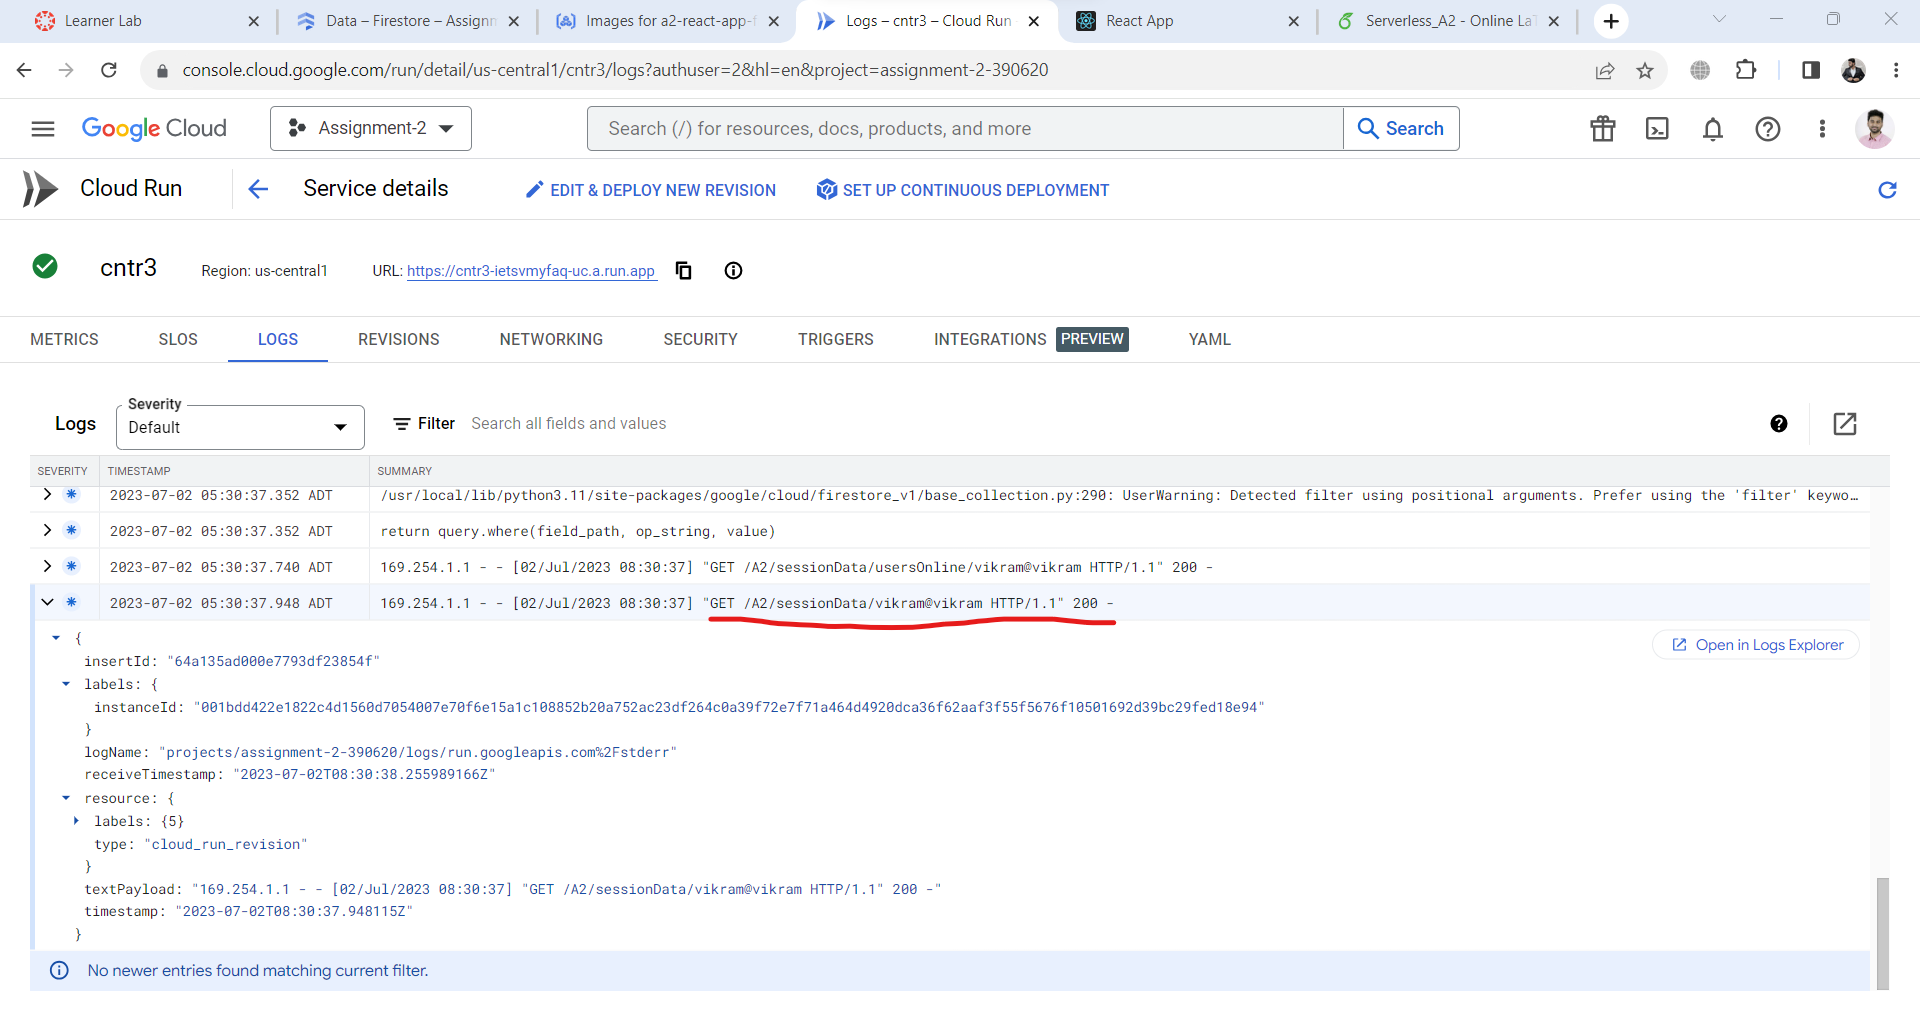
\includegraphics[scale=1, width=15cm,height=7.5cm]{PROBLEM 2/Screenshots/2. Demo/1. Logs/3. session vikram showing.png}}
    \caption{\textbf{\textit{ User - Vikram: session logs }}}
    \label{fig:vikram-session-data-page}
\end{figure}

\begin{figure}[htp]
    \centering
    \fbox{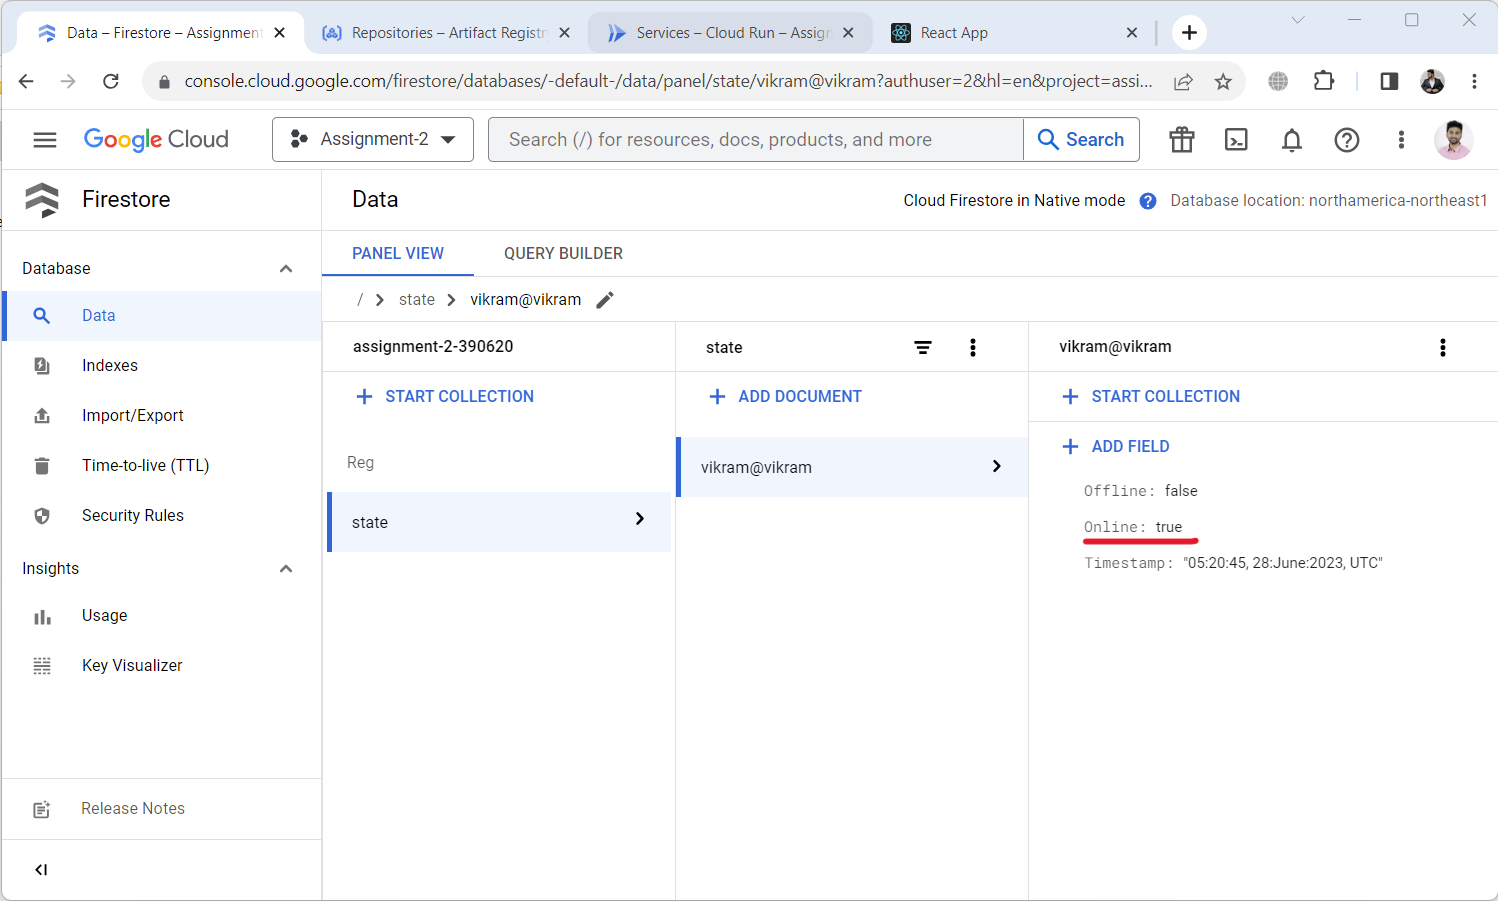
\includegraphics[scale=1, width=15cm,height=7.5cm]{PROBLEM 2/Screenshots/2. Demo/3.2 vikram - after login - online.png}}
    \caption{\textbf{\textit{ User - Vikram: Session data document in "state"}}}
    \label{fig:vikram-session-data-document}
\end{figure}

\begin{figure}[htp]
    \centering
    \fbox{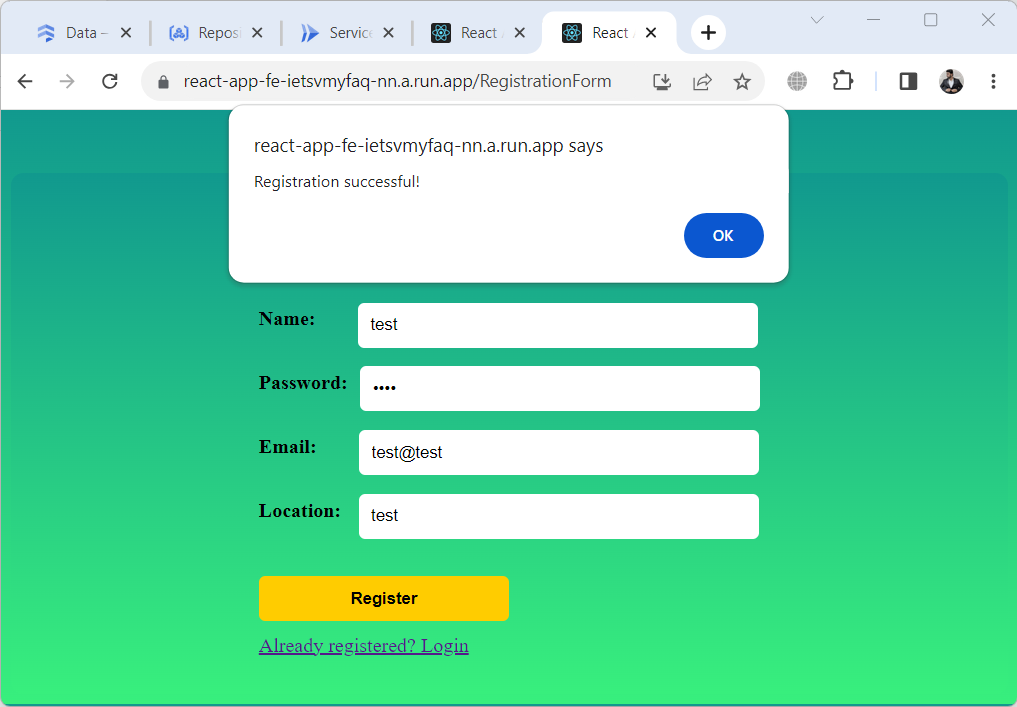
\includegraphics[scale=1, width=15cm,height=7.5cm]{PROBLEM 2/Screenshots/2. Demo/4.1 test- reg success.png}}
    \caption{\textbf{\textit{ User - test: Registration success}}}
    \label{fig:test-reg-success}
\end{figure}

\begin{figure}[htp]
    \centering
    \fbox{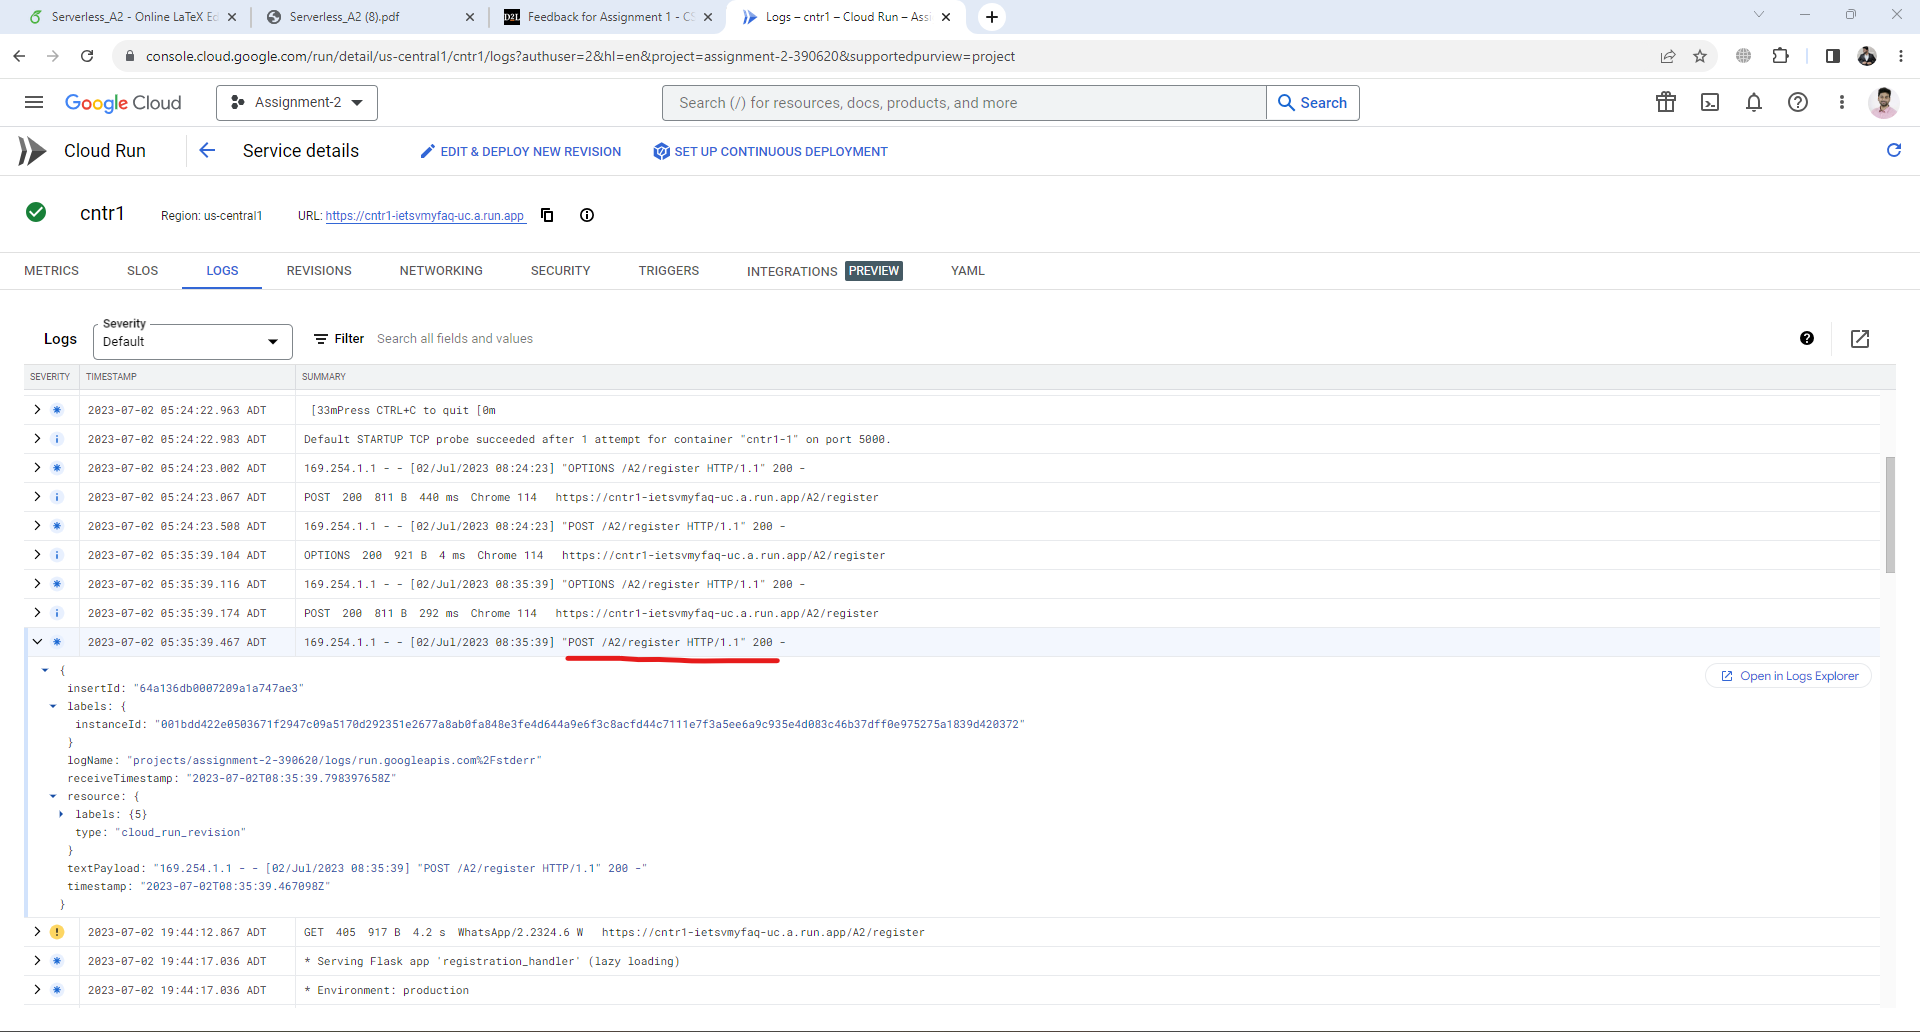
\includegraphics[scale=1, width=15cm,height=7.5cm]{PROBLEM 2/Screenshots/2. Demo/1. Logs/1.1 test reg success.png}}
    \caption{\textbf{\textit{ User - test: Registration success logs}}}
    \label{fig:test-reg-success}
\end{figure}

\begin{figure}[htp]
    \centering
    \fbox{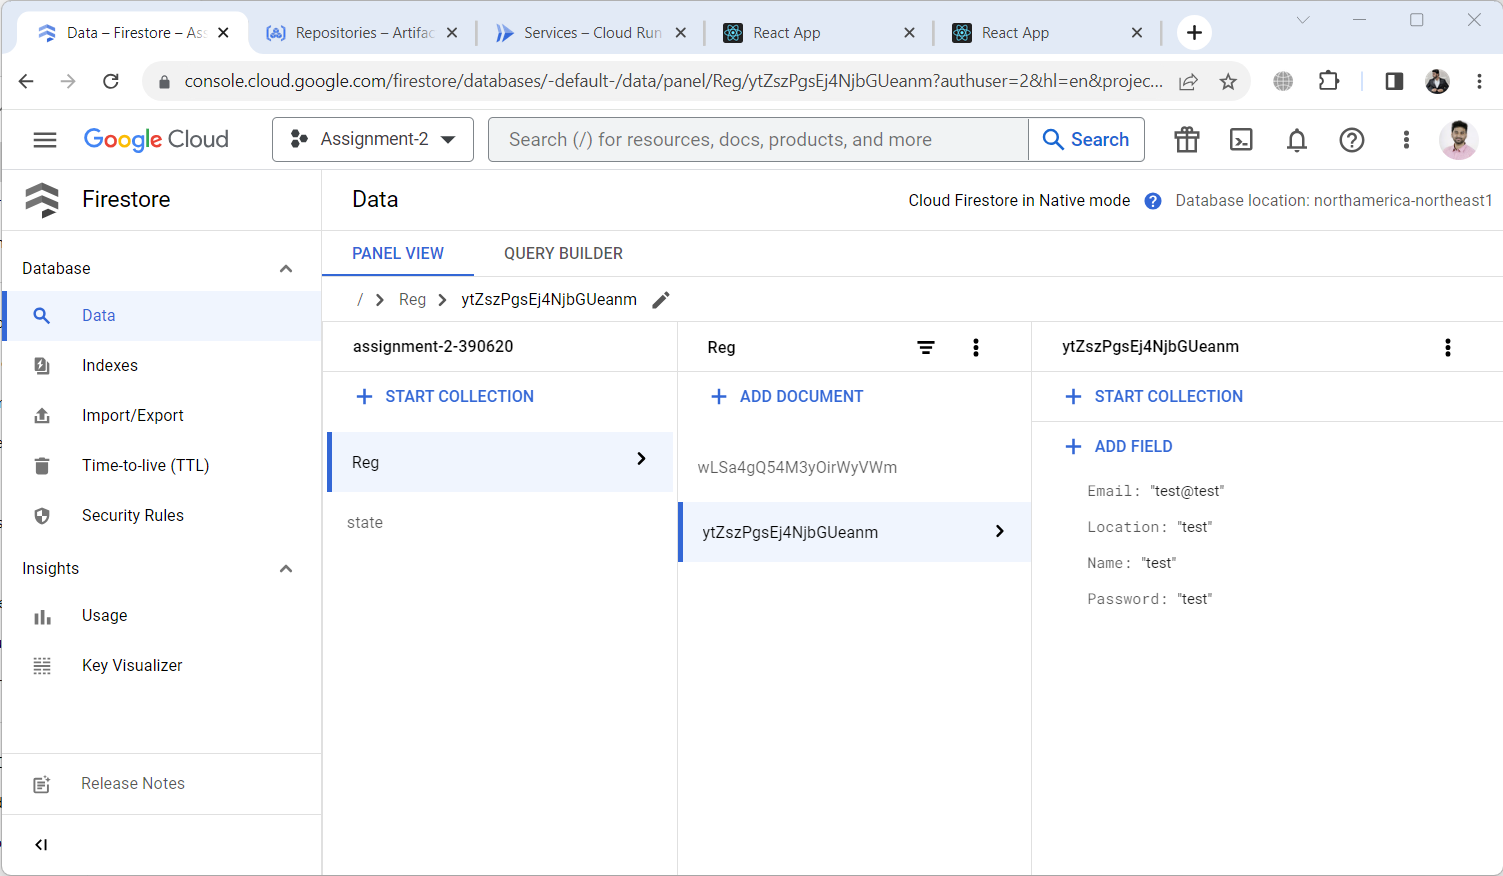
\includegraphics[scale=1, width=15cm,height=7.5cm]{PROBLEM 2/Screenshots/2. Demo/4.2 test record created in Reg.png}}
    \caption{\textbf{\textit{ User - test: document created in "Reg"}}}
    \label{fig:test-record-created-reg}
\end{figure}

\begin{figure}[htp]
    \centering
    \fbox{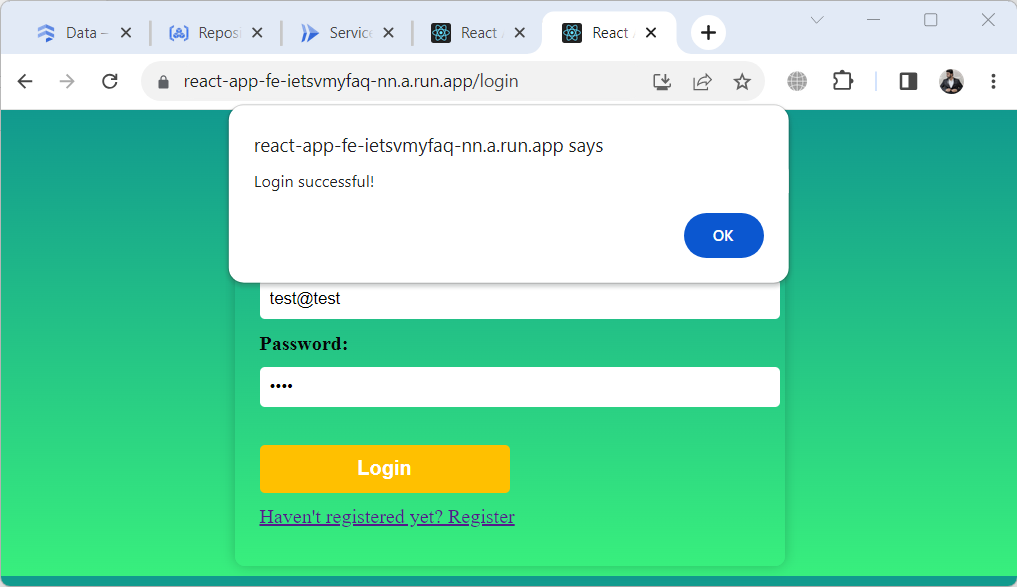
\includegraphics[scale=1, width=15cm,height=7.5cm]{PROBLEM 2/Screenshots/2. Demo/4.3 test- login success.png}}
    \caption{\textbf{\textit{ User - test: Login success }}}
    \label{fig:test-login-success}
\end{figure}

\begin{figure}[htp]
    \centering
    \fbox{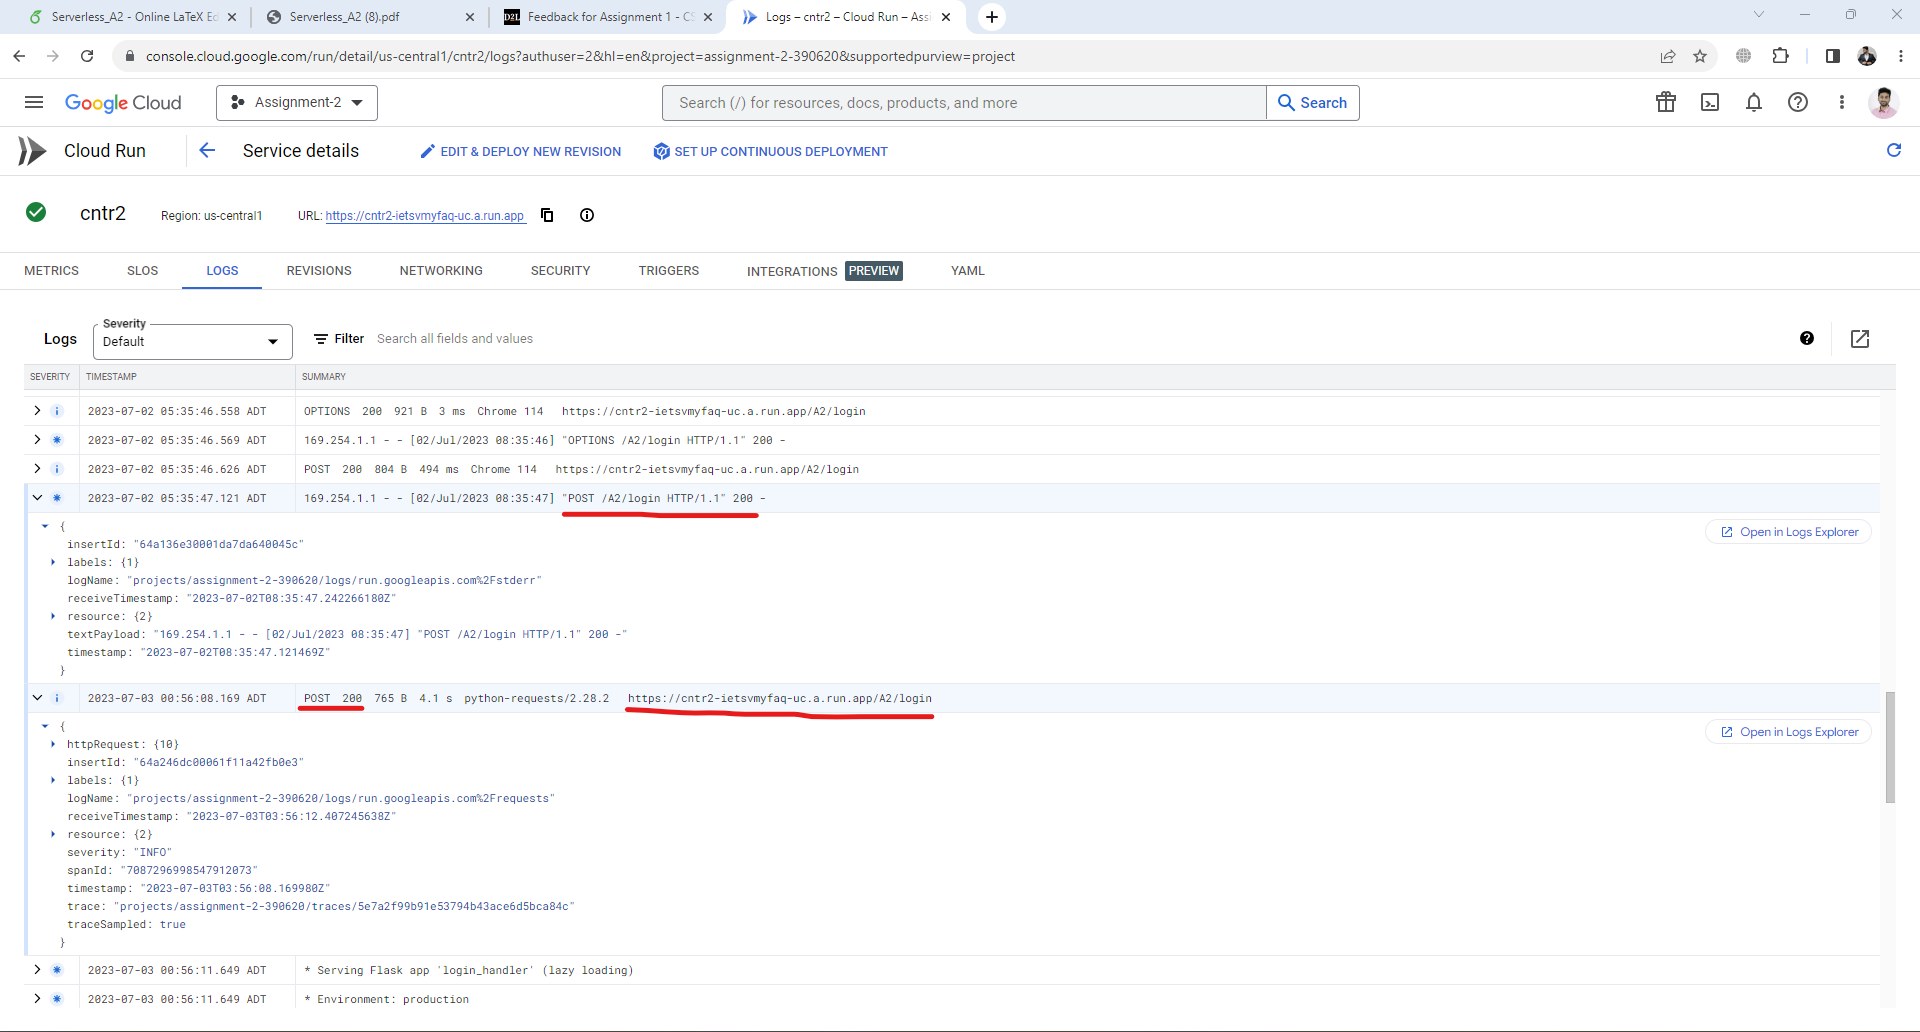
\includegraphics[scale=1, width=15cm,height=7.5cm]{PROBLEM 2/Screenshots/2. Demo/1. Logs/2.2 test login success.png}}
    \caption{\textbf{\textit{ User - test: Login success logs}}}
    \label{fig:test-login-success}
\end{figure}

\begin{figure}[htp]
    \centering
    \fbox{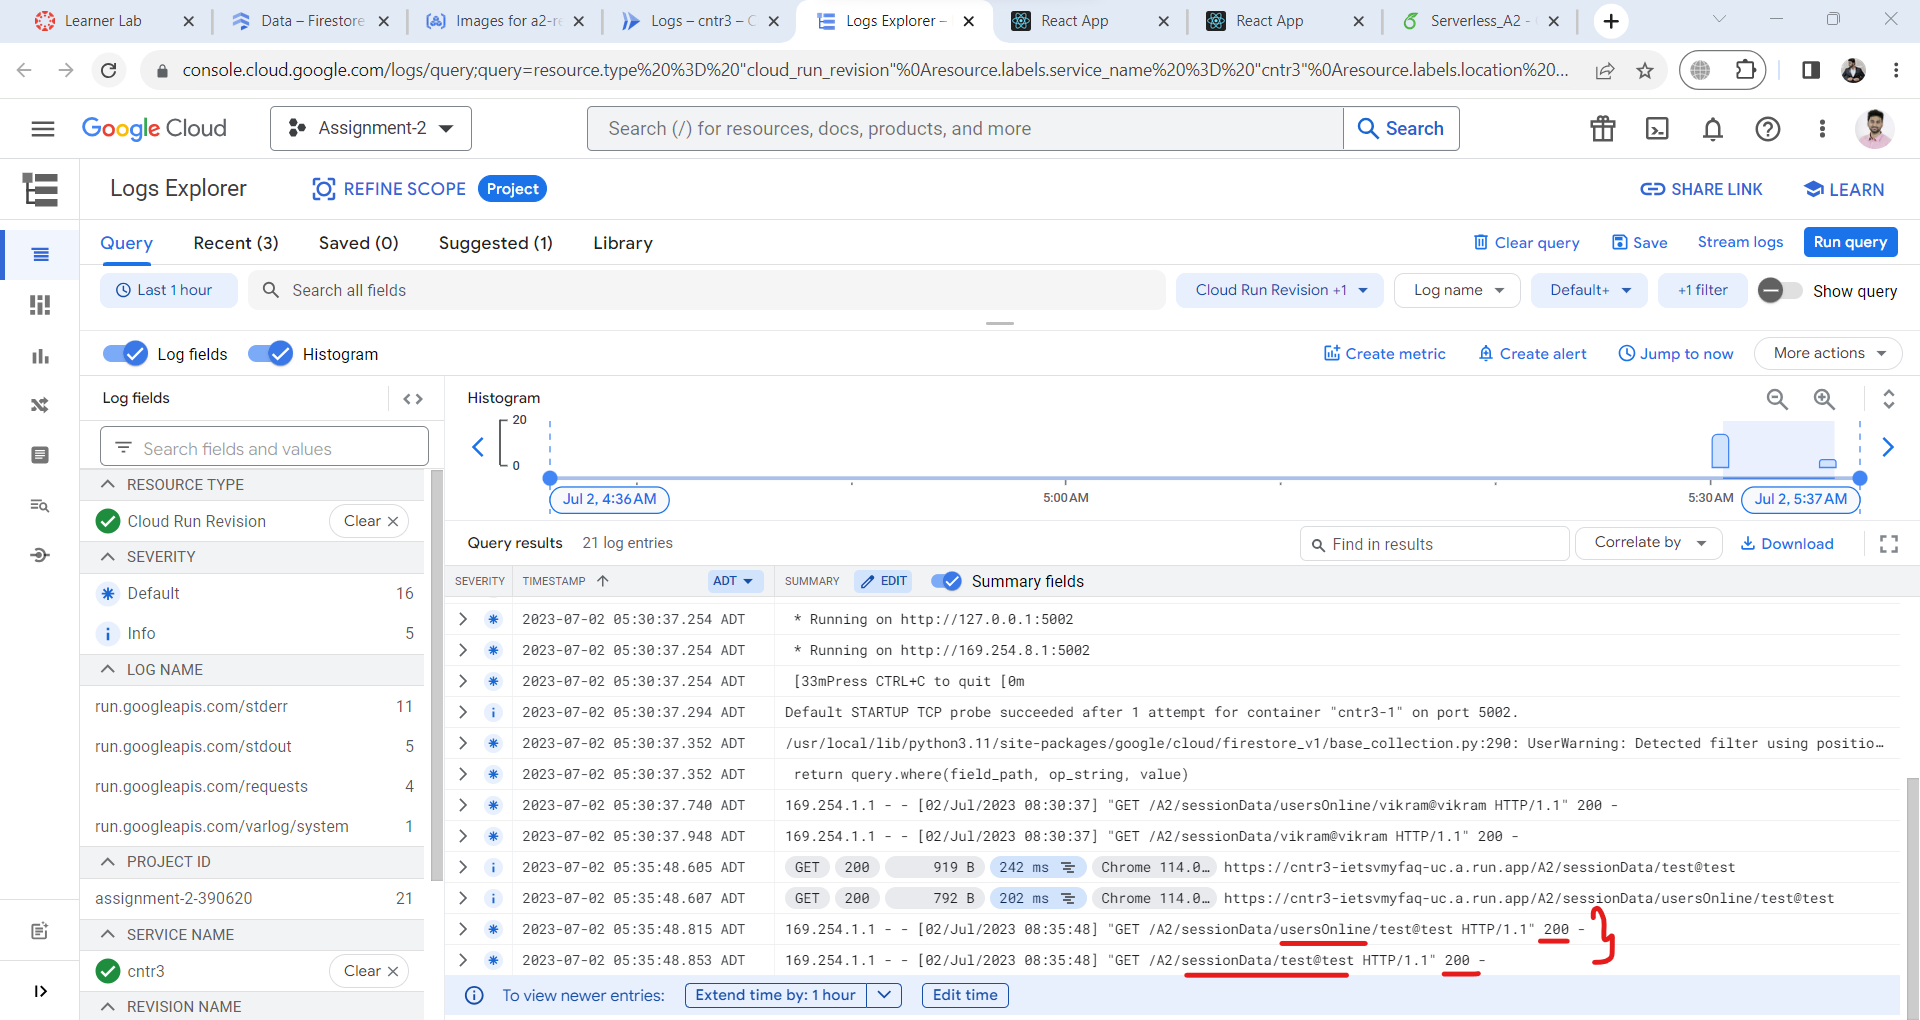
\includegraphics[scale=1, width=15cm,height=7.5cm]{PROBLEM 2/Screenshots/2. Demo/1. Logs/3. session test showing .png}}
    \caption{\textbf{\textit{ User - test: Session data logs }}}
    \label{fig:test-login-success}
\end{figure}

\begin{figure}[htp]
    \centering
    \fbox{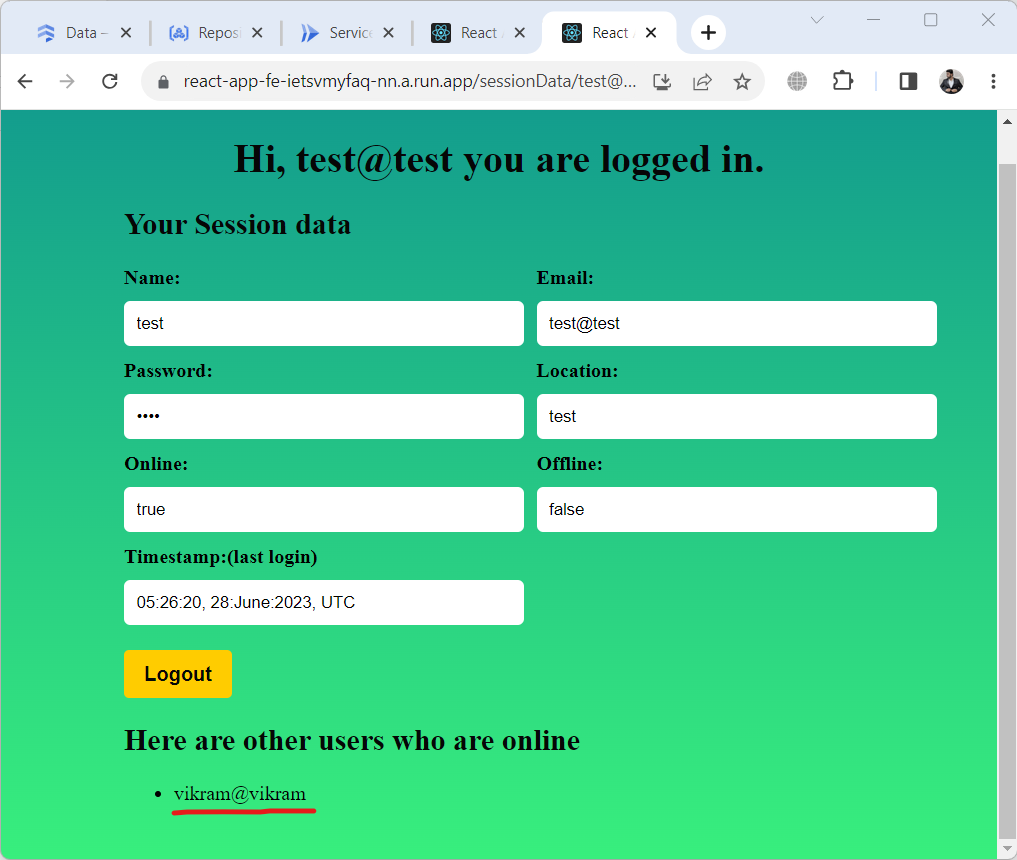
\includegraphics[scale=1, width=15cm,height=7.5cm]{PROBLEM 2/Screenshots/2. Demo/5.1 test session data - vikram online displaying.png}}
    \caption{\textbf{\textit{ User - test: session data (other online user(s) - "Vikram" is displaying) }}}
    \label{fig:test-session-data}
\end{figure}

\begin{figure}[htp]
    \centering
    \fbox{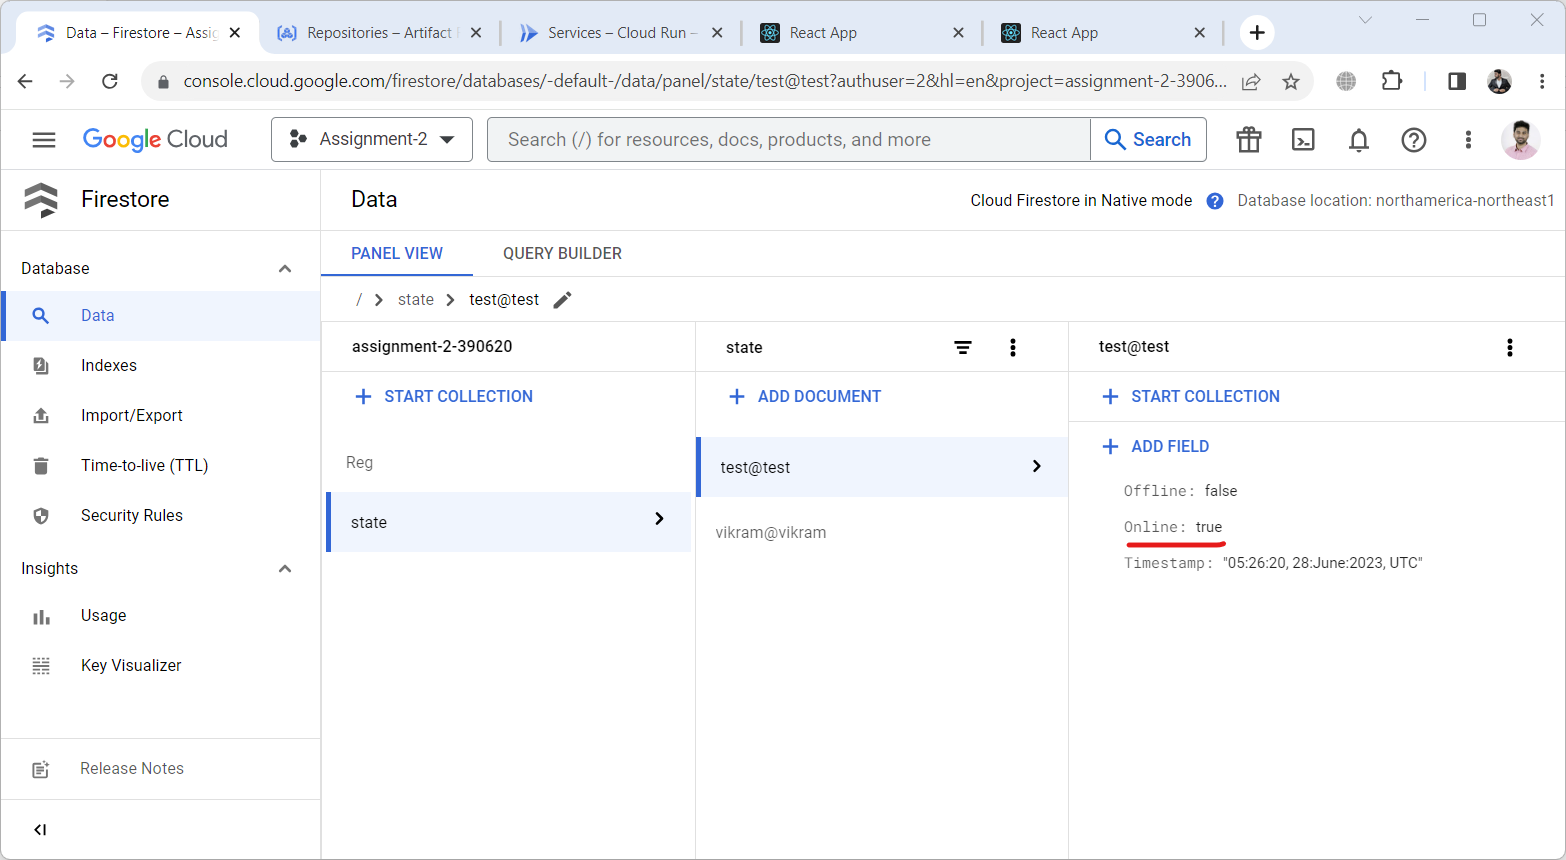
\includegraphics[scale=1, width=15cm,height=7.5cm]{PROBLEM 2/Screenshots/2. Demo/4.4 test after login - online.png}}
    \caption{\textbf{\textit{ User - test: document created in "state" }}}
    \label{fig:test-record-created-state}
\end{figure}



\begin{figure}[htp]
    \centering
    \fbox{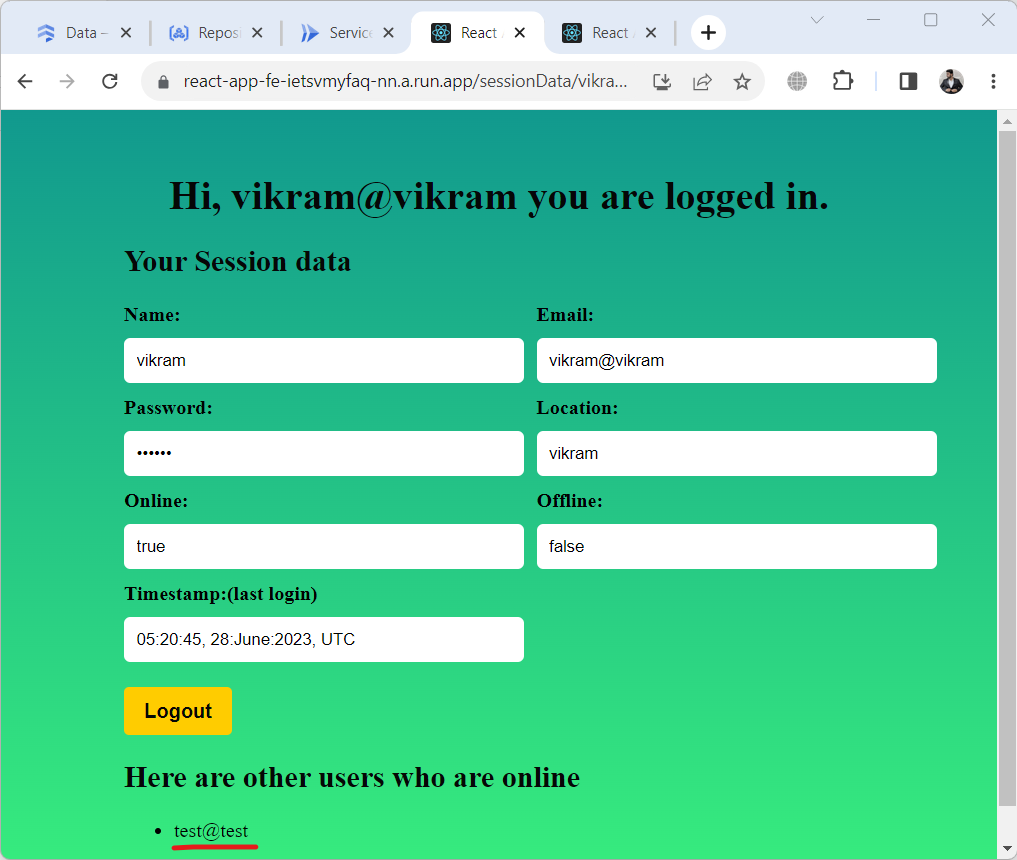
\includegraphics[scale=1, width=15cm,height=7.5cm]{PROBLEM 2/Screenshots/2. Demo/5.2 vikram session - test online displaying after refresh.png}}
    \caption{\textbf{\textit{ User - Vikram: session data (other online user(s) - "test" is displaying after refreshing the page) }}}
    \label{fig:vikram-session-data-refresh}
\end{figure}

\begin{figure}[htp]
    \centering
    \fbox{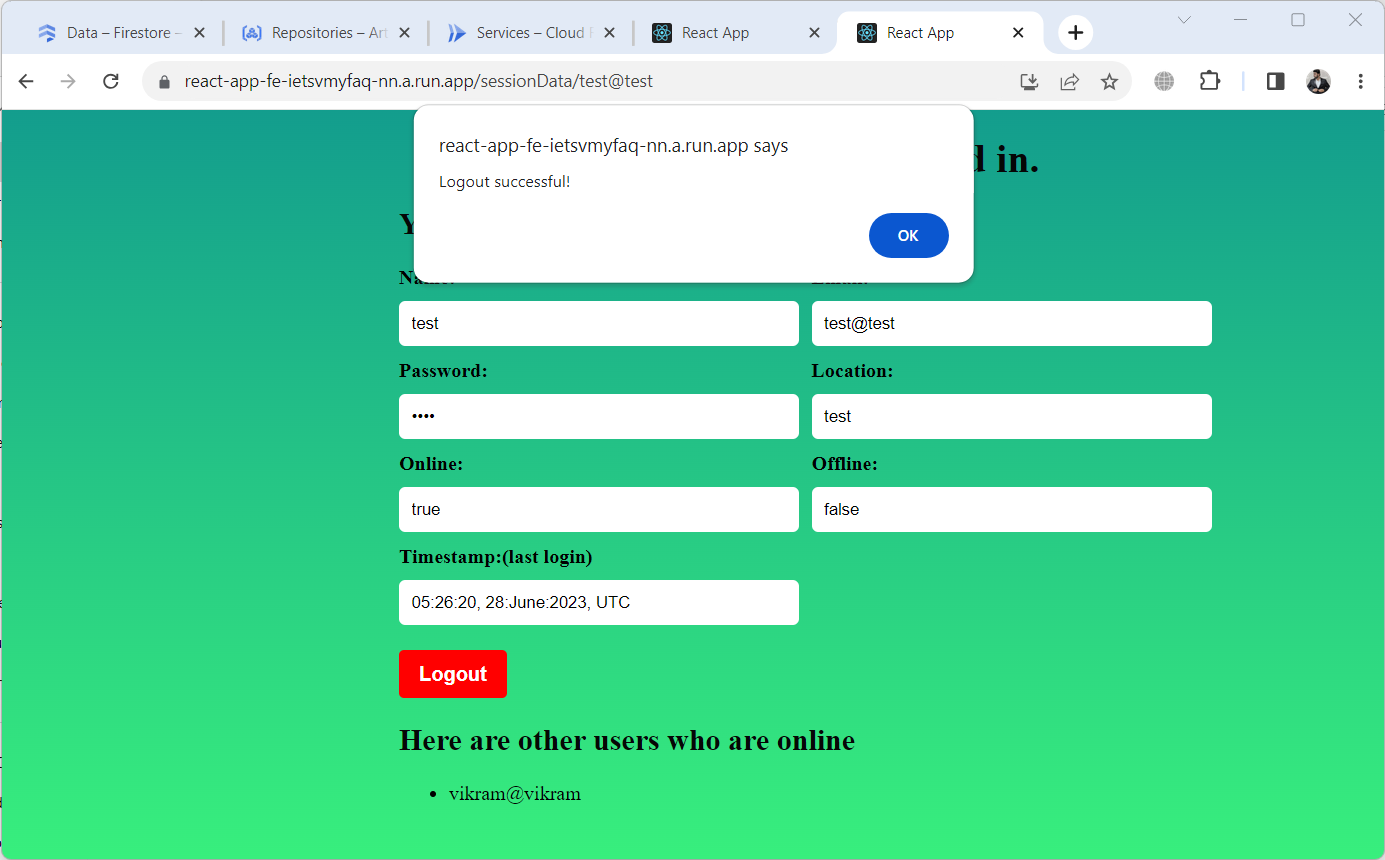
\includegraphics[scale=1, width=15cm,height=7.5cm]{PROBLEM 2/Screenshots/2. Demo/6.1 test - logout success.png}}
    \caption{\textbf{\textit{ User - test: Logout success }}}
    \label{fig:test-logout-success}
\end{figure}

\begin{figure}[htp]
    \centering
    \fbox{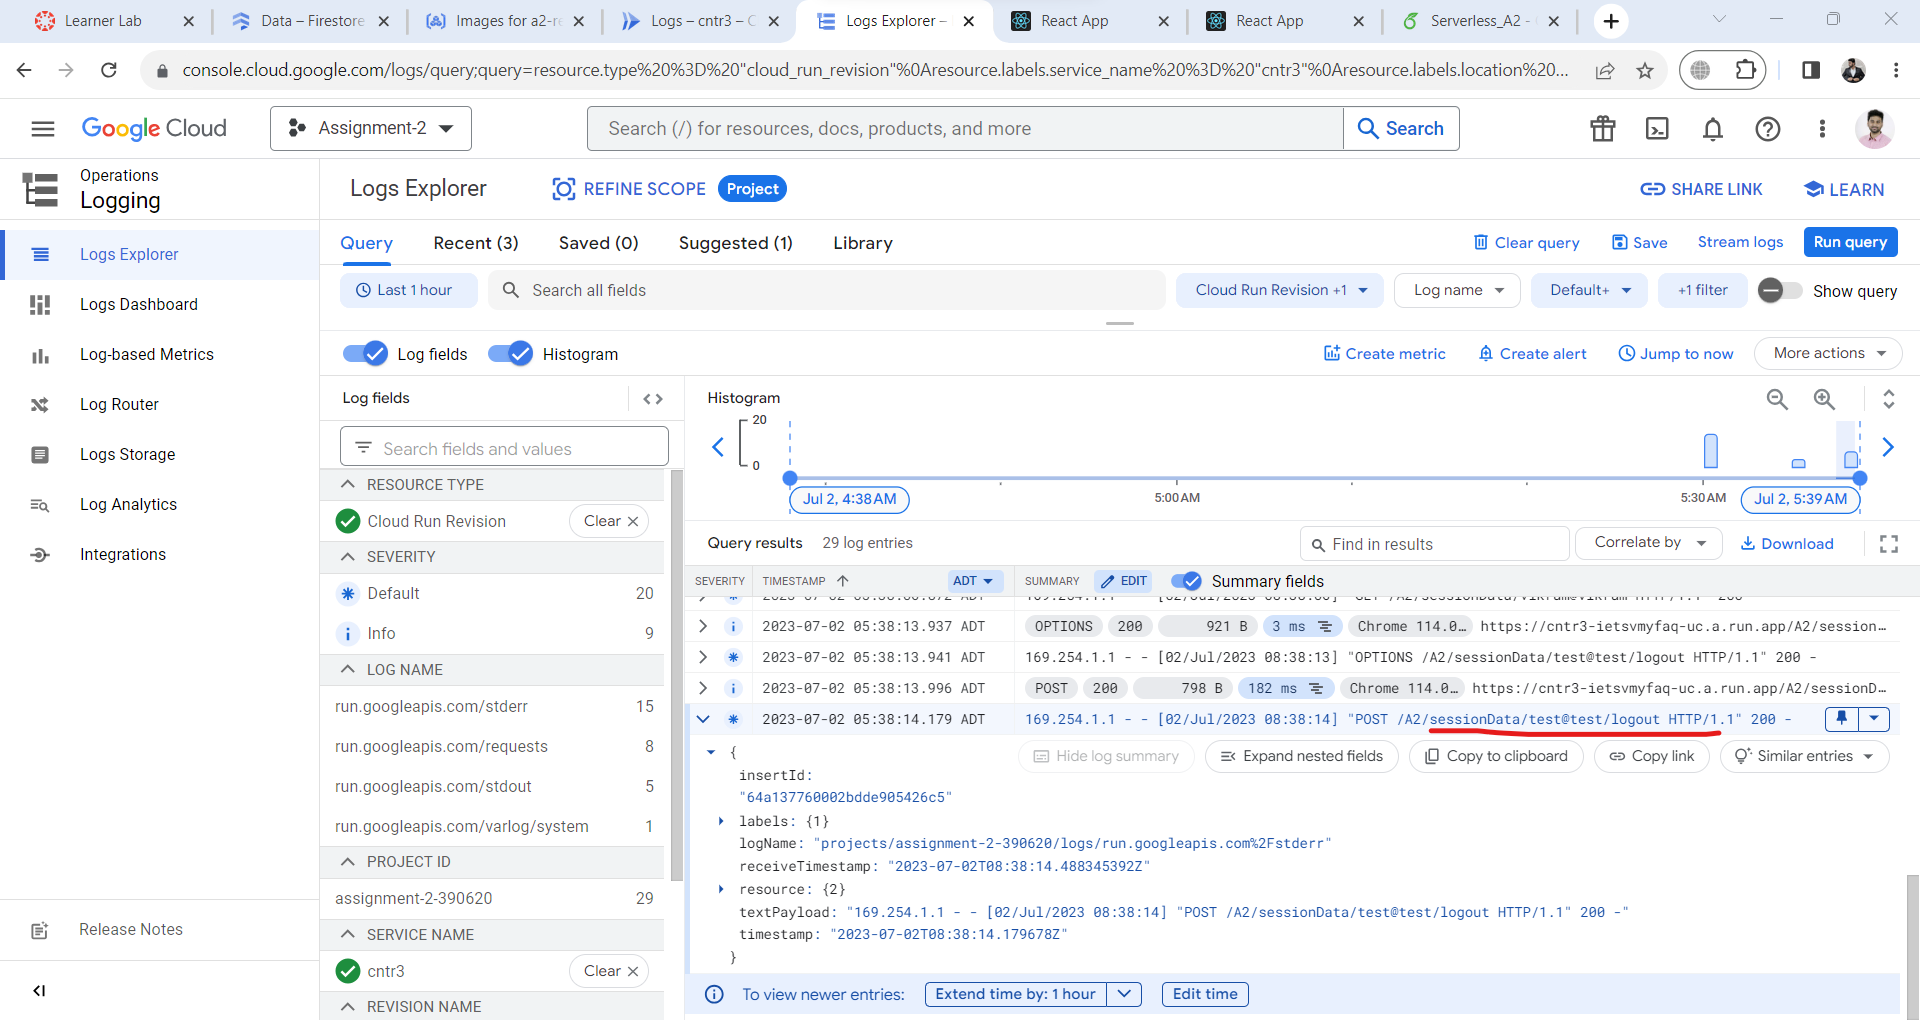
\includegraphics[scale=1, width=15cm,height=7.5cm]{PROBLEM 2/Screenshots/2. Demo/1. Logs/4. test session logout.png}}
    \caption{\textbf{\textit{ User - test: Logout logs }}}
    \label{fig:test-logout-success}
\end{figure}

\begin{figure}[htp]
    \centering
    \fbox{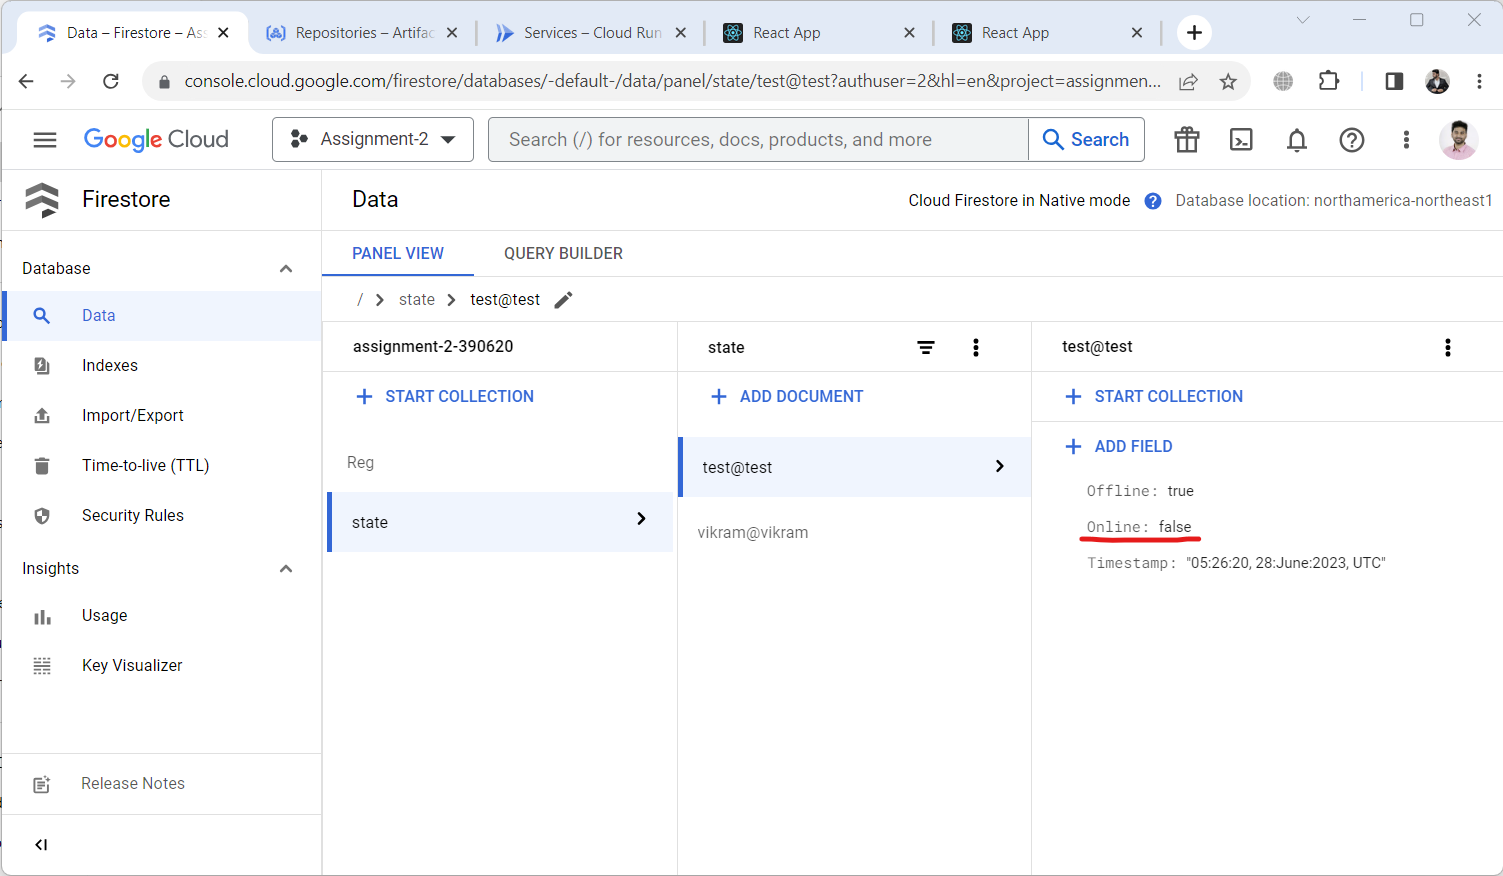
\includegraphics[scale=1, width=15cm,height=7.5cm]{PROBLEM 2/Screenshots/2. Demo/6.2 test session - offline after logout.png}}
    \caption{\textbf{\textit{ User - test: Session is Offline }}}
    \label{fig:test-session-offline}
\end{figure}

\begin{figure}[htp]
    \centering
    \fbox{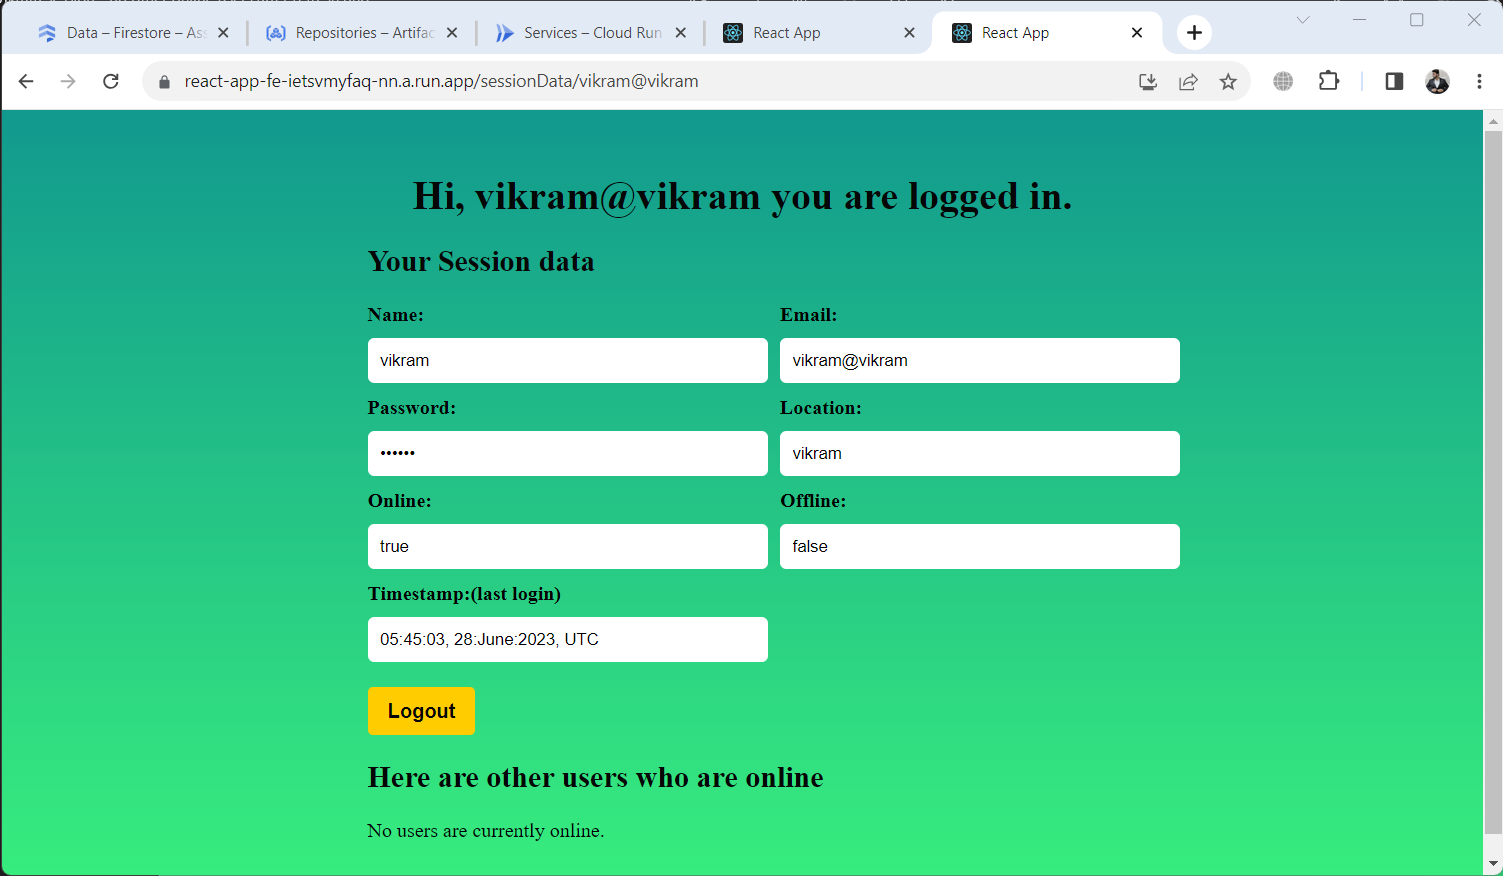
\includegraphics[scale=1, width=15cm,height=7.5cm]{PROBLEM 2/Screenshots/2. Demo/7.1 vikram session - no other online users after refresh.png}}
    \caption{\textbf{\textit{ User - Vikram: no users are online after user: test logged out (after refreshing the page) }}}
    \label{fig:vikram-session-after-test-logout}
\end{figure}

\begin{figure}[htp]
    \centering
    \fbox{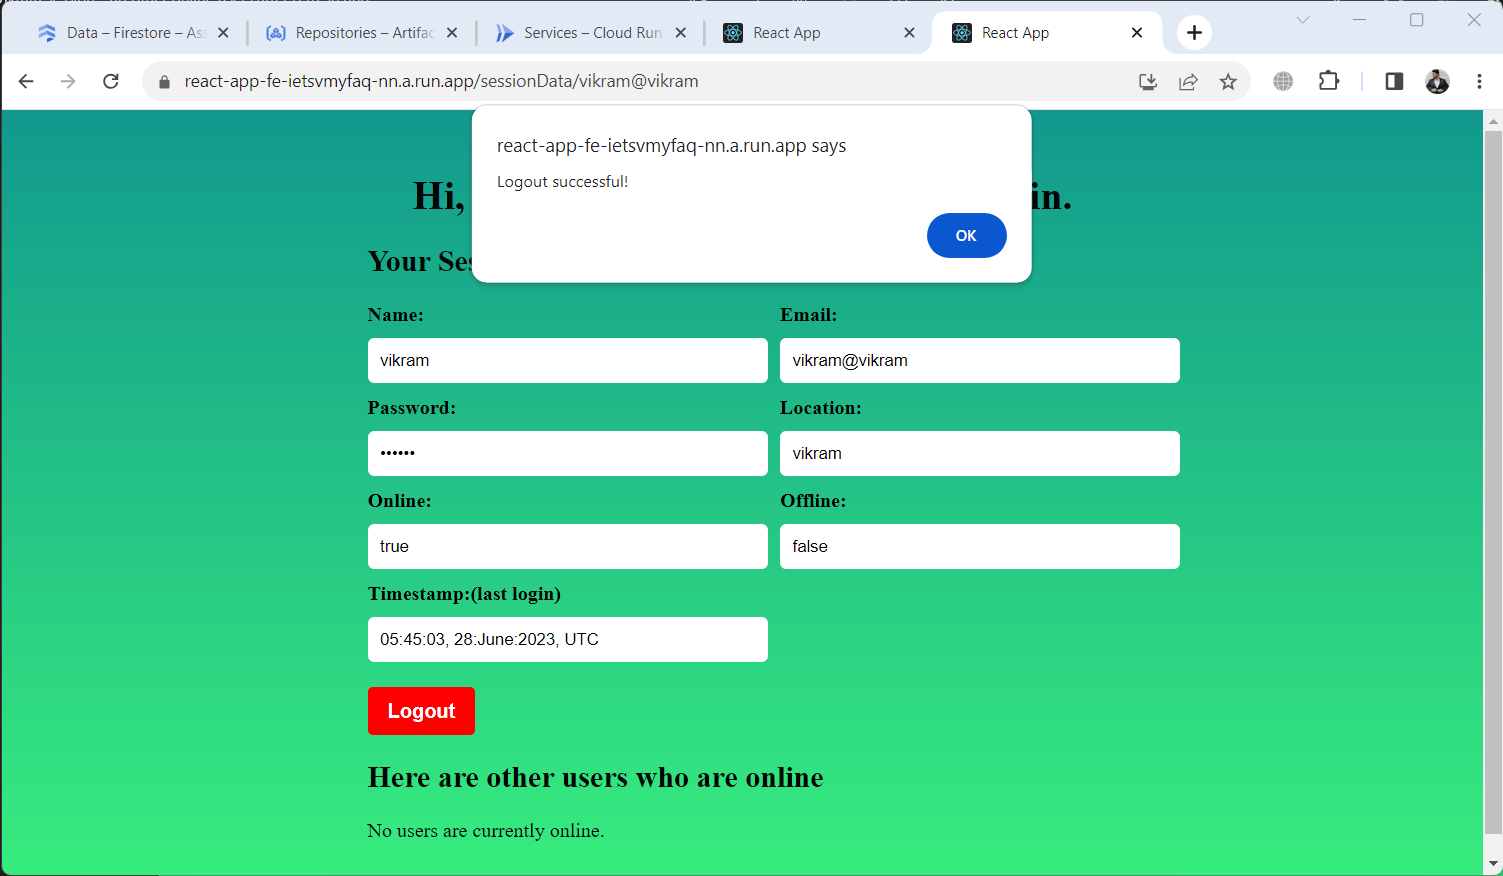
\includegraphics[scale=1, width=15cm,height=7.5cm]{PROBLEM 2/Screenshots/2. Demo/7.2 vikram - logout success.png}}
    \caption{\textbf{\textit{User - Vikram: Logout success}}}
    \label{fig:vikram-logout-success}
\end{figure}

\begin{figure}[htp]
    \centering
    \fbox{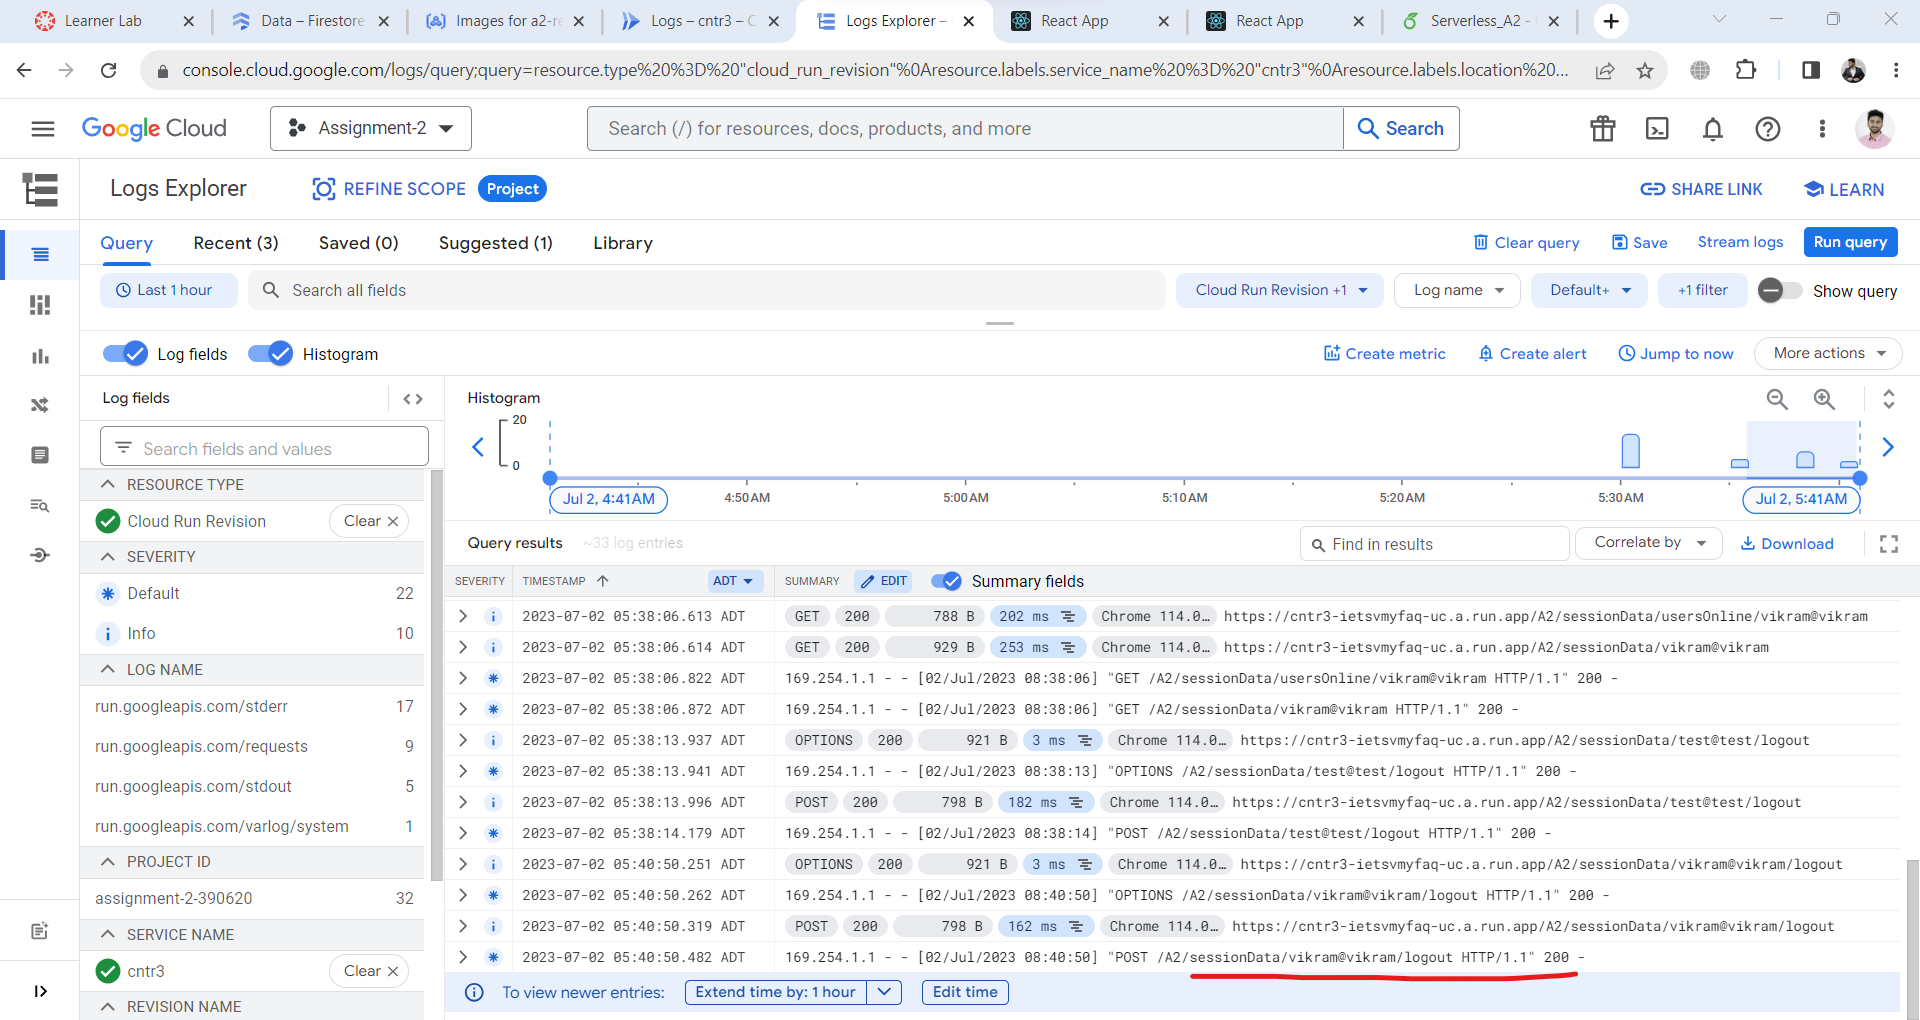
\includegraphics[scale=1, width=15cm,height=7.5cm]{PROBLEM 2/Screenshots/2. Demo/1. Logs/5. vikram session logout.png}}
    \caption{\textbf{\textit{User - Vikram: Logout logs}}}
    \label{fig:vikram-logout-success}
\end{figure}
\begin{figure}[htp]
    \centering
    \fbox{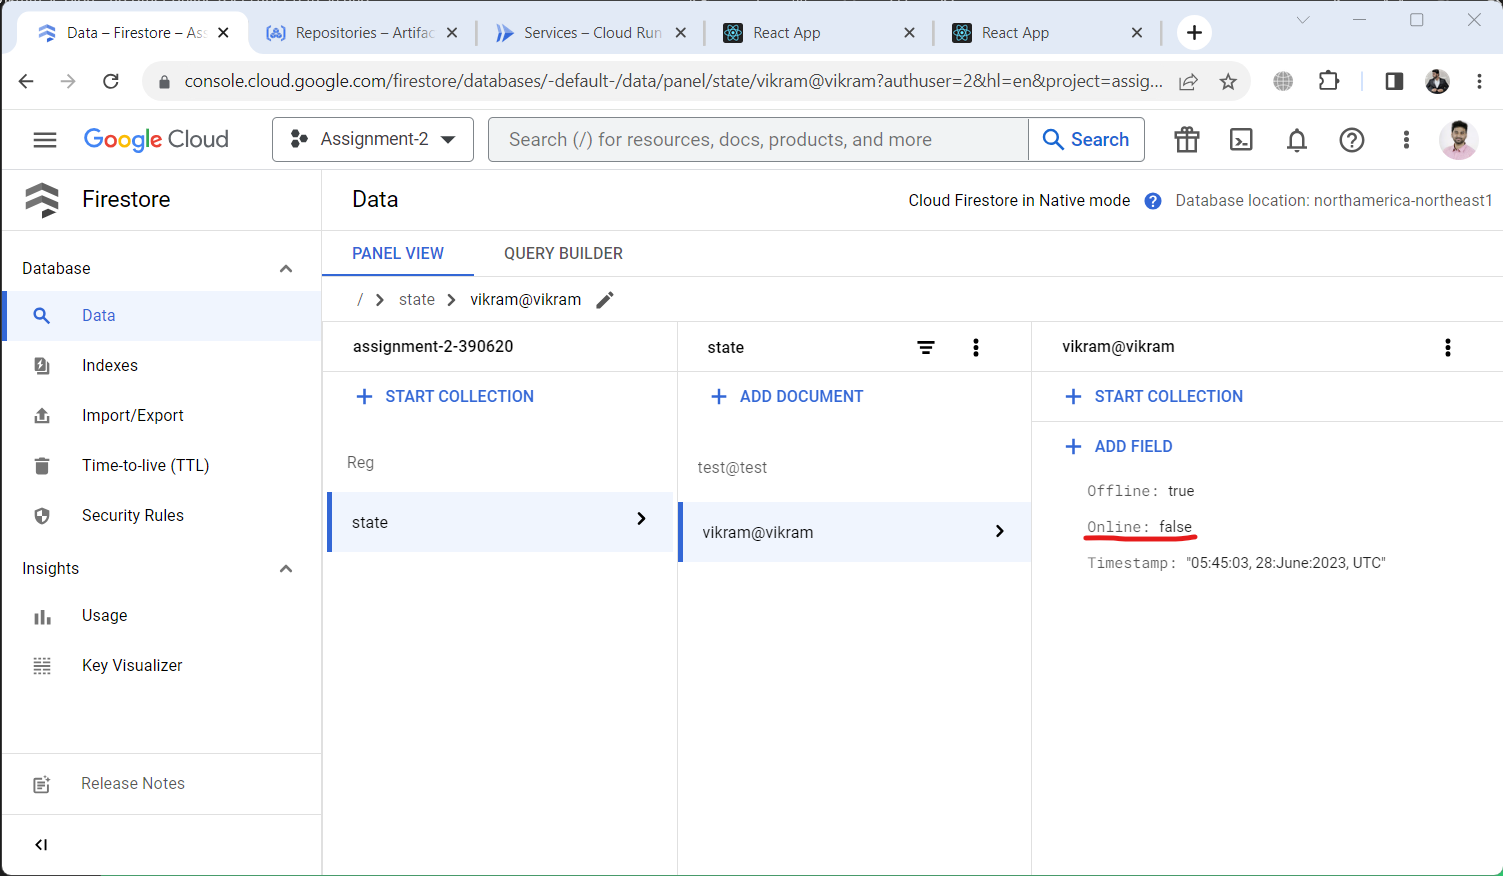
\includegraphics[scale=1, width=15cm,height=7.5cm]{PROBLEM 2/Screenshots/2. Demo/7.3 vikram session - offline after logout.png}}
    \caption{\textbf{\textit{User - Vikram: Session is offline}}}
    \label{fig:vikram-session-offline}
\end{figure}

\newpage\newpage
\section{Test cases}
\begin{figure}[htp]
    \centering
    \fbox{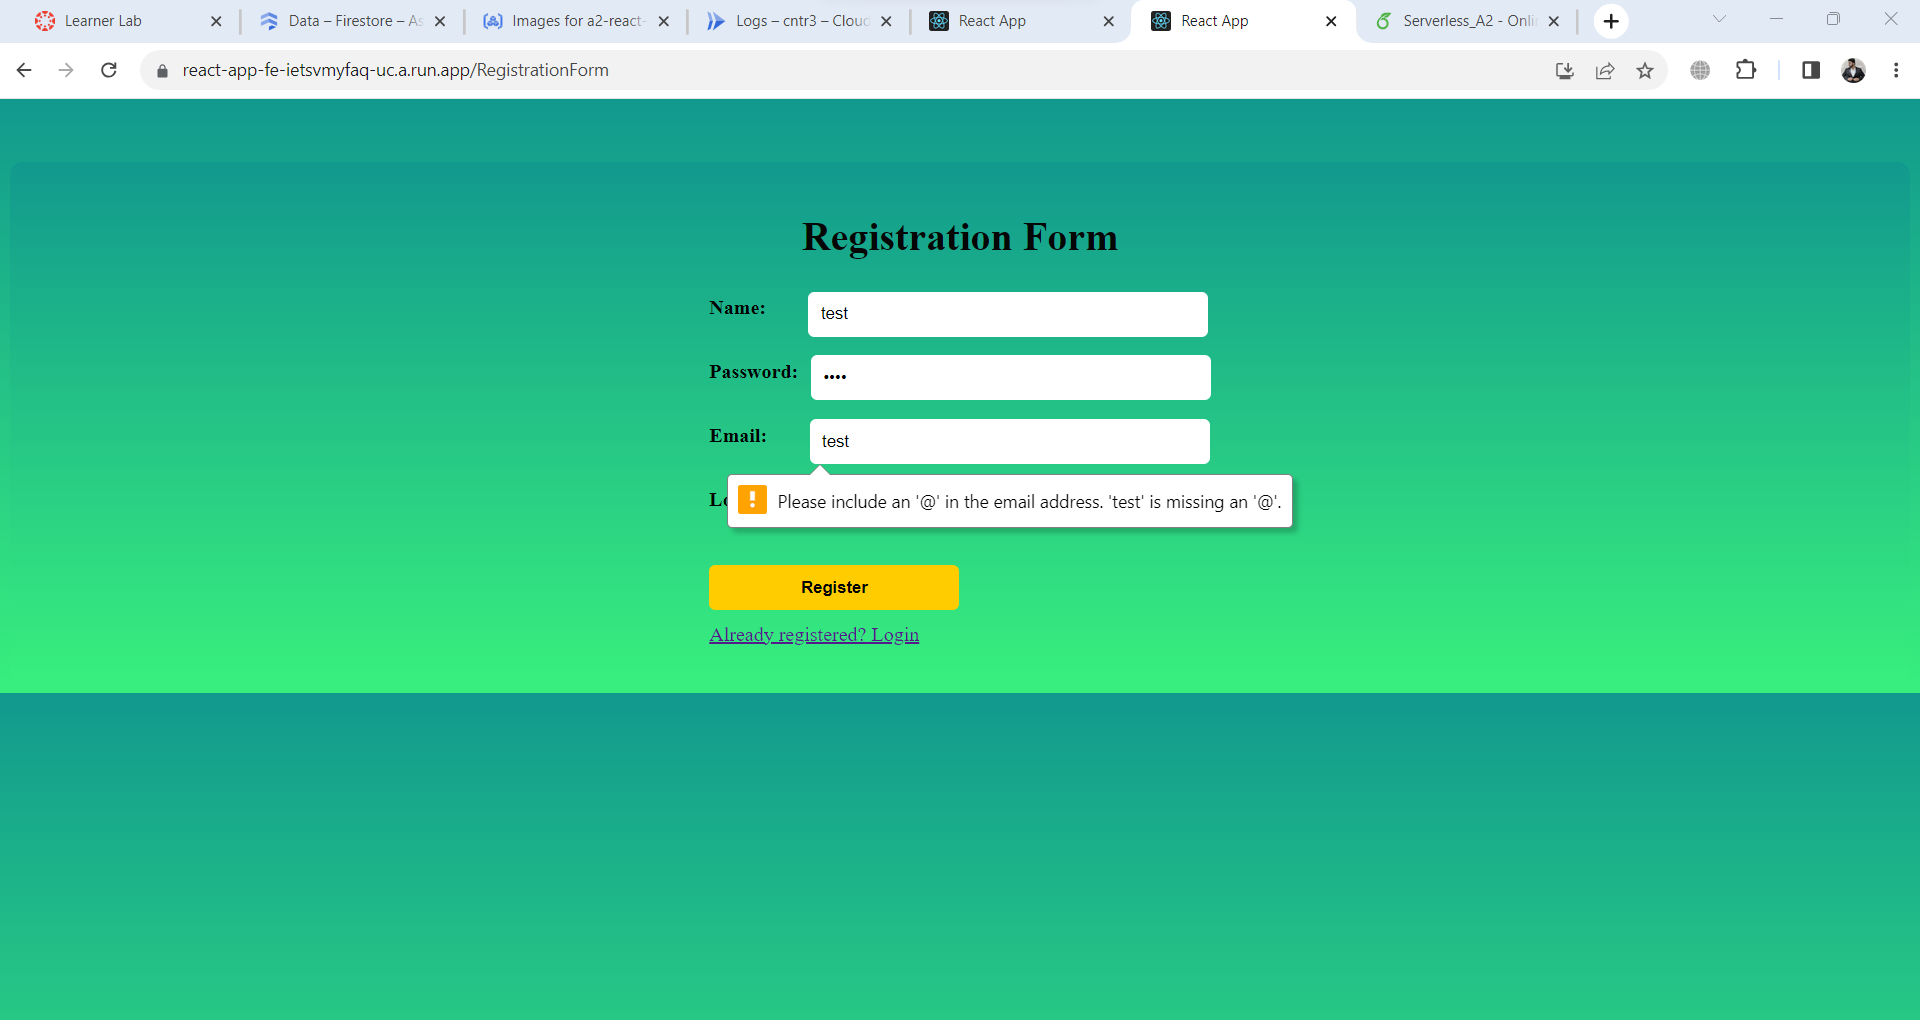
\includegraphics[scale=1, width=15cm,height=7.5cm]{PROBLEM 2/Screenshots/4. Test case/0. email needs @.png}}
    \caption{\textbf{\textit{Email validation - must have '@' symbol}}}
    \label{fig:test-case-invalid-creds}
\end{figure}
\begin{figure}[htp]
    \centering
    \fbox{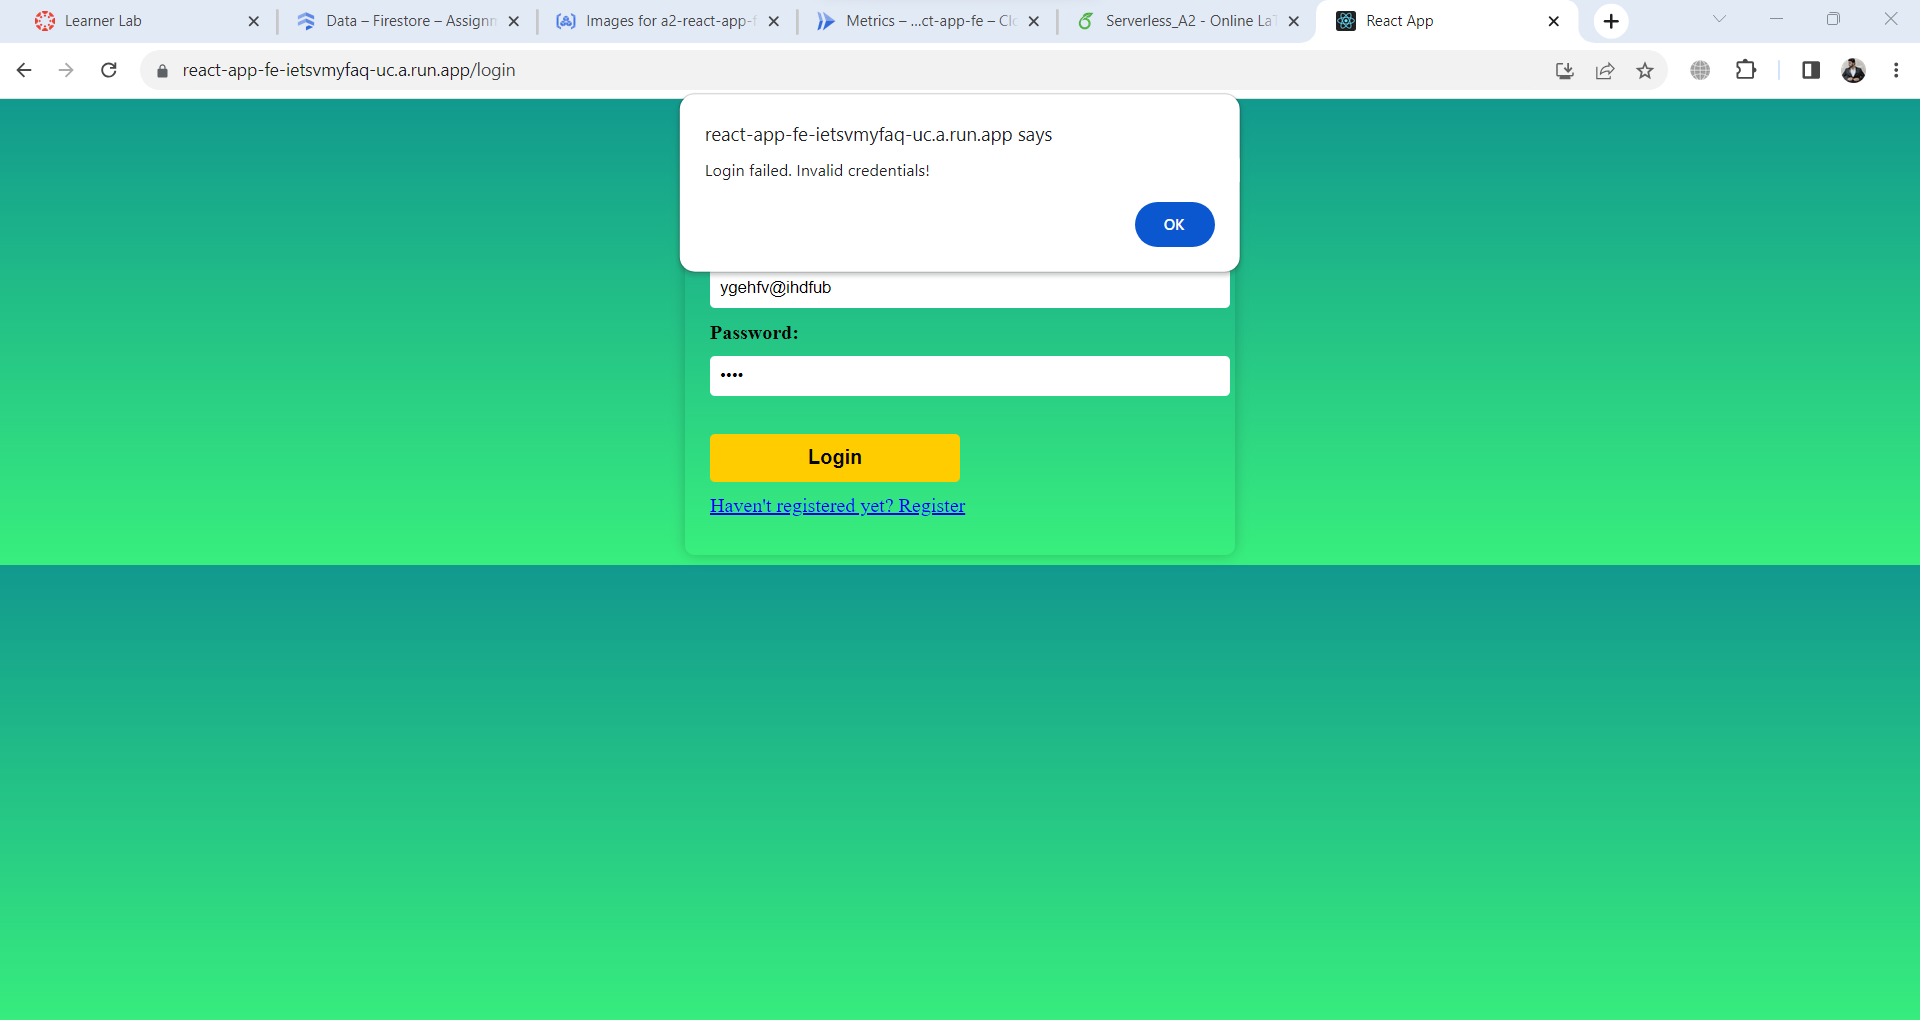
\includegraphics[scale=1, width=15cm,height=7.5cm]{PROBLEM 2/Screenshots/4. Test case/1. invalid credentials.png}}
    \caption{\textbf{\textit{Input: random credentials, Error: "Invalid credentials" - Since the record is not present in the collection "Reg"}}}
    \label{fig:test-case-invalid-creds}
\end{figure}
\begin{figure}[htp]
    \centering
    \fbox{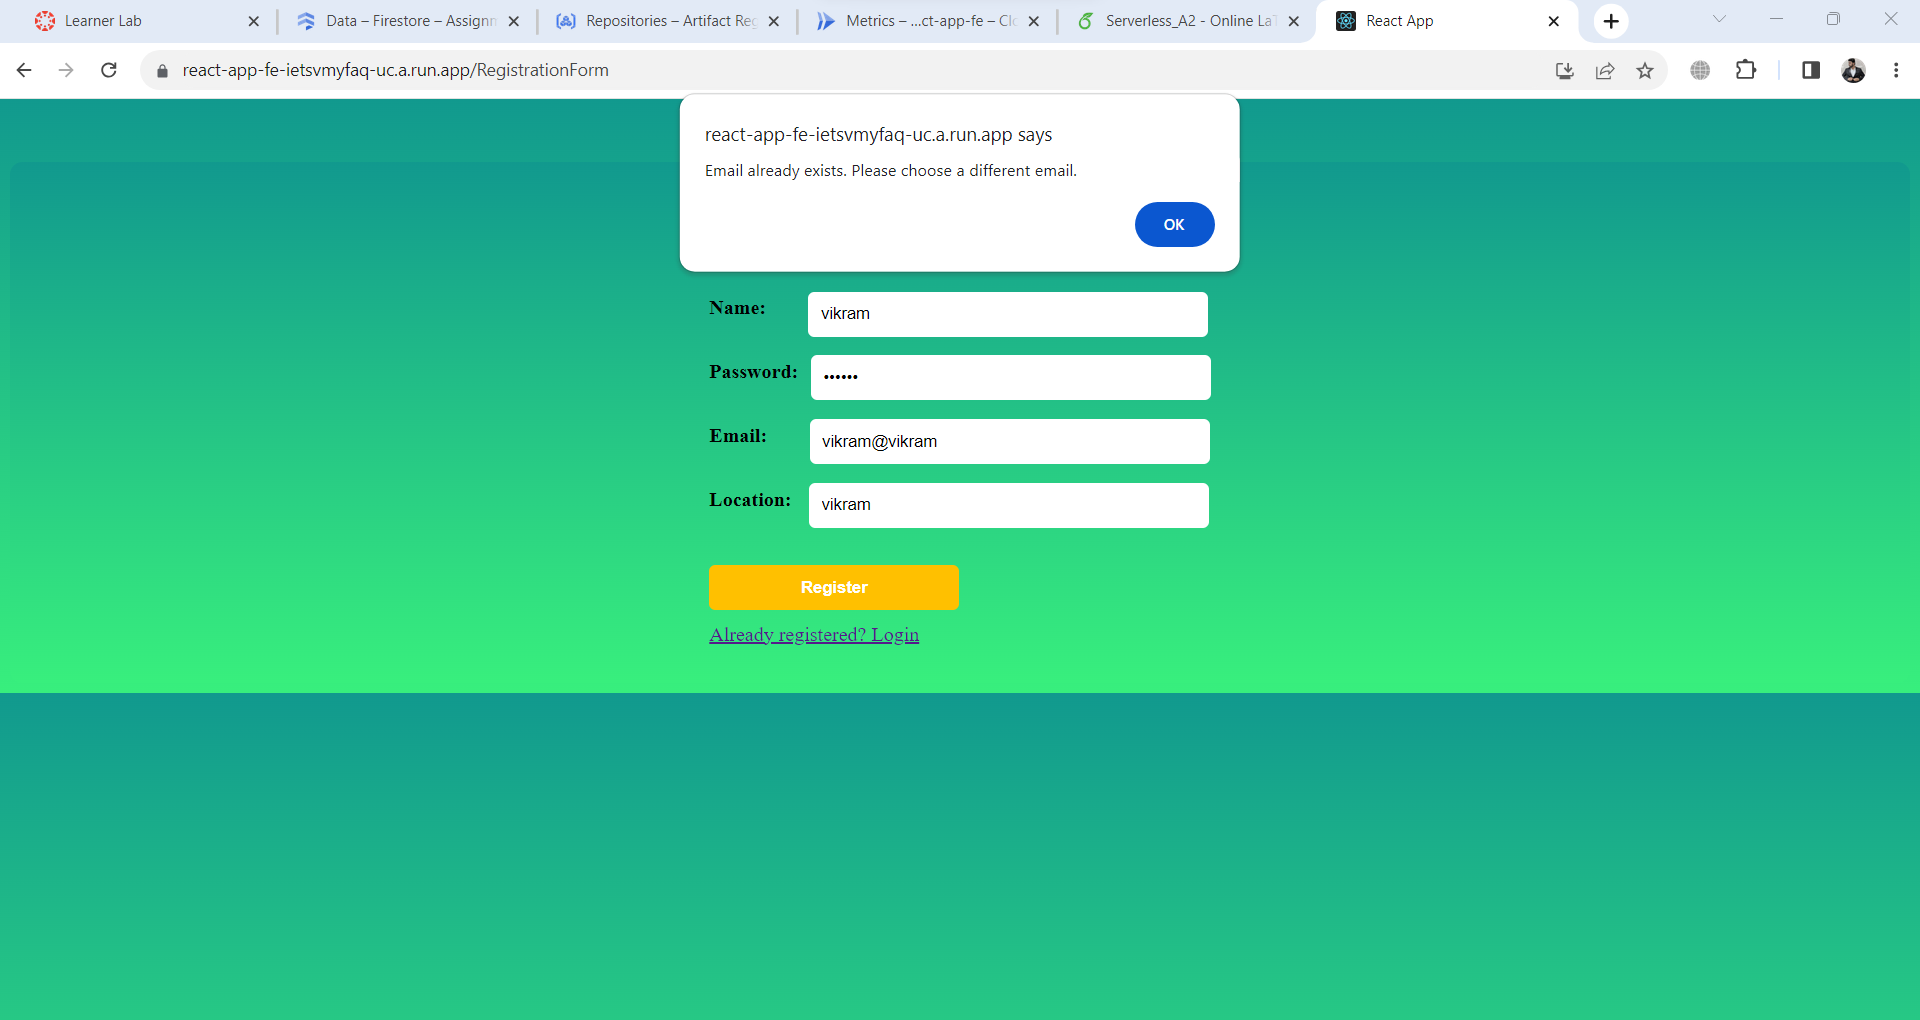
\includegraphics[scale=1, width=15cm,height=7.5cm]{PROBLEM 2/Screenshots/4. Test case/2. email already exists.png}}
    \caption{\textbf{\textit{Input: registration with an already existing email. Error: "Email already exists" - indicating that the entered email is already present in the collection "Reg"}}}
    \label{fig:test-case-email-exists}
\end{figure}

\begin{figure}[htp]
    \centering
    \fbox{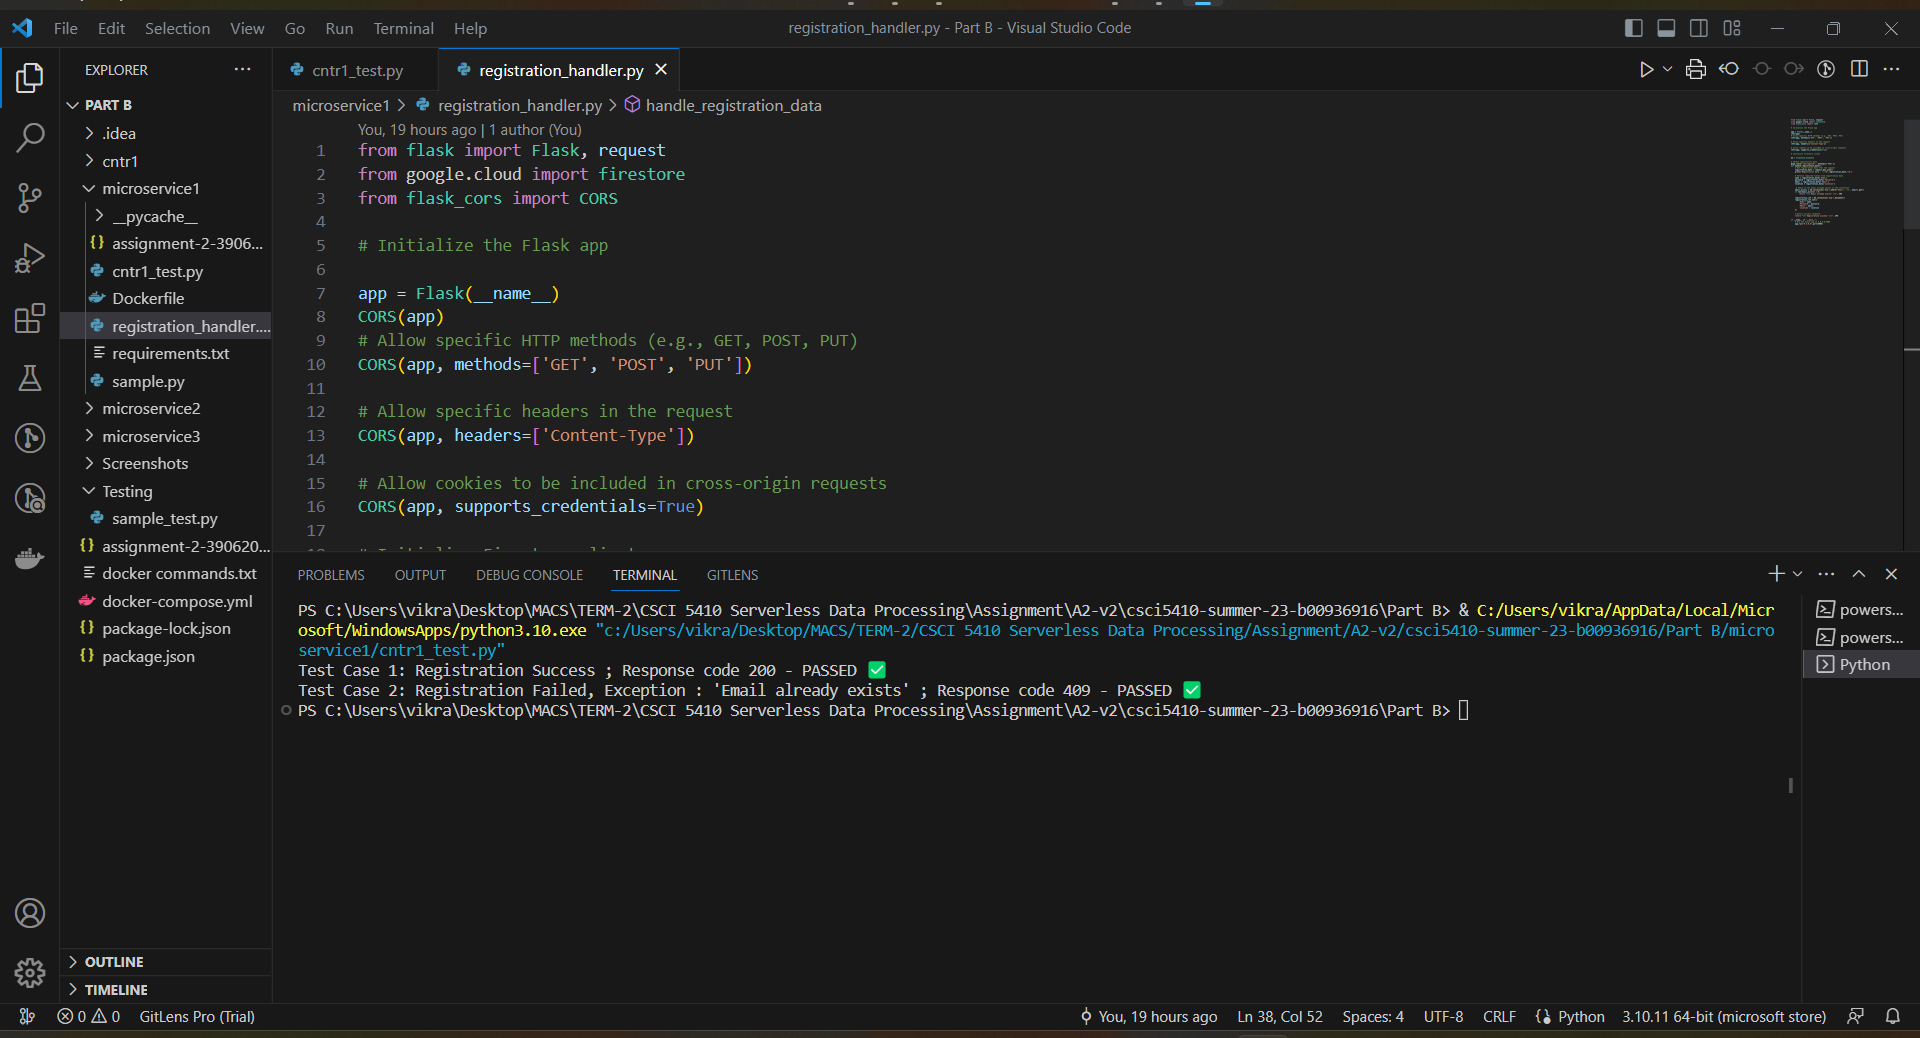
\includegraphics[scale=1, width=15cm,height=7.5cm]{PROBLEM 2/Screenshots/4. Test case/Backend/1. cntr1 test cases passed.png}}
    \caption{\textbf{\textit{Test cases for container 1}}}
    \label{fig:test-case-container-1}
\end{figure}

\begin{figure}[htp]
    \centering
    \fbox{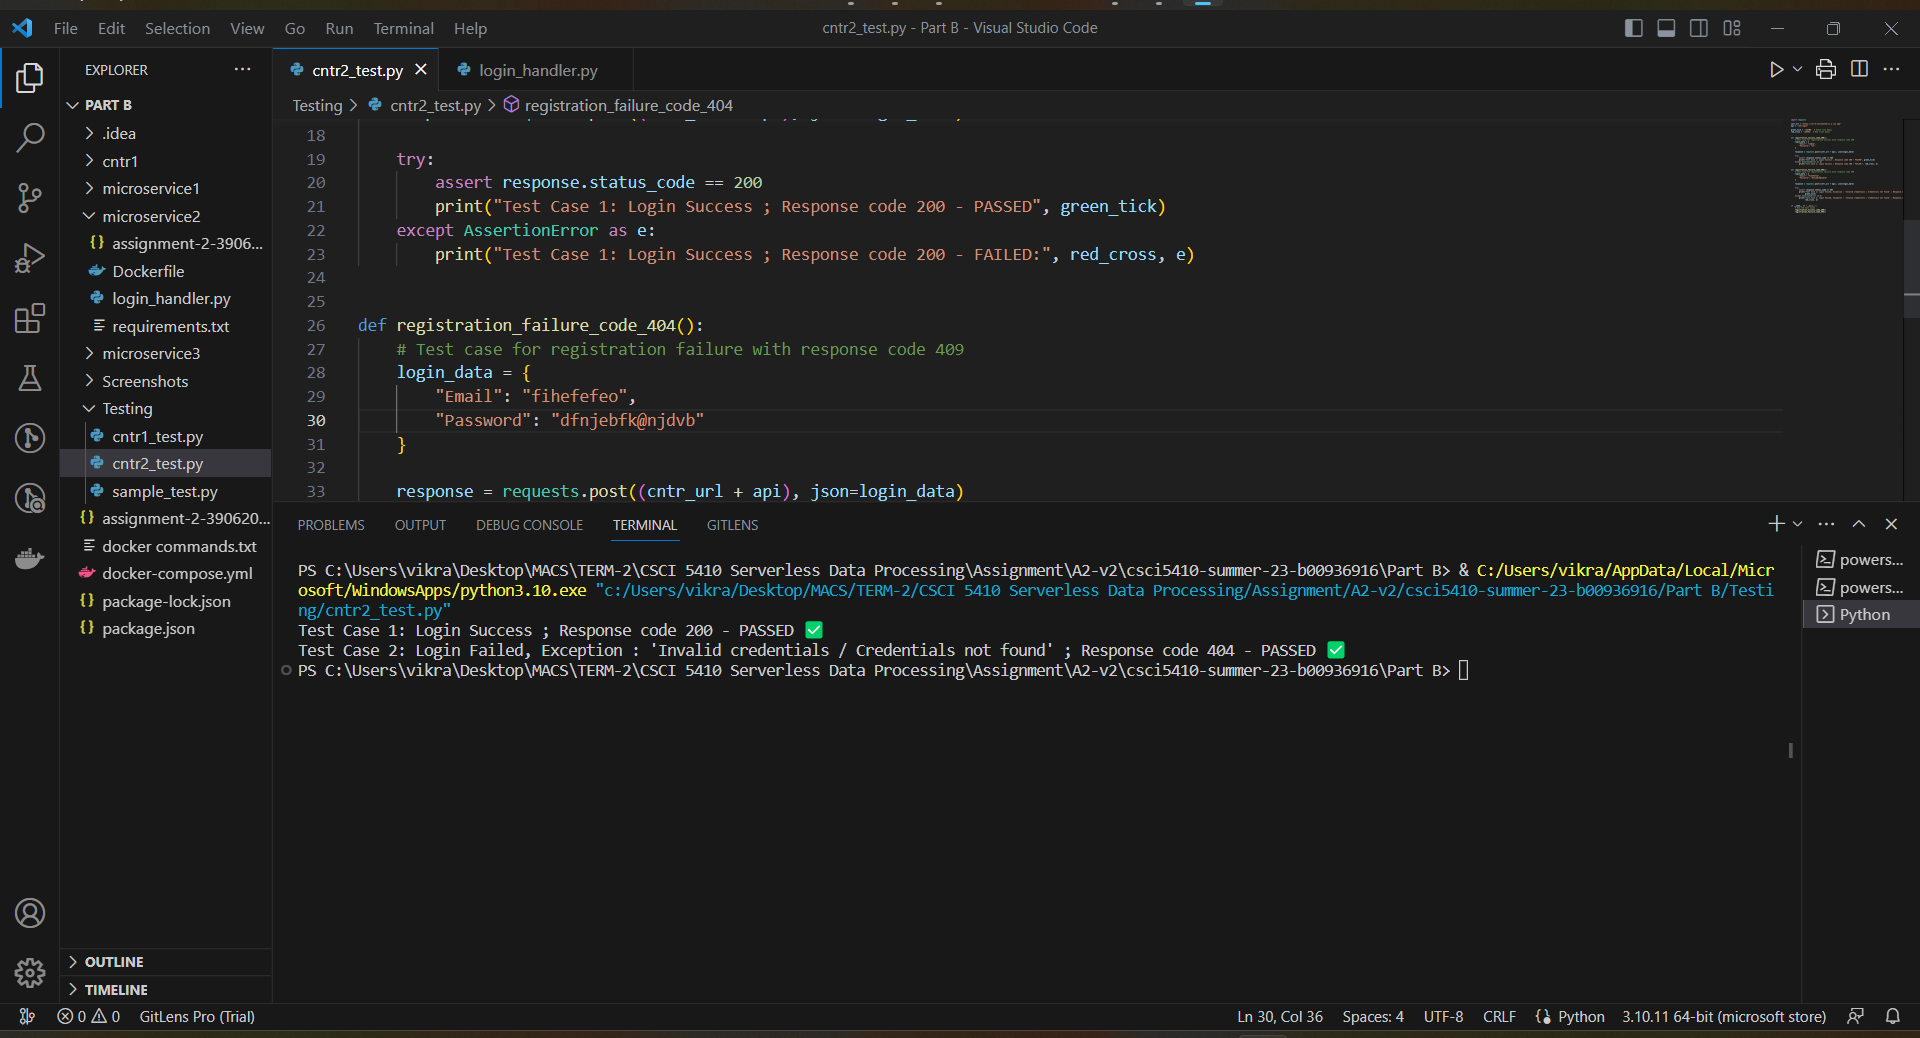
\includegraphics[scale=1, width=15cm,height=7.5cm]{PROBLEM 2/Screenshots/4. Test case/Backend/2. cntr2 test cases passed.png}}
    \caption{\textbf{\textit{Test cases for container 2}}}
    \label{fig:test-case-container-2}
\end{figure}

\begin{figure}[htp]
    \centering
    \fbox{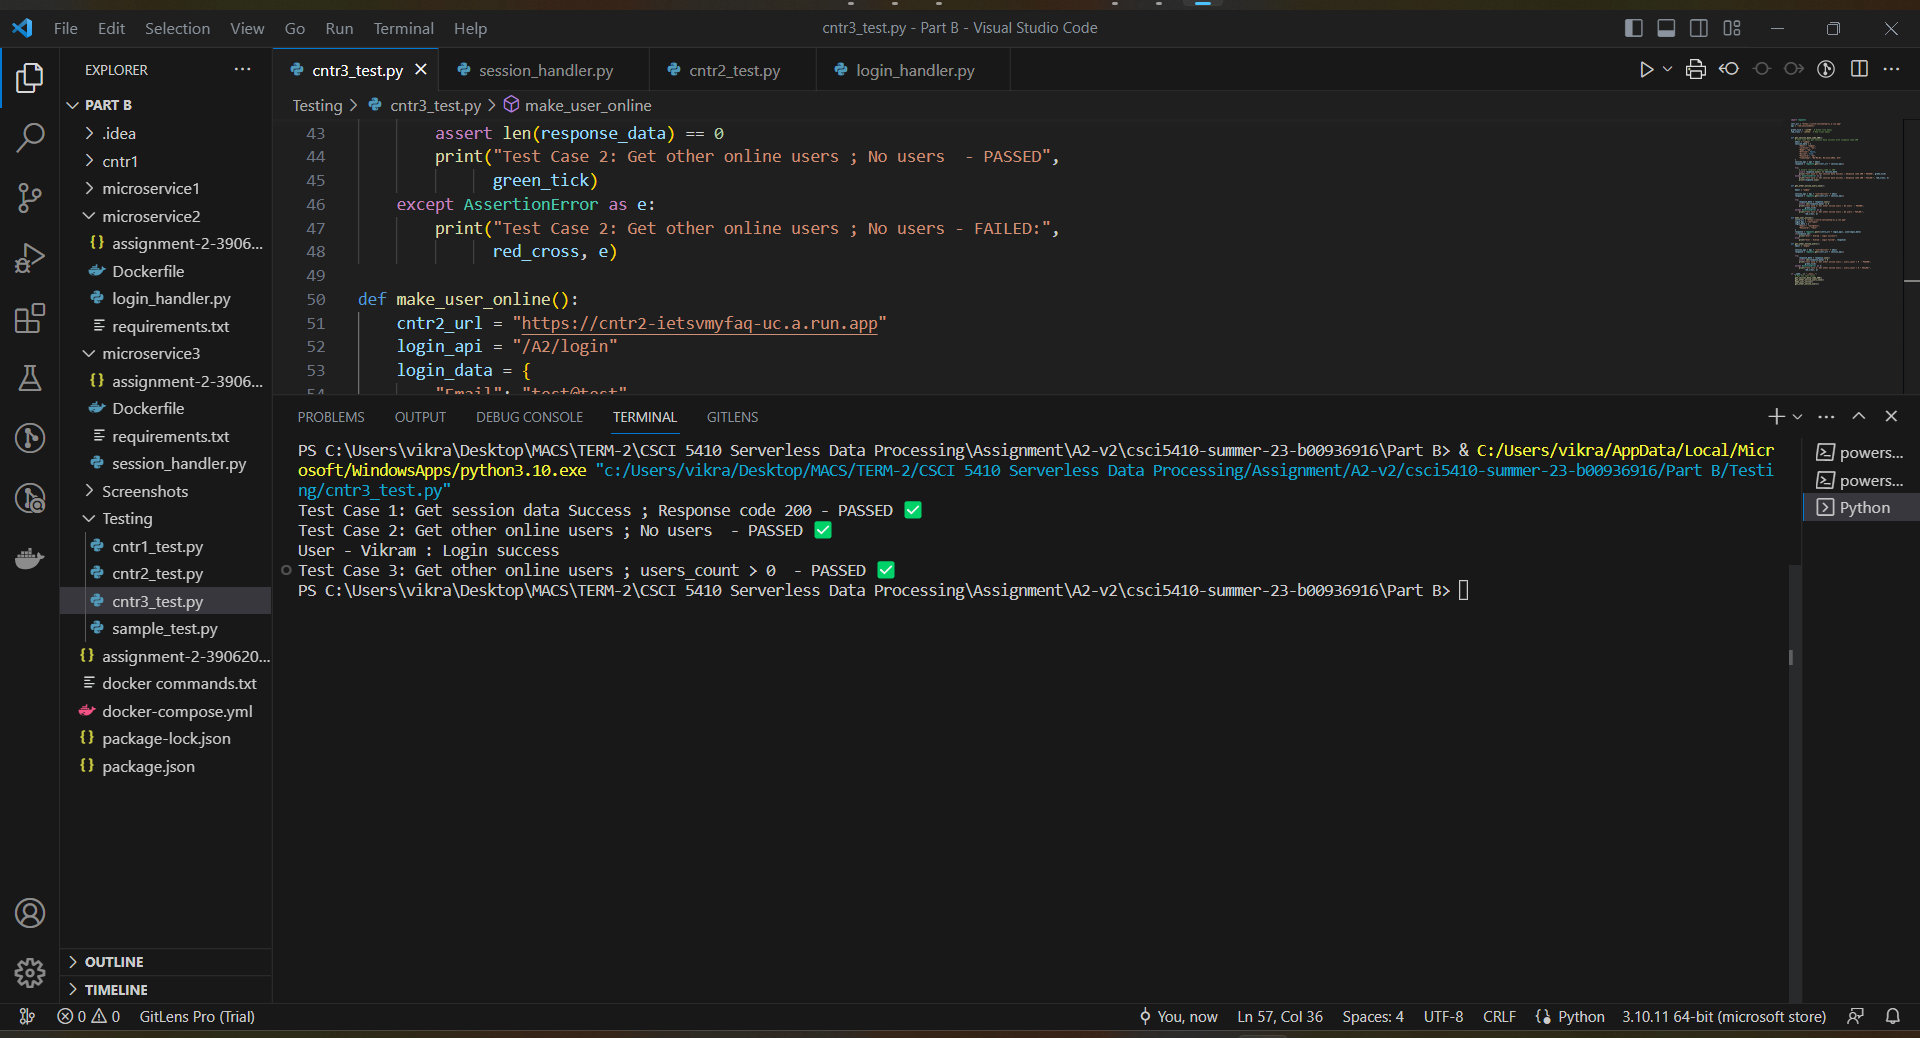
\includegraphics[scale=1, width=15cm,height=7.5cm]{PROBLEM 2/Screenshots/4. Test case/Backend/3. cntr3 session data passed.png}}
    \caption{\textbf{\textit{Test cases for container 3}}}
    \label{fig:test-case-container-3}
\end{figure}

\newpage
\section{My view on leveraging Google Cloud Run, GCR/Artifact Registry, and Docker Containers for Efficient Application Deployment}

My application relies on the power of Google Cloud technologies to achieve seamless deployment and management. By utilizing Google Cloud Run[3], I can deploy my application as stateless containers, benefitting from automatic scaling and secure execution. This allows me to focus on developing my application code while leaving the infrastructure complexities to Cloud Run.
\newline\newline
To store and manage my container images, I utilized Google Artifact Registry[2]. This central repository enabled me to version control my images, control access to containers, and efficiently distribute them across different environments. With easy push and pull capabilities[8], I can ensure smooth deployment and updates[7] of my container images.
\newline\newline
Docker containers[6] play a vital role in the deployment process. They encapsulate the application code, dependencies, and configurations, making deployments consistent and portable. Docker's containerization technology provides isolation, scalability, and optimized resource utilization, contributing to improved performance and maintainability of the application.
\newline\newline
 \textbf{My personal observation:}
 \newline
During the process of pushing Docker images to Artifact Registry, I observed an interesting behavior. When pushing the "cnt2" images, I noticed that instead of uploading all the layers from scratch, the system fetched some layers from the previously pushed "cntr1" images (Refer figures \ref{fig:push-container-1},\ref{fig:push-container-2},\ref{fig:push-container-3}). Since these layers were identical, reusing them saved valuable time and resources. This optimization in the image pushing process demonstrates the efficiency of Google Artifact Registry in handling and managing container images, further enhancing the overall deployment experience.
\newline\newline
In conclusion, my application benefits from Google Cloud Run's scalability, Artifact Registry's image management capabilities, and Docker containers' consistency and portability. These technologies work harmoniously to provide me with an efficient, secure, and easily manageable application infrastructure. Additionally, Docker and Google Cloud Platform offer extensive documentation and resources, which enabled me to maximize the benefits of these tools in my application development and deployment process.









% \begin{figure}[htp]
%     \centering
%     \fbox{\includegraphics[scale=1, width=15cm,height=7.5cm]{PROBLEM 2/}
%     \caption{\textbf{\textit{ }}}}
%     \label{fig:}
% \end{figure}


\newpage